\documentclass[numbers=noenddot, 12pt, listof=totoc, bibliography=totoc]{scrbook}

\usepackage[utf8]{inputenc}
\usepackage[T1]{fontenc}

\usepackage[maxbibnames=99,maxcitenames=2,uniquelist=false,backend=biber,terseinits=true,bibstyle=authoryear,giveninits=true,uniquename=init,citestyle=authoryear]{biblatex}
\urlstyle{same}
\DeclareNameAlias{sortname}{family-given}
\addbibresource{Thesis/0008_Literature.bib}

\usepackage{csquotes}
\usepackage[english]{babel}

\usepackage[onehalfspacing]{setspace}
\usepackage[twoside,bindingoffset=2cm,right=2cm,top=3cm,bottom=3cm,left=2cm,a4paper]{geometry}

\usepackage[automark,headsepline,plainheadsepline]{scrlayer-scrpage}
\automark[section]{chapter}

\usepackage{ragged2e}

\usepackage{blindtext}

\usepackage[pdfpagelabels]{hyperref}

\usepackage{graphicx}
\usepackage{varwidth}

\usepackage{bm}

\usepackage{rotating}

\usepackage{newtxtext}
%\usepackage[slantedGreek]{newtxmath}
\usepackage{newtxmath}

\usepackage[acronyms, toc, automake=false, counter=chapter,  nopostdot, nonumberlist]{glossaries}
\makenoidxglossaries

\usepackage{calc}

\usepackage{pdfpages}

\usepackage{pgfplots}
\usepackage{pgfplotstable}
\pgfplotsset{compat=newest}

\usepackage{booktabs}
%\usepackage{tabularx}
\usepackage{multirow}
\usepackage{longtable}
\usepackage{colortbl}
\usepackage{array}

\usepackage{textgreek}
\usepackage{wasysym}
\usepackage{amsmath}
\usepackage{empheq}
\usepackage{amsfonts}

\usepackage{enumitem}

%\usepackage{extarrows}
\usepackage{chngcntr}

\usepackage{float}
%\usepackage{floatrow}
\usepackage[labelfont=bf, font=footnotesize, labelsep=space, format=plain, labelformat = simple, nooneline, aboveskip=10pt, belowskip=10pt]{caption}
\usepackage[labelfont=bf, font=footnotesize, labelsep=space, format=plain, list=false, labelformat=parens, aboveskip=0pt, belowskip=0pt, justification=centering, listformat=simple]{subcaption}

%listformat option macht zahlen dazu
%\floatsetup[longtable]{LTcapwidth=table}

\usepackage{newfloat}
\DeclareFloatingEnvironment[
    fileext=lop,
    name=Gl.,
    within=section,
]{fequation}

\usepackage[export]{adjustbox}

\usepackage{fancyvrb}

\usepackage{tikz}
\usetikzlibrary{fadings,shapes.arrows,shadows}   

\usepackage{framed}
\usepackage{listings}
\usepackage{xcolor}

\definecolor{codegreen}{rgb}{0,0.6,0}
\definecolor{codegray}{rgb}{0.5,0.5,0.5}
\definecolor{codepurple}{rgb}{0.58,0,0.82}
\definecolor{backcolour}{rgb}{0.95,0.95,0.92}

\lstdefinestyle{mystyle}{
    backgroundcolor=\color{backcolour},   
    commentstyle=\color{codegreen},
    keywordstyle=\color{magenta},
    numberstyle=\tiny\color{codegray},
    stringstyle=\color{codepurple},
    basicstyle=\ttfamily\footnotesize,
    breakatwhitespace=false,         
    breaklines=true,                 
    captionpos=b,                    
    keepspaces=true,                 
    numbers=left,                    
    numbersep=5pt,                  
    showspaces=false,                
    showstringspaces=false,
    showtabs=false,                  
    tabsize=2
}

\lstset{style=mystyle}

\DefineBibliographyStrings{english}{andothers={et\ al\adddot}}

\usepackage[section]{placeins}
%float only inside its section
%\FloatBarrier extra command

\newacronym{UMAP}{UMAP}{Uniform Manifold Approximation and Projection}
\newacronym{PCA}{PCA}{Principal Component Analysis}
\newacronym{HDBSCAN}{HDBSCAN}{Hierarchical Density-Based Spatial Clustering of Applications with Noise}
\newacronym{IAV}{IAV}{\textit{Influenza A Virus}}
\newacronym{HA}{HA}{hemagglutinin}
\newacronym{NA}{NA}{neuraminidase}
\newacronym{M1}{M1}{matrix protein 1}
\newacronym{PB1}{PB1}{polimerase basic protein 1}
\newacronym{PB2}{PB2}{polimerase basic protein 2}
\newacronym{PA}{PA}{polimerase acid protein}
\newacronym{NS1}{NS1}{nonstructural protein 1}
\newacronym{NP}{NP}{viral ribonucleoprotein}
\newacronym{NEP}{NEP}{nuclear export protein}
\newacronym{HEF}{HEF}{hemagluthinin-esterase-fusion}
\newacronym{M2}{M2}{M2 ion channel}
\newacronym{BM2}{BM2}{BM2 ion channel}
\newacronym{CM2}{CM2}{CM2 ion channel}
\newacronym{NB}{NB}{NB ion channel}
\newacronym{MSA}{MSA}{Multiple Sequence Alignment}
\newacronym{DBCV}{DBCV}{Density Based Cluster Validity}
\newacronym{UPGMA}{UPGMA}{Unweighted Pair Group Method with Arithmetic mean}
\newacronym{API}{API}{Application Programming Interface}
%\newacronym[shortplural=SNPs, longplural=single nucleotide polymorphisms]{SNP}{SNP}{single nucleotide polymorphism}
%\newacronym[shortplural=AAs, longplural=aminoacids]{AA}{AA}{aminoacids}

\begin{document}
    
    \selectlanguage{english}

\setkomafont{disposition}{\normalfont\bfseries}

\raggedbottom

\allowdisplaybreaks[1]

\renewcommand*{\headfont}{\normalfont}

\clearpairofpagestyles
\lehead*{\pagemark}
\rohead*{\pagemark}
\lohead{\rightmark}
\rehead{\leftmark}

\renewcommand{\figurename}{Fig.}
\renewcommand{\figureautorefname}{Fig.}
\renewcommand{\tablename}{Tab.}
\renewcommand{\tableautorefname}{Tab.}
\renewcommand{\chapterautorefname}{Chap.}
\renewcommand{\sectionautorefname}{Sec.}
\renewcommand{\subsectionautorefname}{Subsec.}
\renewcommand{\subsubsectionautorefname}{Subsubsec.}
%\renewcommand{\lstlistingname}{Lst.}

\renewcommand{\thetable}{\thechapter.\arabic{table}}
\renewcommand{\thefigure}{\thechapter.\arabic{figure}}
\renewcommand{\theequation}{\thechapter.\arabic{equation}}
\renewcommand{\thelstlisting}{\thechapter.\arabic{lstlisting}}

\renewcommand{\thesubtable}{\Alph{subtable}}
\renewcommand{\thesubfigure}{\Alph{subfigure}}

\renewcommand*{\chaptermarkformat}{}
\renewcommand*{\sectionmarkformat}{}
\renewcommand*{\subsectionmarkformat}{}

\newcolumntype{L}{>{\raggedright\arraybackslash}X}
\newcolumntype{C}{>{\centering\arraybackslash}X}
\newcolumntype{R}{>{\raggedleft\arraybackslash}X}

\newcommand{\ltab}{\raggedright\arraybackslash}
\newcommand{\ctab}{\centering\arraybackslash}
\newcommand{\rtab}{\raggedleft\arraybackslash}

\newenvironment{nstabbing}
    {\setlength{\topsep}{0pt}%
    \setlength{\partopsep}{0pt}%
    \tabbing}
    {\endtabbing}
    
\newenvironment{nsitemize}
    {\setlength{\topsep}{0pt}%
    \setlength{\partopsep}{0pt}%
    \itemize}
    {\enditemize}

\setlength\parindent{0pt}
\setlength{\parskip}{0pt}

\pgfplotstableset{
    empty cells with={---},
    font=\footnotesize,
    precision=3,
    col sep=comma,
}
    %\makeatletter
\renewcommand\frontmatter{%
    \cleardoublepage
    \@mainmatterfalse
    %\pagenumbering{gobble}
    %\pagenumbering{roman}
}

\renewcommand\mainmatter{%
    \cleardoublepage
    \@mainmattertrue
    \pagenumbering{arabic}
    \setcounter{page}{7}
}

\renewcommand\backmatter{%
    \if@openright
        \cleardoublepage
    \else
        \clearpage
    \fi
    \@mainmatterfalse
    %\pagenumbering{gobble}
}
\makeatother
    
    \frontmatter
    \pagestyle{empty} 
    \renewcommand*{\chapterpagestyle}{empty}

    \begin{titlepage}
    
    \centering 
    \large
    
\includegraphics[width=0.5\textwidth]{Graphics/Logo.jpg}

    \vspace{5em}

    {\Large \textbf{Large Scale Reevaluation of \textit{Influenza A Virus} Classification based on $\bm{k}$-mer frequencies}}
    
    \vspace{5em}
    
    M~A~S~T~E~R~A~R~B~E~I~T
    
    \vspace{1em}
    
    zur Erlangung des akademischen Grades
    
    \vspace{1em}
    
    Master of Science (M. Sc.)
    
    im Studiengang Bioinformatik
    
    \vspace{1em}
    
    FRIEDRICH-SCHILLER-UNIVERSITÄT JENA
    
    Fakultät für Mathematik und Informatik
    
    \vfill
    
    eingereicht von Alexander Henoch
    
    geb. am 02.02.1995 in Bremen
    
    \vspace{1em}
    
    Betreuer: Prof. Dr. Manja Marz
    
    \vspace{1em}
    
    Jena, den 14.07.2021
    
\end{titlepage}
    
    \chapter*{Zusammenfassung}

    \blindtext
    
    \chapter*{Abstract}

Reoccurring local outbreaks of new, highly pathogenic strains of the \gls{IAV}, picture a unnoticed but still persisting major danger to the whole human population, that reached global extend with high numbers of fatalities, several times in the past. Due to the lack of a cure, resort to vaccines producing varying levels of immunization with yearly expiration is inevitable. For better preparation on possible future pandemics, enlarging the knowledge of the \gls{IAV} is crucial. High evolution-rates by more drastic mutation mechanisms of the \gls{IAV} and a classification giving little insight, complicate accurate novel research though. This thesis, serves the elaboration of a segment-wise clustering pipeline, usable on all sequenced genomes of \gls{IAV}. Instead of being alignment based, this method utilizes the better scalablity of $k$-mer frequency vectors, with the novel hybrid clustering implementation of \texttt{HDBSCAN}, connecting hierarchical with density-based clustering. Appropriate parameters were selected by different validation techniques and well-known tools were used for dimension reduction of the vectors. By in depth comparison of the results, a workflow combining a novel vector clustering method with validated parameters, posterior to an efficient dimension reduction, is proposed. 
    
    \mainmatter
    \pagestyle{scrheadings} 
    \renewcommand*{\chapterpagestyle}{plain}
    \KOMAoptions{cleardoublepage=headings}
    
    \tableofcontents
    
    \glsaddall 
    \setglossarystyle{listgroup}
    \printnoidxglossary[title=List of Abbreviations, type=\acronymtype]
    %\lstlistoflistings

    \chapter{Introduction} \label{chap:Introduction}

\section{Zoonoses and the risks of pandemics}

In times where infectious disease outbreaks become more frequent and sometimes even reach global appearance, unpredictable effects on humans, wildlife and whole ecosystems are inevitable \autocite{schmeller_biodiversity_2020}. Growing human population and persisting poverty has harmful impact on the biodiversity and results in degradation of natural habitats and more frequent human-wildlife contacts  \autocite{schmeller_biodiversity_2020}. Therefore, increasing numbers of zoonoses, transfers of animal pathogens on humans, arise and are a major driving force in pathogen emergence on humans in recent decades \autocite{jones_global_2008}. Most of the human pathogens emerging lately are of animal origin, indeed, up to 75\% \autocite{woolhouse_risk_2001}. Well-known examples of zoonoses are avian and swine flu \gls{HIV}, ebola, \gls{MERS} and \gls{SARS} including the current circulating COVID-19 \autocite{van_reeth_avian_2007, sharp_origins_2011, suwantarat_risks_2015, verity_estimates_2020}.

\vspace{1em}

While zoonoses can be of viral, bacterial and parasitic nature, emergences of higher magnitude, like the mentioned well-known examples, are often linked back to viral infections \autocite{woolhouse_risk_2001}. Harmfulness of viral infections can be diverse, ranging from mostly no sign of infection in the natural hosts to very severe symptoms or death in accidental ones \autocite{wahlgren_influenza_2011}. In contrast to natural hosts, humans, accidental hosts to, e.~g.~, the West Nile Virus, develop disease patterns upon infection and, thereby, are not able to fully support the virus life cycle \autocite{gea-banacloche_west_2004}. High variety in host circulation and transmission ways from such natural or intermediate onto humans as accidental hosts, with long infectious periods without symptoms and high transmission pace have a high risk of pandemic events \autocite{jamison_chapter_2017}. A prominent virus detected in a variety of hosts and known for reoccurring local and global outbreaks in the past is \gls{IAV}, member of the \textit{Orthomyxoviridae} family and also commonly known as flu \autocite{wahlgren_influenza_2011}. Analysis indicate a 1\% chance of a pandemic with millions of deaths every year and is, therefore, the pathogen most likely to be responsible for a sudden severe pandemic \autocite{jamison_chapter_2017}. 

\section{Life-cycle and structure of the \textit{Influenza A Virus}}

In humans, infection by \gls{IAV} affects the upper respiratory tract \autocite{julkunen_inflammatory_2000}. General symptoms like fever, cough and headache characterize the infection \autocite{julkunen_inflammatory_2000}. In some cases complications can occur, resulting in primary viral pneumonia or secondary bacterial pneumonia by bacterial infection \autocite{julkunen_inflammatory_2000}. The virus particles of \gls{IAV}, called virions, are spherical in shape, 80–120nm in size and enveloped by the hosts cell membrane lipids \autocite{oxford_chapter_1987, mudhakir_learning_2009, cann_chapter_2016}. These virions can sustain extensive forces in the hosts body and even survive deformation to around 33\% of the its total diameter \autocite{schaap_effect_2012}. Epithelial cells in the tissue of the respiratory tract, are the main infection area of the virions \autocite{oxford_chapter_1987}. The \gls{IAV} virions attach themselves to the host cells with their surface glycoproteins, the tetrameric \gls{NA} and the trimeric \gls{HA} and enter the cells by clathrin-mediated endocytosis (\autoref{fig:Cycle}) \autocite{wilson_structure_1981, varghese_structure_1983, jones_global_2008, mudhakir_learning_2009}. Equilibration of pH in the process of endocytosis involve the transmembrane protein \gls{M2} of \gls{IAV} \autocite{pielak_influenza_2011}. The surface glycoprotein tails are also connected to the second layer in the \gls{IAV} virions, the \gls{M1} \autocite{ali_influenza_2000}. Following the endocytosis the \gls{RNP} complexes are carried to the hosts cells nucleus by \gls{NPC} for virus replication \autocite{eisfeld_at_2015}. These \gls{RNP} complexes contain the viral \gls{ssRNA}, holding the genetic information, bound to multiple \glspl{NP} and the polymerase complex \autocite{eisfeld_at_2015}. The trimeric polymerase complex including the \gls{PB1}, \gls{PB2} and \gls{PA} is essential for viral replication in the hosts nucleus \autocite{area_3d_2004, eisfeld_at_2015}. \gls{IAV} is a segmented virus, one virion of \gls{IAV} contains eight different short \glspl{ssRNA}, called segments, encoding in total 14 viral proteins \autocite{eisfeld_at_2015}. In the nucleus the eight \glspl{ssRNA} are replicated and transcribed to \glspl{mRNA} with the latter translated to the virions proteins in the cytoplasm \autocite{eisfeld_at_2015}. The translated \gls{NEP}, \gls{M1}, \gls{NP} and proteins of the polymerase complex are imported by the \gls{NPC} to build new \glspl{RNP} with the replicated genomes and enable the nuclear exit \autocite{eisfeld_at_2015}. By budding through the plasma membrane with the translated \gls{M2} and \gls{NA}, while incorporating these proteins including \gls{HA} into the surface, new virions are released coated in the host cell membrane lipids \autocite{eisfeld_at_2015}.

\begin{figure}[!hbt]
    \centering
    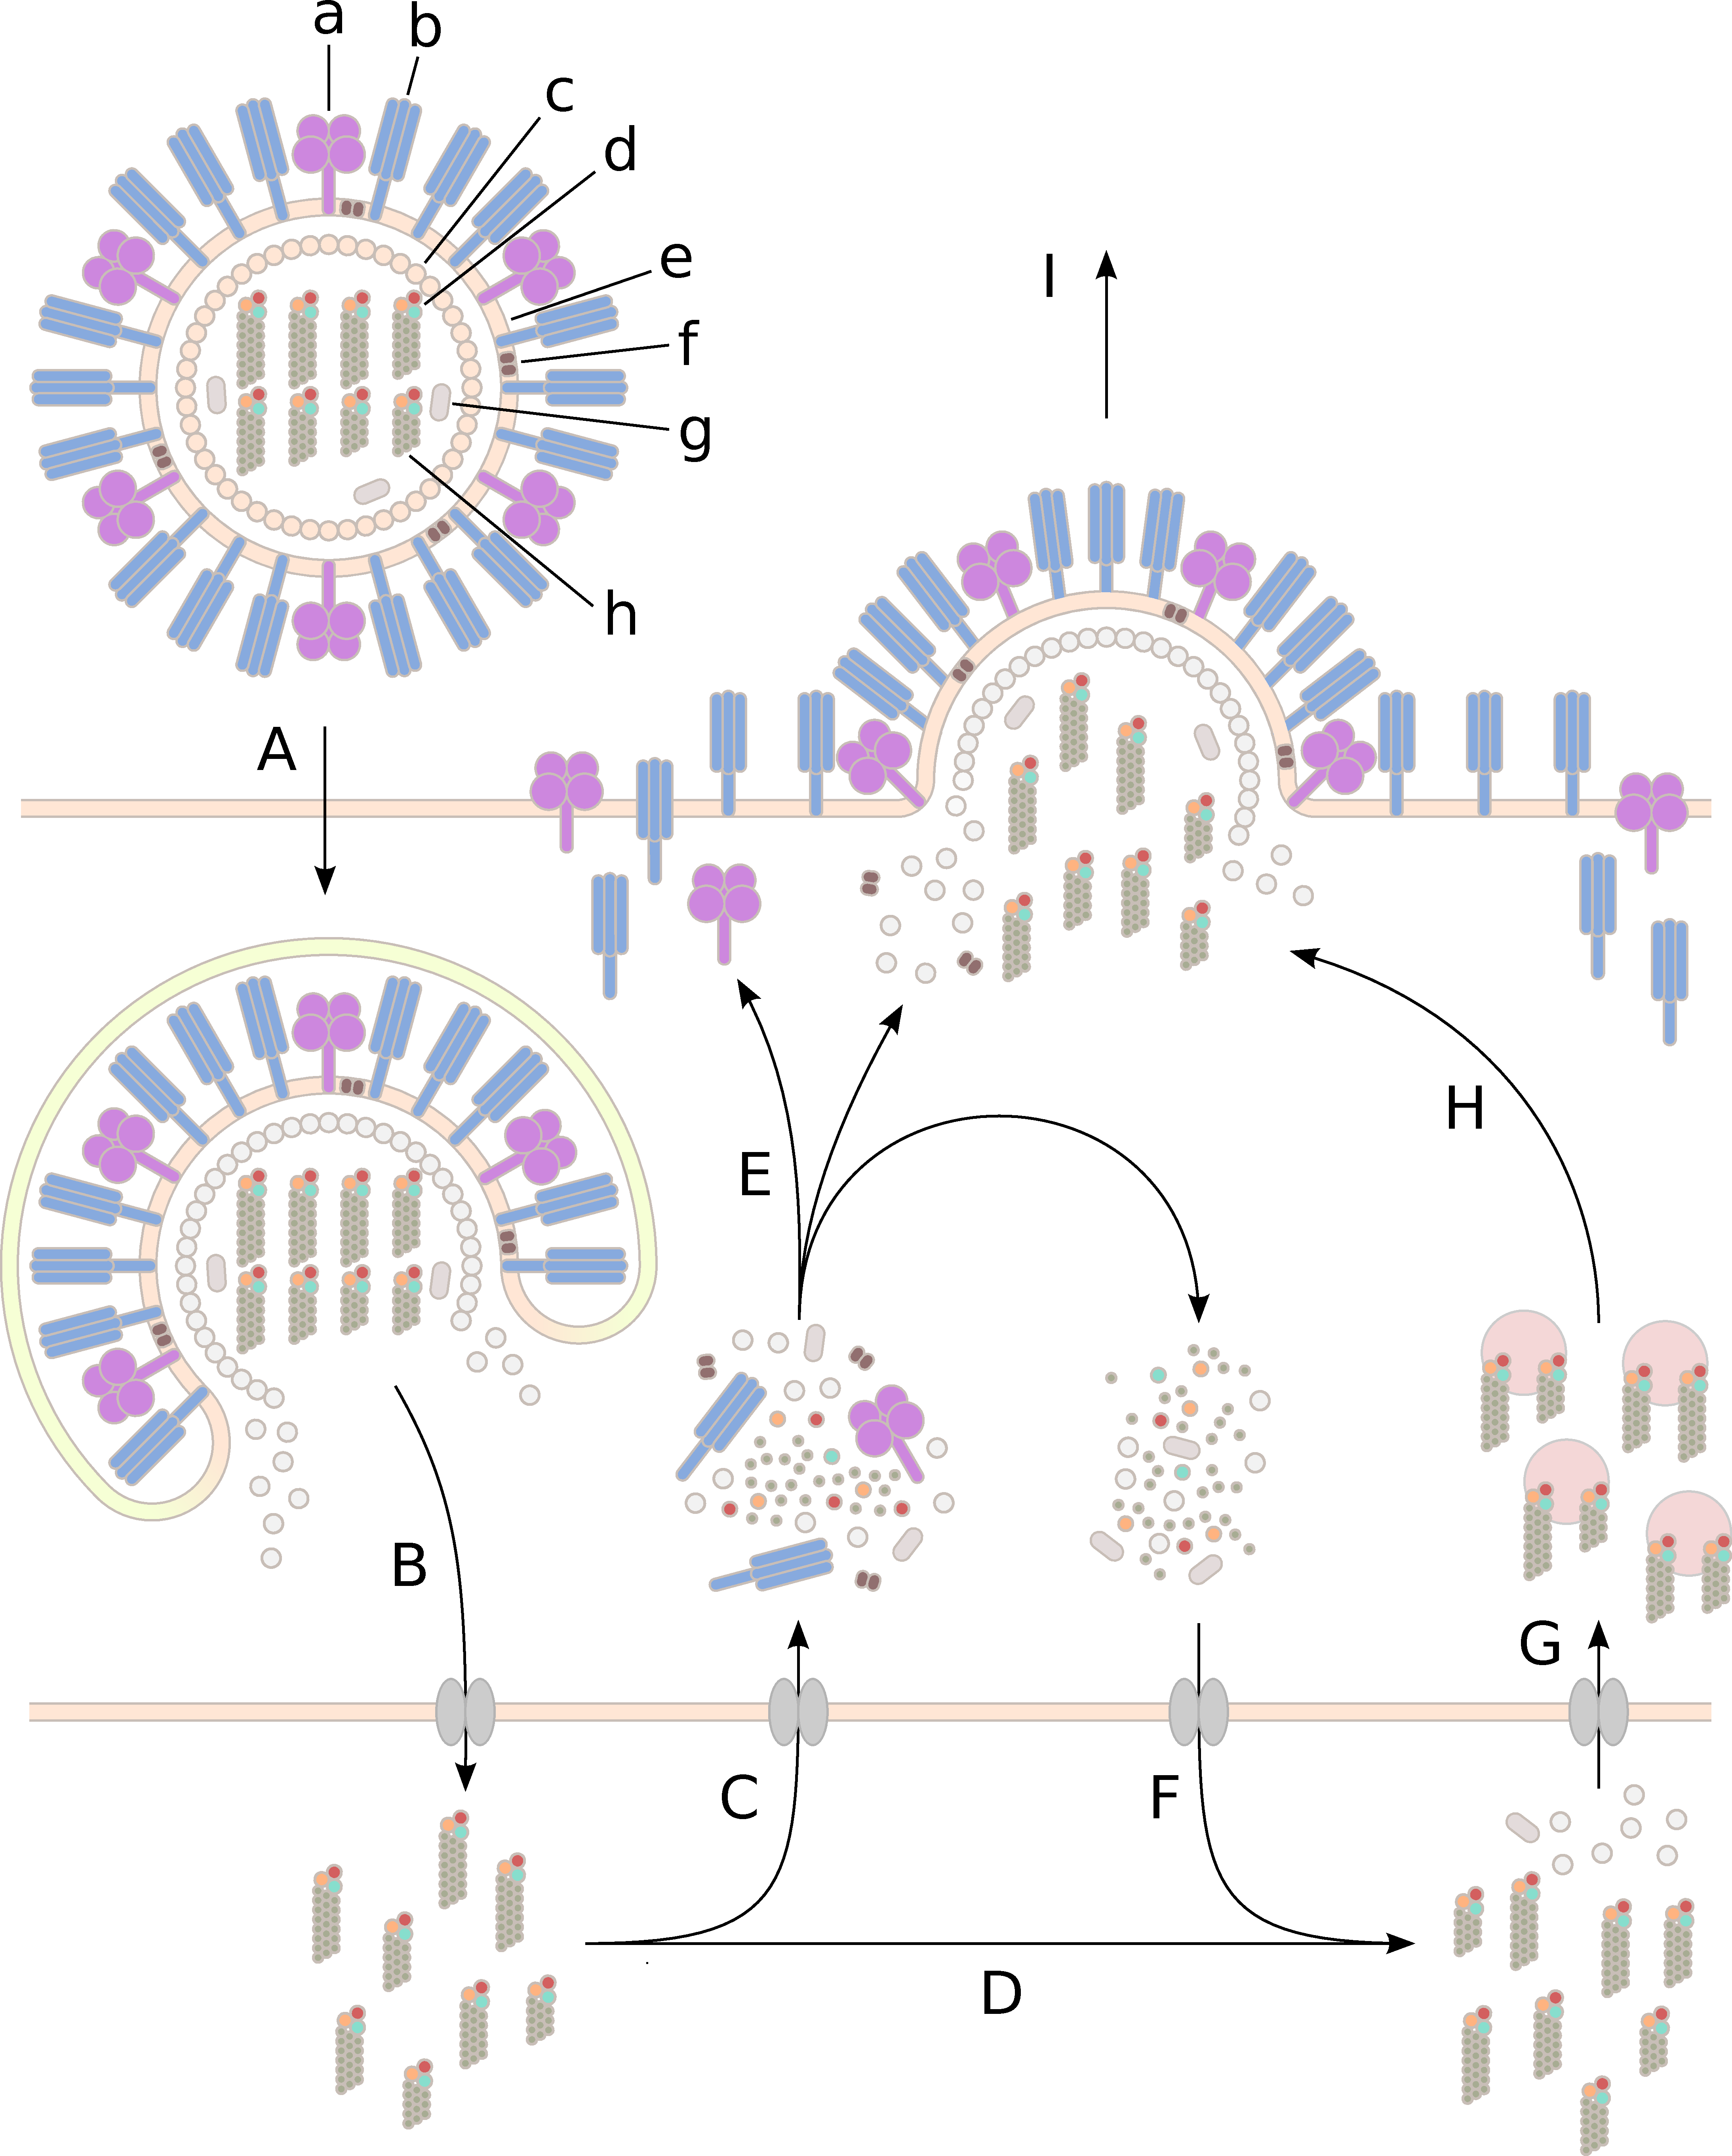
\includegraphics[width=\textwidth]{Graphics/cycle.pdf}
    \caption[\textit{Influenza A Virus} life-cycle]{\textbf{\textit{Influenza A Virus} life-cycle.} The \gls{IAV} virion attaches itself to the host cell membrane using \gls{HA} (\textsf{\textbf{a}}) to bind to the cell receptors (\textsf{\textbf{i}}). By endocytosis (\textsf{\textbf{A}}), the virion infiltrates the host cell. After assimilation into the cell, the virion escapes the endosome (\textsf{\textbf{j}}) by raising the pH involving the \acrshort{M2} protein (\textsf{\textbf{f}}), spilling the segments of the virus into the cytoplasm. After nuclear import (\textsf{\textbf{B}}) by the \gls{NPC} (\textsf{\textbf{k}}), the segments are transcribed and the \acrshort{mRNA} is transported to the cytoplasm for translation (\textsf{\textbf{C}}). The newly build \acrshort{M1} (\textsf{\textbf{c}}) and \acrshort{NEP} (\textsf{\textbf{g}}) proteins, as well as the \acrshortpl{NP} (\textsf{\textbf{h}}) and the proteins of the polymerase complex (\textsf{\textbf{d}}) are transported back into the nucleus (\textsf{\textbf{F}}) to create new \acrshortpl{RNP} with the replicated genomes (\textsf{\textbf{D}}) and enable the nuclear exit (\textsf{\textbf{G}}). The newly build \acrshort{HA}, \acrshort{NA} (\textsf{\textbf{b}}) and \acrshort{M2} proteins are incorporated into the hosts cell membrane (\textsf{\textbf{E}}). Using vesicle transport, the \acrshortpl{RNP} are transported to the position in the membrane containing the surface proteins and are incorporated into the progeny virion by embedding into \acrshort{M1} proteins (\textsf{\textbf{H}}). The virion is released involving \acrshort{NA} and \acrshort{M2} by budding the hosts cell membrane (\textsf{\textbf{I}}) and coating itself in it (\textsf{\textbf{e}}).}
    \label{fig:Cycle}
\end{figure}

% \begin{figure}
%     \centering
%     %\begin{adjustbox}{minipage=\dimexpr\textwidth-2\fboxsep-2\fboxrule,fbox}
%     \begin{subfigure}[b]{0.475\textwidth}
%         \caption[\textit{Alphainfluenzavirus}]{\textbf{\textit{Alphainfluenzavirus}}}
%         \label{subfig:Influenza_A}
%         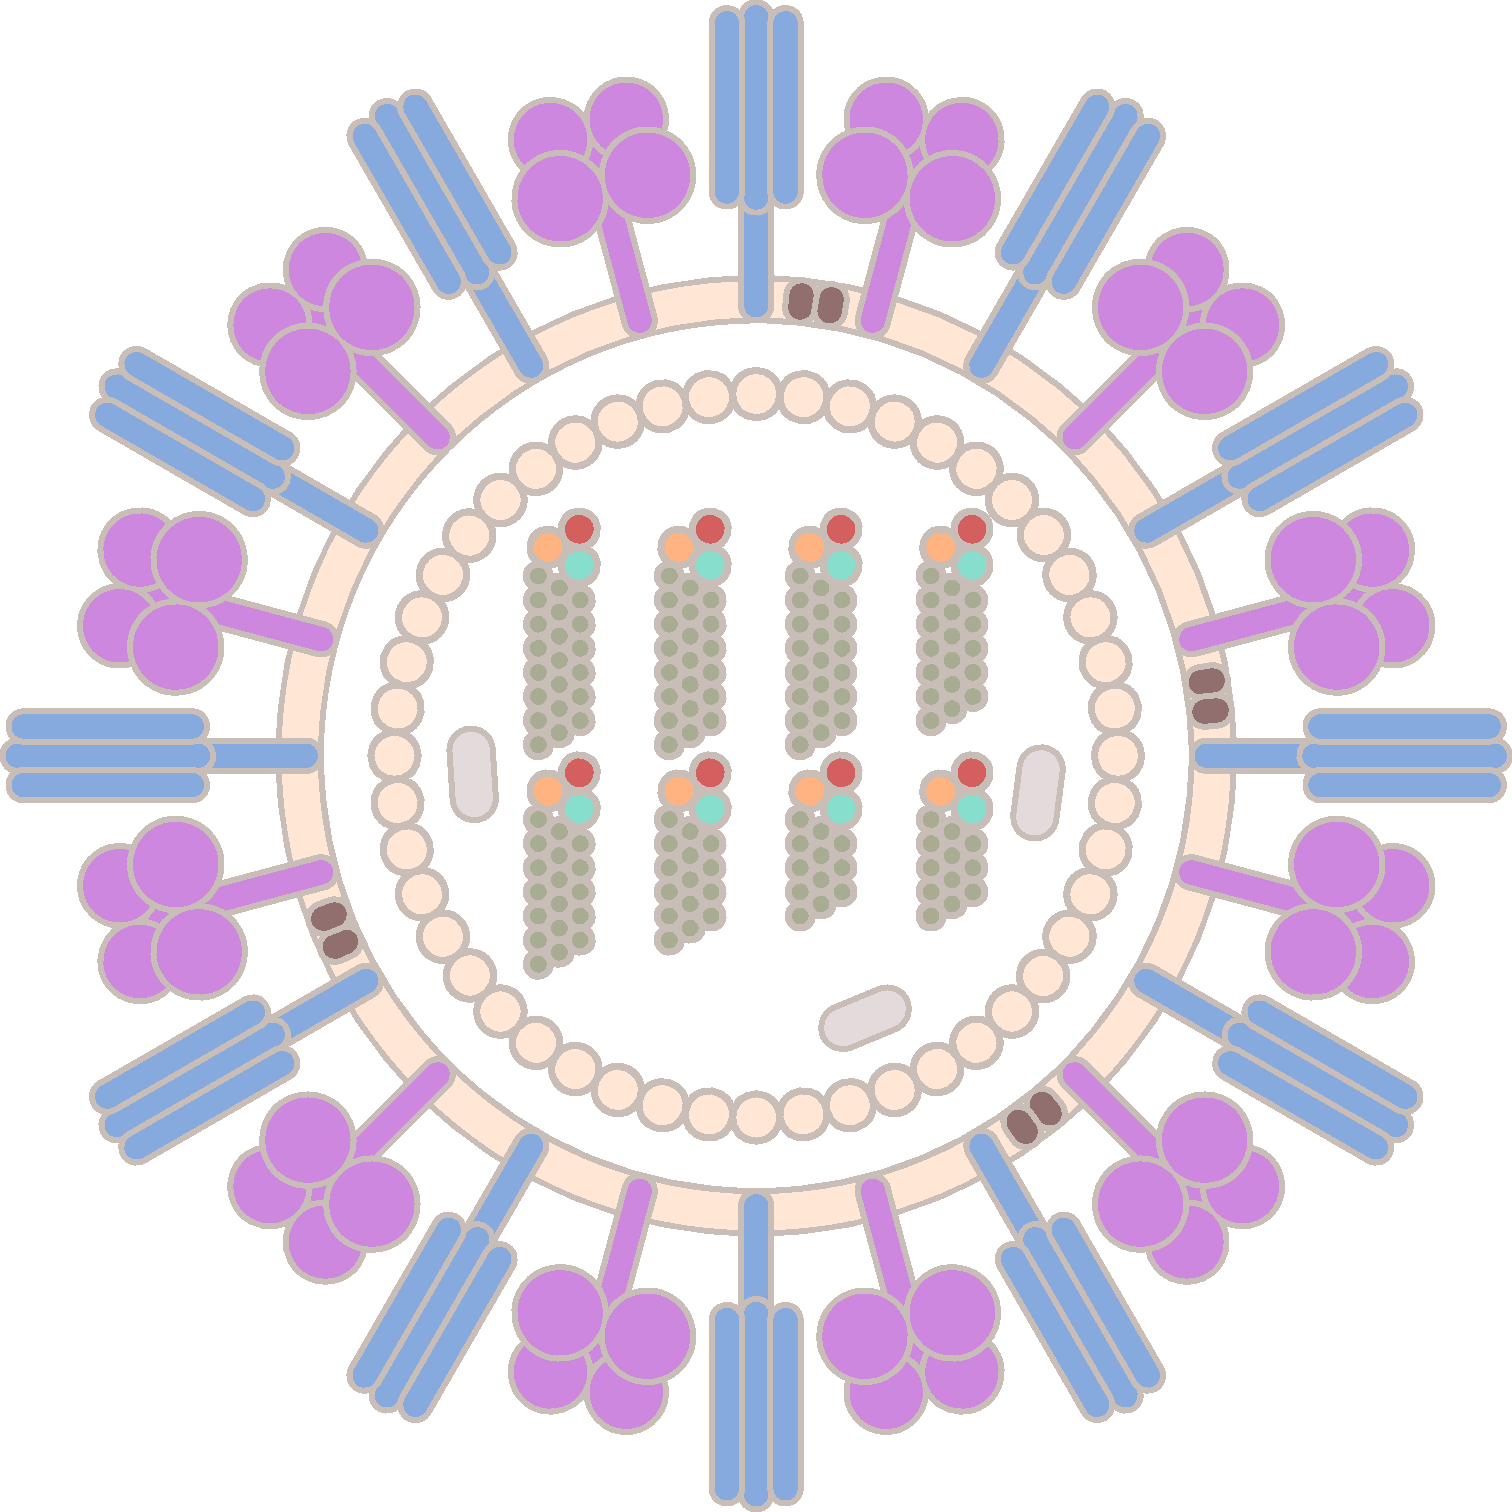
\includegraphics[width=\textwidth]{Graphics/Influenza_A.pdf}
%     \end{subfigure}
%     \hfill
%     \begin{subfigure}[b]{0.475\textwidth}
%         \caption[\textit{Betainfluenzavirus}]{\textbf{\textit{Betainfluenzavirus}}}
%         \label{subfig:Influenza_B}
%         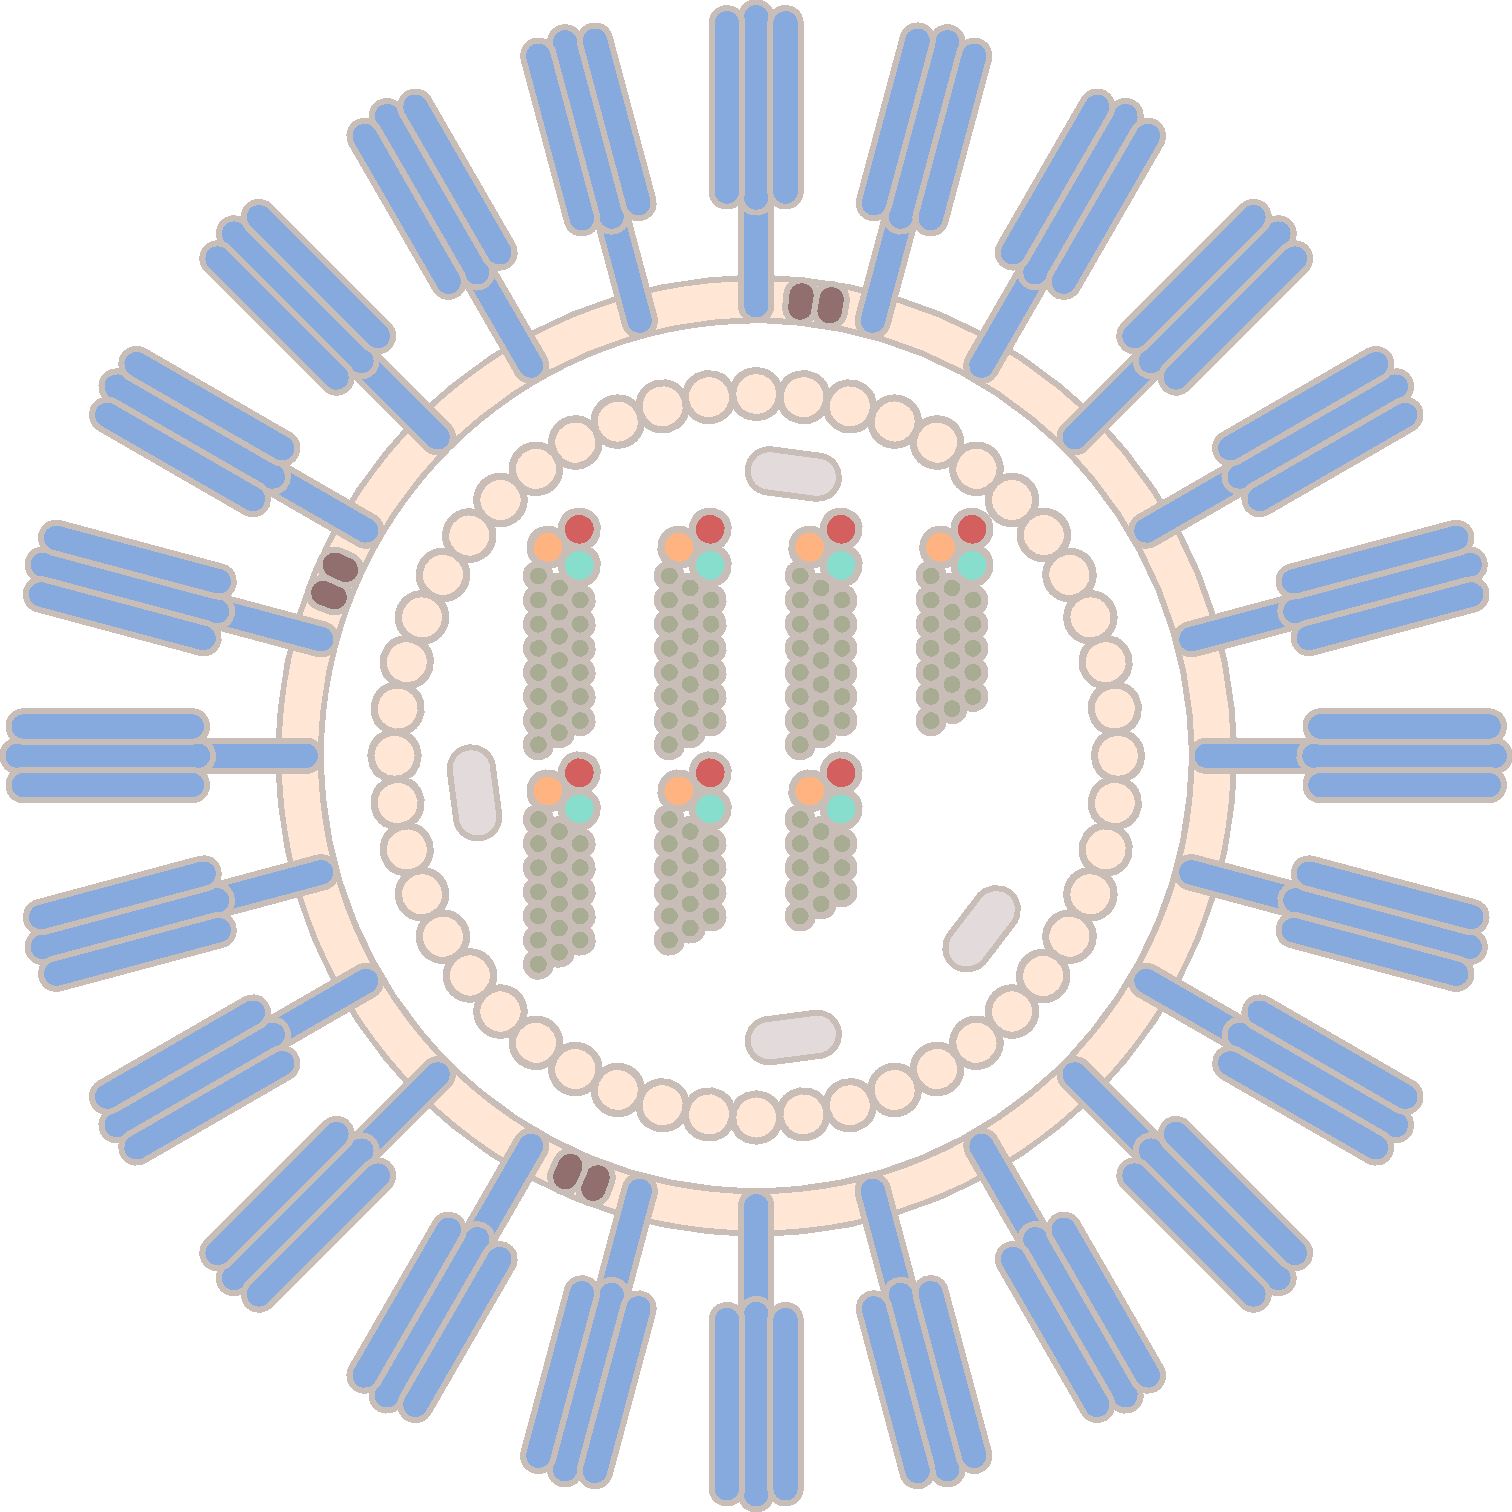
\includegraphics[width=\textwidth]{Graphics/Influenza_B.pdf}
%     \end{subfigure}
%     %\end{adjustbox}
%     \caption[\textit{Orthomyxoviridae}]{\textbf{\textit{Orthomyxoviridae}.} .}
%     \label{fig:Orthomyxoviridae}
% \end{figure}


\section{Evolution of the \textit{Influenza A Virus}}

Present day research, indicate mallards \textit{(Anas platyrhynchos)} as main reservoir and natural host of \glspl{LPAIV} \autocite{jourdain_influenza_2010}. Studies on Pekin ducks, descended from mallards, have shown minor immune responses and antibody production to the infection with \gls{IAV} strains and the possibility of a reinfection after two months with the same strain \autocite{kida_duck_1980}. Strains are lines of \gls{IAV} related to a specific location and time point \autocite{cann_chapter_2016}. Less dangerous strains of \gls{IAV}, called \glspl{LPAIV}, seem to repeatedly circulate in duck species and may evolve into human pathogenic strains by zoonoses \autocite{jourdain_influenza_2010}. Simple transmission over species is not enough to start a pandemic though, therefore, better understanding of the mostly unknown genetic changes vital for zoonotic events is required \autocite{van_reeth_avian_2007}. Circulation of these strains in aquatic bird species with continued evolution enable the transmission possibilities to humans, lower animals, and other birds \autocite{webster_chapter_1999}. The evolution occurs in all segments of the \gls{IAV} but is most prominent in \gls{HA} and \gls{NA} \autocite{webster_chapter_1999}. Infection is mostly dependent on these surface glycoproteins, or surface antigens as they are crucial for antigenic attachment to host cells \autocite{cann_chapter_2016}. Significant variation in the surface antigens mostly occur by reassortment, also called genetic shift and point mutations, also called antigenic drift \autocite{webster_chapter_1999}. Current classification of \gls{IAV} by the subtypes nomenclature is solely based on characterization of the antigens \autocite{noauthor_revision_1980}. Prior to the current classification, \gls{IAV} subtypes were separated by host origin, based on defining just major antigenic differences. These previous subtypes consisting of H0 to H3, Hsw1, Heq1, Heq2 and Hav1 to Hav10 were replaced by the known subtypes H1 to H12 for \gls{HA} and in a similar similar for \gls{NA} by replacement of N1, N2, Neq1, Neq2 and Nav1 to Nav6 in favor of N1 to N9 \autocite{noauthor_revised_1971}. The subtype nomenclature was changed to include more subtle characterization of the \gls{IAV} genome based on immunological relationships \autocite{noauthor_reconsideration_1979}. Thereby, the \gls{IAV} subtypes were described by a sequential system involving the antigenic character regardless of host origin. Origin and other informations are included in the strain naming system involving position, number and year of detection \autocite{noauthor_revision_1980}. The current subtypes were also grouped according to the sequence homology of the \gls{NS1} with some major differences \autocite{noauthor_reconsideration_1979}. Still, due to missing serological data for \gls{NS1}, only \gls{HA} and \gls{NA} were used for the classification. Other segments were not considered due to being highly conserved \autocite{noauthor_reconsideration_1979}. However, future classification involving all the segments was not negated, if appropriate \autocite{noauthor_reconsideration_1979}. %Subtype convention on the surface proteins was, therefore, agreed due to low conservation because of high evolutionary pressure.

\vspace{1em}

Point mutations in the segmented genome are very frequent, as the mutation rate in all RNA viruses is very high \autocite{duffy_why_2018}. Present \textit{poliovirus} research, indicate higher selection for faster replication and, therefore, acceptance of replication errors in favor of faster viral polymerases \autocite{pfeiffer_increased_2005, duffy_why_2018}. This finding is in line with research indicating the short length or segmentation of RNA viruses and the high mutation rates as evolutionary trade-off \autocite{belshaw_pacing_2008, vignuzzi_closing_2012}. Thereby, creating a cloud of offsprings, called quasispecies, with 1-2 mutations in the genome each \autocite{belshaw_pacing_2008, vignuzzi_closing_2012}. The point mutations can affect the offsprings proteins \gls{AA} composition in the translation process, by possible missense and nonsense errors or frameshifts \autocite{parker_errors_1989, webster_chapter_1999}. 

\FloatBarrier

Reassortment is a more drastical change in the surface proteins and likely to be related to the pasts most horrible \gls{IAV} pandemic, the spanish flu in 1918 \autocite{nelson_multiple_2008}. For reassortment induced zoonoses, there practically always has to be a intermediate host or \glqq mixing vessel\grqq{}, most likely pigs, able to be infected by \glspl{IAV} strains of different hosts origin \autocite{shu_evidence_1994}. The hosts cells can then be co-infected by two different \glspl{IAV} and create offsprings with mixed segments \autocite{compans_influenza_2014}. All segments can be exchanged, but, in case of surface proteins of different hosts, \glspl{IAV} can occur that are able to do interspecies transmission \autocite{shu_evidence_1994}. Avian \gls{IAV} strains can, thereby, evolve to human strains by co-infection of a pig with human transferable and avian originating \gls{IAV} strains \autocite{shu_evidence_1994}. 

\section{Vaccines design and the link to reassortment}

Reassortment events are a major source of danger, since no real cure to \gls{IAV} infection is available and generation of vaccines is straining and not always as effective as expected \autocite{wahlgren_influenza_2011, wong_traditional_2013}. Furthermore, the efficacy of vaccines vary in specific populations and there are limitations to the manufacturing and the time frame of the production \autocite{wong_traditional_2013}. The strains most likely to circulate for the season are selected twice a year by the \gls{WHO}, to be included in vaccines prepared for the winters in both hemispheres \autocite{barr_epidemiological_2010}. The seasonal used \gls{IAV} vaccines target the highly mutable head domain of \gls{HA} surface proteins to stimulate immune response \autocite{wong_traditional_2013, wei_next-generation_2020}. Therefore, the \gls{IAV} vaccines efficiency vary depending on the similarity of the \gls{HA} head domain of the strains used for the vaccines and the ones circulating in the season \autocite{wei_next-generation_2020}. The accuracy of the recommendation by the \gls{WHO} is, therefore, especially crucial for the survival of humans with pre-existing conditions or humans of old age that are more prone to infection. To manufacture the vaccines, reassortment of the selected strain with a master strain is induced in eggs \autocite{wong_traditional_2013}. The resulting hybrid strain contains the selected strains surface proteins and the master strains high-growth properties necessary for production of the vaccine in the short time frame \autocite{wong_traditional_2013}. Therefore enlarging the knowledge of \gls{IAV} reassortment is important for the prediction of future pandemic strains, creation of vaccines by high-growth hybrid strains and the overall efficiency of the vaccines against circulating variable strains most likely to undergo reassortment \autocite{wong_traditional_2013, dadonaite_structure_2019}. For better understanding of \glspl{IAV} reassortment and estimation of resulting risks, the interaction mechanisms of the genome segments have to be fully discovered \autocite{dadonaite_structure_2019}. 

\section{Importance of secondary structure predictions}

The eight \gls{IAV} \gls{ssRNA} segments are single-stranded chains of nucleotides, by inter- and intra-molecular base-pairing various complex arrangements with different stabilities can be build \autocite{higgs_rna_2000, dadonaite_structure_2019}. Single-stranded RNA viruses can use secondary structures on the \gls{ssRNA} as well as on the transcribed positive \gls{mRNA} for different mechanisms, like the initiation of the translation on the \gls{mRNA} by the \gls{IRES} \autocite{kieft_viral_2008}. Segmented viruses are able to perform inter-molecular binding of different \gls{ssRNA} segments to each other \autocite{moss_identification_2011, dadonaite_structure_2019}. \textcite{gerber_selective_2014} described the selective \glspl{IAV} packaging by segment interactions with consequences for reassortment. It is assumed, that different interactions favor reassortment while others prevent specific segment incorporation in the reassortant virus. Fully understanding the conserved structures and interactions of \glspl{IAV} segments would, thereby, enlarge our knowledge of \gls{IAV} to a great extend. Prediction of these viral secondary structures is mostly done by lab methods \textit{in virio} and \textit{in vitro} or computationally with \textit{in silico} methods, with the latter mostly based on thermodynamic calculations alone \autocite{moss_identification_2011, dadonaite_structure_2019}. \textit{In virio} methods involve modification inside a virion and \textit{in vitro} methods involve modification on transcribed RNA in a probe, both can used with SHAPE-MaP and SPLASH methods \autocite{smola_selective_2015, dadonaite_structure_2019}. Following the lab methods structure prediction is performed by tools using the insight of the lab methods for better accuracy, in \textcite{dadonaite_structure_2019} using \texttt{IntaRNA} \autocite{mann_intarna_2017}. Prediction of present day secondary structures by \textit{in silico} thermodynamic energy minimization calculations is mostly performed by tools involving the ViennaRNA package and, on single sequences, by \texttt{RNAfold} \autocite{lorenz_viennarna_2011}. Both lab methods can only be used to analyze secondary structure folding on single viruses at once, but reveal structures at single-nucleotide resolution \autocite{dadonaite_structure_2019}. \textit{In silico} methods that are used without support by experiments are not limited by prediction on single viruses, only require prior sequenced genomes \autocite{moss_identification_2011, dadonaite_structure_2019}. Since \textit{in silico} methods can be used on a higher number of sequences at once, consensus structures can be predicted together to find conserved, possibly equal folding regions in the sequenced genomes by prior multiple sequence alignments \autocite{moss_identification_2011}. 

\section{Alignments and clustering}

Aligning multiple sequences to each other is possible by a number of different methods nowadays. The core of most multiple alignment methods were created by \textcite{needleman_general_1970} with an algorithm usable to aligns two sequences in a pairwise manner using fast dynamic programming. The algorithm was intended to be used solely on proteins but could be transfered to any problems involving pairwise distance and was soon used for nucleotide sequence comparisons \autocite{phillips_multiple_2000}. Other algorithms were created in the following years but the one proposed by Needleman and Wunsch was soon used to not only align two sequences but multiple sequences creating the possibility sequence comparisons of multiple sequences \autocite{phillips_multiple_2000}. Due to inability to be used on high numbers of sequences other algorithms, like the one proposed by \textcite{feng_progressive_1987}, were created that did not offer the same accuracy but could be performed on higher number of sequences, thereby, creating first heuristic multiple sequence alignment methods. The way for present multiple sequence alignments was paved, offering the possibility to align higher numbers of sequences in reasonable time. Present day multiple alignment tools offering global comparisons of the complete sequences are still based on these heuristic methods. Famous ones are up-to-date versions of \texttt{CLUSTALW} first proposed in \textcite{thompson_clustal_1994} and \texttt{T-COFFEE} proposed in \textcite{notredame_t-coffee_2000}. While steps in terms of accuracy had been made in the development of newer versions, calculations still have high CPU times and hardware offering high amounts of computational power are still needed \autocite{katoh_mafft_2002}. Other alignment methods exist searching for similar short profiles in the sequences and extend these matches. \texttt{MAFFT} first proposed in \textcite{katoh_mafft_2002} and evolved to the present day version as described in \textcite{katoh_mafft_2013} uses \gls{FFT} for similar profile search, resulting in faster and less costly nucleotide sequence comparison. \texttt{MUSCLE} also prominent for \glspl{MSA} creation is based on $k$-mers profiles instead, also improving speed \autocite{edgar_muscle_2004}. Higher numbers of aligned in shorter time-spans enable searching for conserved structures in a higher magnitude. \glspl{MSA} created by the available present day tools can be used in structure predictions by e.~g.~, \texttt{RNAalifold} \autocite{bernhart_rnaalifold_2008}.

\begin{figure}[!hbt]
    \centering
    %\begin{adjustbox}{minipage=\dimexpr\textwidth-2\fboxsep-2\fboxrule,fbox}
    \begin{subfigure}[b]{0.475\textwidth}
        \caption[Compactness]{\textbf{Compactness}}
        \label{subfig:Compactness}            
        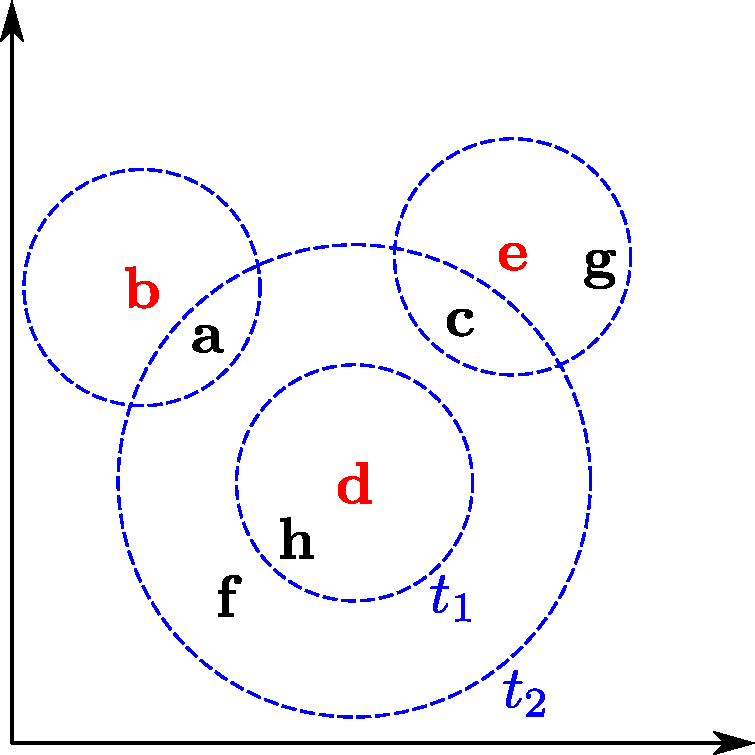
\includegraphics[width=\textwidth]{Graphics/Compactness.pdf}
    \end{subfigure}
    \hfill
    \begin{subfigure}[b]{0.475\textwidth}
        \caption[Connectedness]{\textbf{Connectedness}}
        \label{subfig:Connectedness}            
        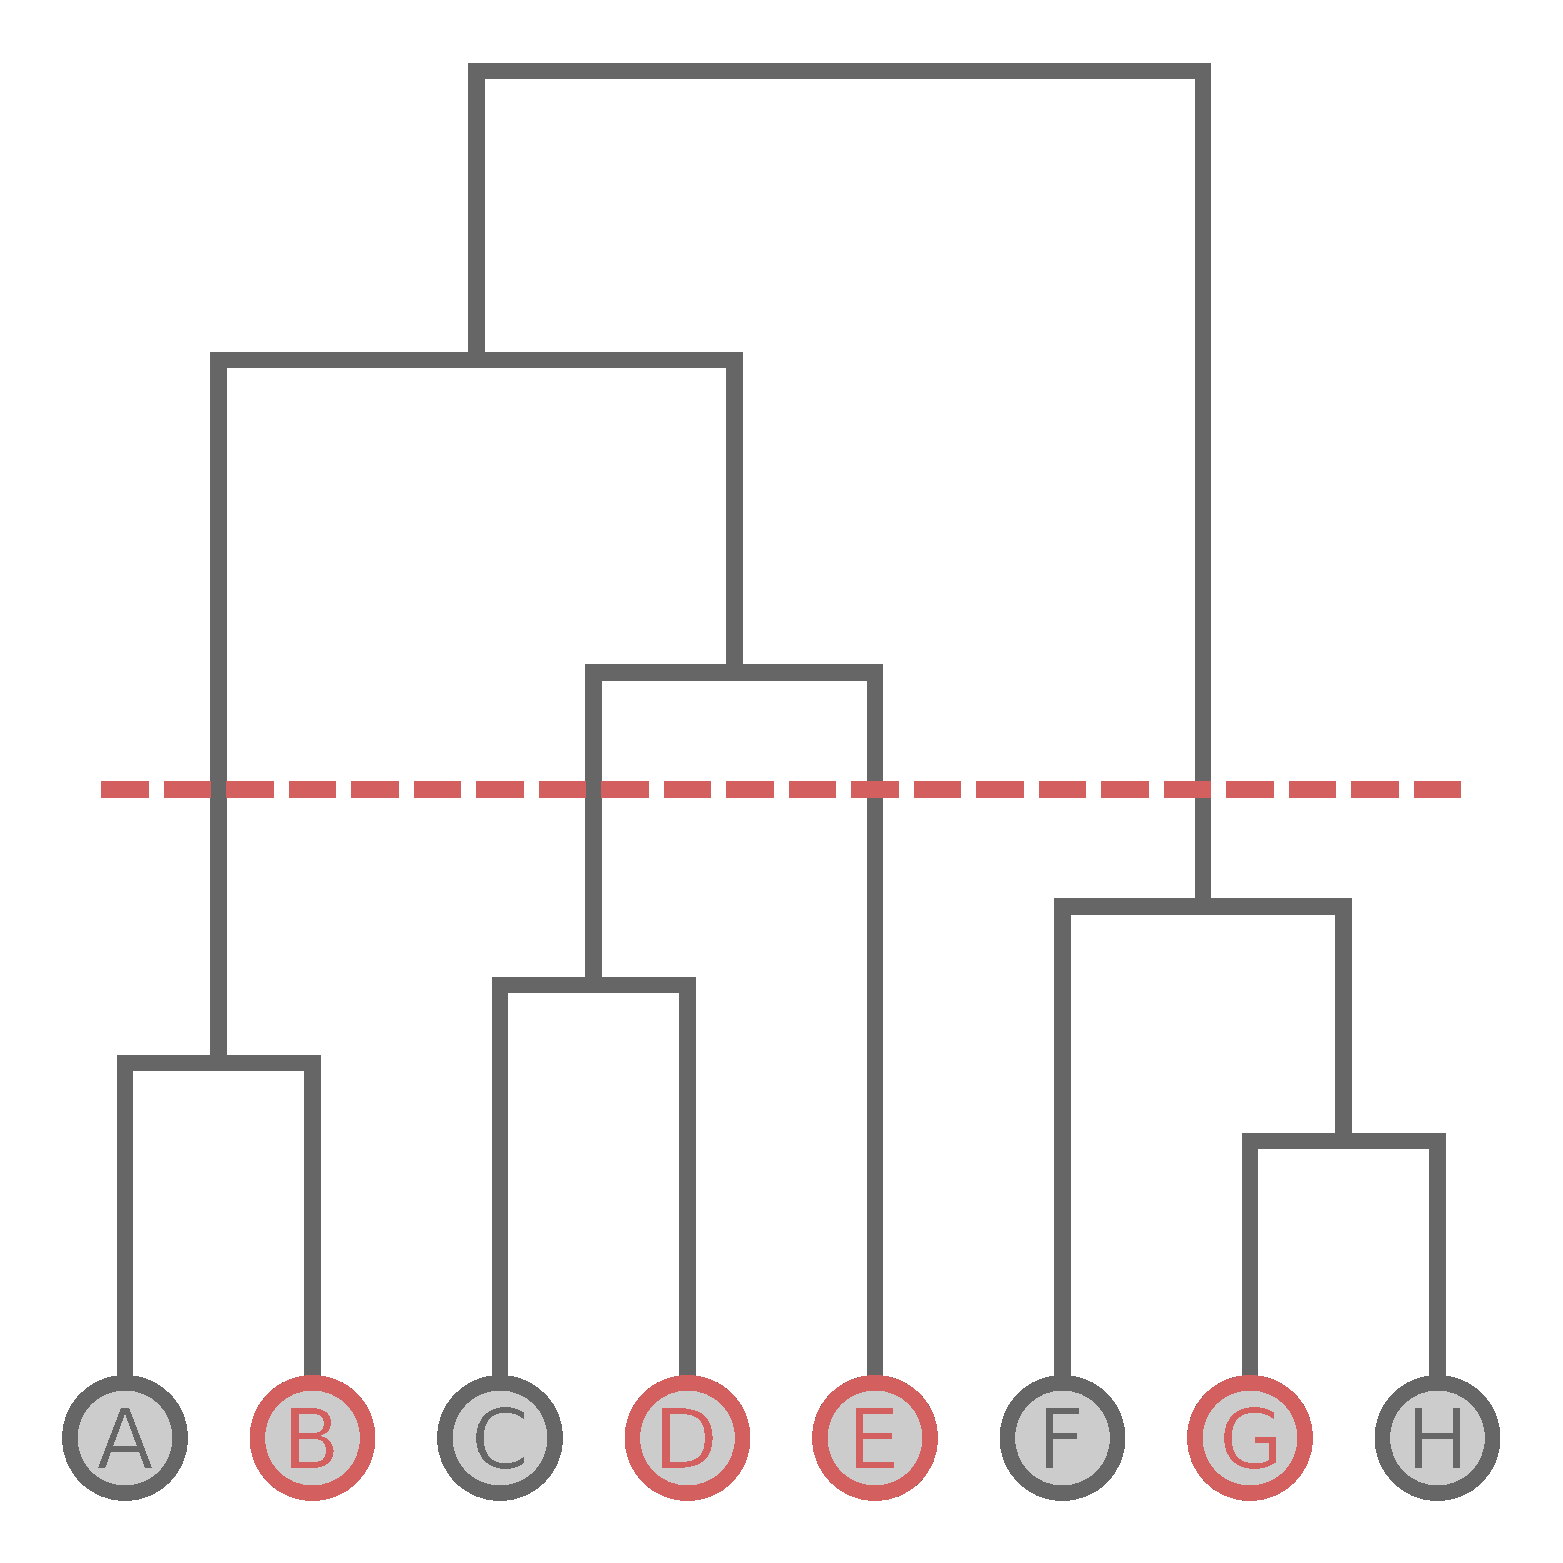
\includegraphics[width=\textwidth]{Graphics/Connectedness.pdf}
    \end{subfigure}
    %\end{adjustbox}
    \caption[Clustering methods]{\textbf{Clustering methods.} Clustering is most frequently used by density-based separation using the compactness concept or agglomerative hierarchical clustering with the connectedness concept. The letters denote datapoints with the clusters most meaningful points as centroids in red, when using threshold $t_1$. Both methods are highly dependent on the used parameters for the clustering. Therefore, the thresholds $t_1$ and $t_2$ illustrate major differences on the resulting clustering. Choosing $t_1$ or $t_2$ in the hierarchical connectedness clustering either produce a cluster containing c, d and e or two clusters one containing c and d the other containing only e, resulting in unclustered e. Setting the threshold to high can on the other hand result in a even smaller number of large clusters containing higher differences. Setting the value to small results in more unclustered datapoints. Threshold definition in the density-based compactness clustering defines the magnitude of the density necessary to induce cluster separation. For the illustration of the compactness clustering the values for $t_1$ and $t_2$ are used as cluster selection by a  radius including at least a number of two points in it for $t_1$ and five points for $t_2$. Therefore, $t_1$ would create three clusters leaving f out unclustered. The value $t_2$ on the other hand would create a bigger cluster with higher differences, including f but would most likely leave b e and g unclustered.}
    \label{fig:Methods}
\end{figure}

\vspace{1em}

Since \textit{in silico} methods are based on sole predictions involving thermodynamic calculations, the choice of a set to use when aiming to make statements about higher amounts of sequences is crucial. Prediction of conserved consensus structures is, therefore, highly fragile in terms of high genomic differences of the used sequences. Prior clustering to discover related groups can be helpful in improving the accuracy of consensus structures as performed in \textcite{moss_identification_2011} for prediction of a tetraloop structure. Clustering techniques are broadly used to discover new insights of biological data, not only to predict more accurate structures in \gls{IAV} segments, but also to be used on post-genomic data in all fields of bioinformatics knowledge\autocite{handl_computational_2005}. Clustering methods exist based on entirely different concepts to separate the data. They can split given data in groups by connectedness, compactness or spatial separation of data points \autocite{handl_computational_2005}. By separation based on compactness, the method aims to reduce the intra-cluster variation as much as possible, thereby, mostly creating spherical clusters (\autoref{subfig:Compactness}) \autocite{handl_computational_2005}. The concept of connectedness connects neighbors to each other, thus, creating chains of associated data points (\autoref{subfig:Connectedness}). The clusters are mostly arbitrarily shaped. Spatial separation is a concept aiming for splitting the data in different regions and is related to the concept of connectedness \autocite{handl_computational_2005}. Existing clustering algorithms try to best separate the data based on these concepts. Still, no existing clustering algorithm can take all of these concepts into consideration. Most clustering algorithms follow the principle of either connectedness, like hierarchical clustering algorithms, or the compactness concept, involving also the spatial separation, like density-based clustering algorithms \autocite{handl_computational_2005}. Hierarchical clustering algorithms can be used by starting with each datapoint in a single cluster and merging while climbing the hierachy, called agglomerative or divisive, when starting in on cluster and dividing in smaller ones \autocite{murtagh_algorithms_2012}. Prominent widely used examples for agglomerative hierarchical clustering are the \gls{UPGMA} method, that is also present in \texttt{MAFFT} for guide tree creation or the recent published \texttt{HDBCSCAN} tool using the single-linkage  method \autocite{katoh_mafft_2002, mcinnes_hdbscan_2017}. A well-known examples for density-based clustering is the tool \texttt{DBSCAN} \autocite{madhulatha_overview_2012, schubert_dbscan_2017}. Regardless of which clustering methods is used, there is always a threshold that has to be defined in order for the algorithm to work as expected (\autoref{subfig:Connectedness}) \autocite{madhulatha_overview_2012}. Visual inspection on the clustering is not always possible making these threshold parameters a tough choice. Hierarchical clustering methods need a threshold to define the cutoff in the tree and density-based methods depend on choosing the size of an area with a given density to be handled as cluster \autocite{madhulatha_overview_2012}. Estimation of a reasoned number of clusters is possible in hierarchical clustering methods by the elbow method, thus, reverse estimating the threshold parameter necessary for the number of clusters \autocite{satopaa_finding_2011, madhulatha_overview_2012}. Clustering methods, like \texttt{USEARCH} and \texttt{CD-HIT}, that are especially developed to be used for sequence clustering, require a threshold based on sequence similarity only \autocite{li_cd-hit_2006, edgar_usearch_2010}. However, the majority of cluster tool use data points as vectors for clustering in statistical data analysis and distance measurements in instead of sequence similarity \autocite{madhulatha_overview_2012}. The dimensionality of these vectors is dependent on the amount of information. Using vectors with a high amount of information for clustering requires lowering the dimensionality of the data prior to clustering \autocite{assent_clustering_2012}. Therefore, combination of the clustering with methods, that reduce dimensionality is crucial in the most cases. Widely used methods for reducing the dimensionality of vectors are \texttt{PCA}, \texttt{t-SNE} and \texttt{UMAP}. Choosing the right amount of preserved information in combination with wisely selected thresholds define, thus, a well conducted high-dimensional vector clustering. 

\section{The proposed project}

The present subtype classification of \gls{IAV} is solely based on immunological research on the surface proteins. Since release of this classification around 40 years, with enormous progress in computer technology, have passed. Aside from the raw number of new sequenced genomes of \gls{IAV} in these years, also ways for faster sequence comparisons methods using profiles like $k$-mer comparisons and more accurate clustering algorithms were paved. Using knowledge from this elapsed time, the current classification will be reevaluated from the perspective of bioinformatics, to possibly find subtle differences to renew the classification with more detailed subgroups \autocite{noauthor_revision_1980}. Due to the usage of the raw amount of all high quality sequences available for \gls{IAV}, the clustering into groups were performed without any alignments, searching for a faster, more scaleable and hopefully more accurate method. Instead of alignments a distance measurement using vector representation based on genomic $k$-mers will be used in combination with high dimensional clustering methods. As already mentioned $k$-mer distance for genomic comparison was also described in \textcite{edgar_muscle_2004} for faster alignments. To handle the high dimensionality of the used $k$-mer representation vectors used in this project, different dimension reduction methods were described and compared. For clustering hybrid \texttt{HDBSCAN} will be used combining compactness and connectedness for the best accuracy possible aiming for high quality clustering of the huge amount of highly variable \gls{IAV} sequences. Threshold definition is a complex procedure with high impact on the results and will be solved by different approaches involving the Kneedle Algorithm implementing the elbow method for the most appropriate results. This project aims for a clustering based classification of all eight segments of \gls{IAV}, hopefully paving the way for future research to discover more detailed consensus structures and new insights into the molecular life-cycle of the \gls{IAV}. The current subtype classification will support the clustering of segment 4 \gls{HA} in this project and, thereby, create a blueprint to cluster the other segments in a similar way. Nevertheless, due to the lower evolutionary pressure less clusters for the segments not coding for surface proteins are to be expected. For a simple usable new classification, less than 100 clusters per segment would be comfortable and are anticipated, when considering the number of reassortment events in H1N1 proposed in \textcite{nelson_multiple_2008}. 

%\section{WHO classification of \textit{Influenza A Virus}}

%The present day classification of \gls{IAV} is based on the serotype of the virus 

%hybrid clustering combianing both concepts!!

%develop no einteilung sinnvoll fpr secondarys 

%centroid sequences

%To test whether a subset of sequences prefers the tetraloop structure, sequences were clustered using the Unweighted Pair Group Method with Arithmetic Mean (UPGMA)

%To increase the overall efficiency, strategies of next-generation vaccines focus on less variable structures of \gls{HA} and other \gls{IAV} proteins, namely \gls{NA}, \gls{M2} and the \glspl{NP} \autocite{wei_next-generation_2020}. Predicting the overall structure of the \gls{IAV} segments, that are crucial for the virus survival are, thus, essential for drug and vaccine creation against \gls{IAV} and still 

%expected are so und so viele based on the evol variation in dem nature paper wo es nur um H1 ging blabla 1-10 cluster pro subtype

% hierarchical clustering \autocite{gower_minimum_1969}. 

% \blindtext

% \blindtext

% \begin{figure}
%     \centering
%     %\begin{adjustbox}{minipage=\dimexpr\textwidth-2\fboxsep-2\fboxrule,fbox}
%     \begin{subfigure}[b]{0.475\textwidth}
%         \caption[Euclidean]{\textbf{Euclidean}}
%         \label{subfig:Euclidean}
%         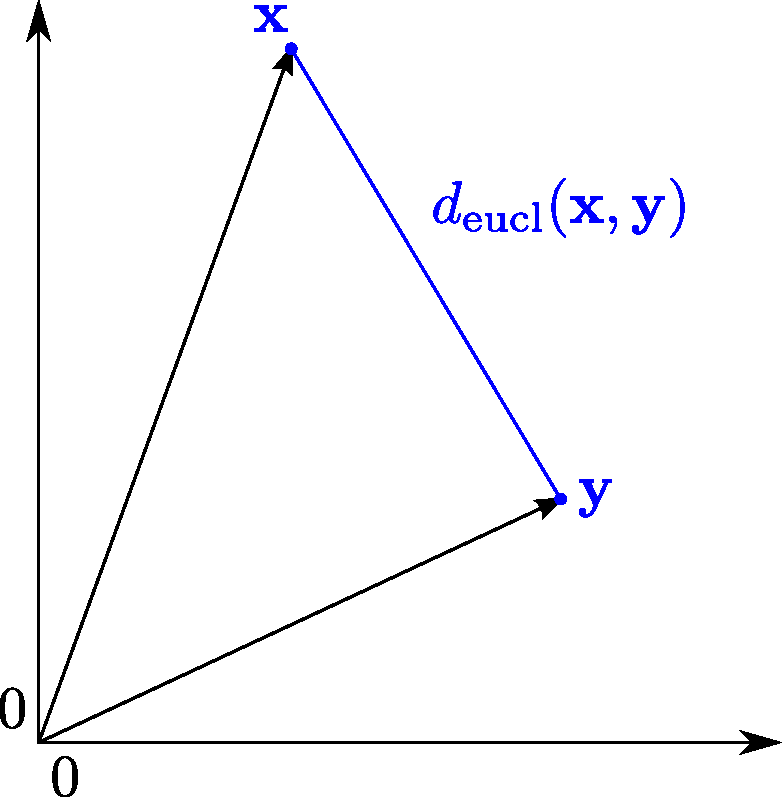
\includegraphics[width=\textwidth]{Graphics/Euclidean.pdf}
%     \end{subfigure}
%     \hfill
%     \begin{subfigure}[b]{0.475\textwidth}
%         \caption[Cosine]{\textbf{Cosine}}
%         \label{subfig:Cosinus}            
%         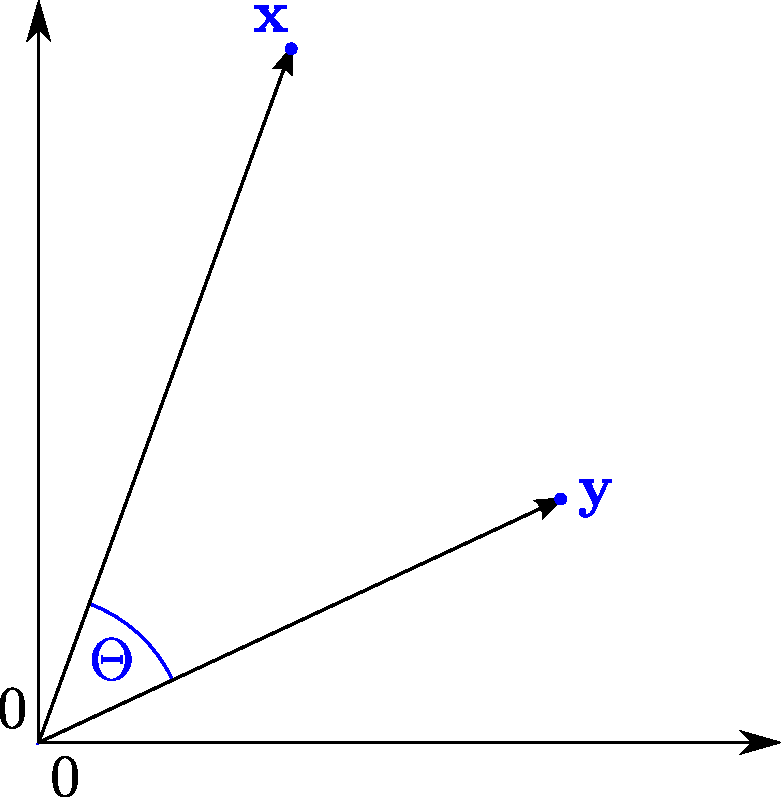
\includegraphics[width=\textwidth]{Graphics/Cosinus.pdf}
%     \end{subfigure}
%     %\end{adjustbox}
%     \caption[Distance Measuring Methods]{\textbf{Distance Measuring Methods.} .}
%     \label{fig:Distance}
% \end{figure}

% \blindtext

% % \begin{fequation}[!hbt]
% %     \begin{empheq}[box=\fbox]{alignat* = -1}
% %         &xL &&&&+zL &&\longrightarrow xL &&&&+zH\\
% %         &xM &&+yL &&+zH &&\longrightarrow xM &&+yL &&+zL\\
% %         &xM &&+yM &&+zL &&\longrightarrow xM &&+yM &&+zH\\
% %         &xH &&+yL &&+zH &&\longrightarrow xH &&+yL &&+zL\\
% %         &xH &&+yM &&+zH &&\longrightarrow xH &&+yM &&+zL\\
% %         & &&\hphantom{++}yH &&+zL &&\longrightarrow &&\hphantom{++}yH &&+zH
% %     \end{empheq}
% %     \caption[]{\textbf{.}}
% %     \label{gl:8.2}
% % \end{fequation}

% \textbf{Normalization with max-norm:} 
% %is the normalization so that the l2 norm of a vector is 1 !!!!!

% \begin{empheq}{alignat = -1}
%     \hat{\mathbf{x}} &= \frac{\mathbf{x}}{\Vert\mathbf{x}\Vert_{\text{max}}}
% \end{empheq}

% \begin{empheq}{alignat = -1}
%     \Vert\hat{\mathbf{x}}\Vert_{\text{max}} &= 1
% \end{empheq}

% \textbf{Cosinus similarity:}

% \begin{empheq}{alignat = -1}
%     %&\cos\angle(\mathbf{x}, \mathbf{y}) &&= \frac{\mathbf{x}^\top\mathbf{y}}{\Vert\mathbf{x}\Vert \cdot \Vert\mathbf{y}\Vert}
%     &\cos(\Theta) &&= \frac{\mathbf{x}^\top\mathbf{y}}{\Vert\mathbf{x}\Vert \cdot \Vert\mathbf{y}\Vert}
% \end{empheq}

% \textbf{cosinus distance}

% \begin{empheq}{alignat = -1}
%     %&d(\mathbf{x},\mathbf{y}) &&= 1 - \cos\angle(\mathbf{x}, \mathbf{y})
%     &d(\mathbf{x},\mathbf{y}) &&= 1 - \cos(\Theta)
% \end{empheq}

% \textbf{euclidean distance:}

% \begin{empheq}{alignat = -1}
%     &d(\mathbf{x},\mathbf{y}) &&= \Vert\mathbf{x} - \mathbf{y}\Vert_2
% \end{empheq}

% %gute anzahl cluster mit nennen 50-100 suoer bzw <100
% %außerdem erwartet, dass ansatzweise wie subtype bei H und N
    
    \glsresetall
    \setcounter{table}{0}
    \setcounter{figure}{0}
    \setcounter{equation}{0}

    \chapter{Materials and Methods} \label{chap:Materials_and_Methods}

\section{Data and pipeline}

The tools listed in \autoref{tab:Package_Version} were installed using the \texttt{Conda package distribution system} version 2-2.4.0 \autocite{anaconda_software_distribution_anaconda_2020}. A configuration file for recreation of the used environment is present in the projects GitHub repository\footnote{\url{https://github.com/ahenoch/Masterthesis.git}}

\begin{table}[hbt]
    \footnotesize
    \centering
    \caption[Pipeline tools]{\textbf{Pipeline tools.} All packages used in the project are listed, including their purpose in the project and their source.}
    \label{tab:Package_Version}
    \begin{tabular*}{0.75\textwidth}{@{\extracolsep{\fill}\hspace{6pt}}llll}
        \toprule
        \textbf{Name} & \textbf{Version} & \textbf{Purpose} & \textbf{Source}\\
        \midrule
        \texttt{BioPython} & 1.78 & alignments and tree construction & \autocite{cock_biopython_2009}\\
        \texttt{ETE3} & 3.1.2 & tree plotting and labeling & \autocite{huerta-cepas_ete_2016}\\
        \texttt{HDBSCAN} & 0.8.26 & hybrid vector clustering & \autocite{mcinnes_hdbscan_2017}\\
        \texttt{kneed} & 0.7.0 & Kneedle Algorithm implementation & \autocite{satopaa_finding_2011}\\
        \texttt{MAFFT} & 7.475 & \acrlong{MSA} & \autocite{katoh_mafft_2013}\\
        \texttt{numpy} & 1.19.5 & matrix and vector calculations & \autocite{harris_array_2020}\\
        \texttt{pandas} & 1.2.2 & dataframe creation and management & \autocite{mckinney_data_2010}\\
        \texttt{seaborn} & 0.11.1 & plotting and data visualization & \autocite{waskom_seaborn_2021}\\
        \texttt{scikit-learn} & 0.24.1 & \texttt{PCA} and vector normalization & \autocite{pedregosa_scikit-learn_2011}\\
        \texttt{SciPy} & 1.6.0 & vector distance calculations & \autocite{scipy_10_contributors_scipy_2020}\\
        \texttt{UMAP} & 0.4.6 & \texttt{UMAP} dimension reduction & \autocite{mcinnes_umap_2020}\\
        \bottomrule
    \end{tabular*}
\end{table}

Since its file size exceeds the limits of GitHub, the FASTA file containing all the sequences of the \gls{IAV}, that are used in this project is present on the attached USB stick and in the FSU-Cloud\footnote{\url{https://cloud.uni-jena.de/s/Pd3rcsDiKGsiBGD}}. The FASTA file can be manually retrieved from the \gls{IRD}\footnote{\url{https://www.fludb.org/brc/home.spg?decorator=influenza}} using the settings in \autoref{tab:Search} for nucleotide sequence search. The header of the FASTA file has to be formatted as Accession Number, Strain Name, Segment, Protein Symbol, Type, SubType, Date, Host Species, Curation Flag in the given order before downloading from \gls{IRD} for the tool to work as expected. The version used for the proposed results was acquired at 08/11/2020\footnote{GenBank Genome Sequence/Annotation Update <= 11/2020}. Newer versions\footnote{GenBank Genome Sequence/Annotation Update >= 05/2021} might change the results slightly.

\begin{table}[!hbt]
    \footnotesize
    \centering
    \caption[Search parameter]{\textbf{Search parameter.} The parameters to use on the nucleotide sequence search interface of the \gls{IRD}.}
    \label{tab:Search}
    \begin{tabular*}{0.5\textwidth}{@{\extracolsep{\fill}\hspace{6pt}}ll}
        \toprule
        \textbf{Field} & \textbf{Parameter}\\
        \midrule
        Data Type & Genome Segments\\
        Virus Type & A\\
        Complete Genome & Complete Genome Only\\
        Select Segments & All\\
        Complete & All\\
        \bottomrule
    \end{tabular*}
\end{table}

\begin{table}[!hbt]
    \footnotesize
    \centering
    \caption[Summary of the clustering methods]{\textbf{Summary of the clustering methods.} For easier separation the different settings were listed. Method PCA/DBCV and PCA/Knee use \autoref{fig:Vectorization_Pipeline} workflow \textsf{\textbf{1}} followed by \autoref{fig:Clustering_Pipeline} workflow \textsf{\textbf{3}} for method PCA/DBCV and \textsf{\textbf{4}} for PCA/Knee. Method UMAP/DBCV and UMAP/Knee differ only by the first part using \autoref{fig:Vectorization_Pipeline} workflow \textsf{\textbf{2}} instead of \textsf{\textbf{1}}.}
    \label{tab:methods}
    \begin{tabular*}{\textwidth}{@{\extracolsep{\fill}\hspace{6pt}}lllll}
        \toprule
        & & \multicolumn{2}{l}{\textbf{Reduction}} & \\
        \cmidrule(lr){3-4}
        \textbf{Abbreviation} & \textbf{Method} & \textbf{100 Components} & \textbf{30 Components} & \textbf{Exploration}\\
        \midrule
        PB & PCA/DBCV & --- & PCA & DBCV\\
        PK & PCA/Knee & --- & PCA & Kneedle Algorithm\\
        UD & UMAP/DBCV & PCA & UMAP & DBCV\\
        UK & UMAP/Knee & PCA & UMAP & Kneedle Algorithm\\
        \bottomrule
    \end{tabular*}
\end{table}

In this project four different ways to cluster the segments of \gls{IAV} are described and discussed (\autoref{tab:methods}). The methods are compared to each other and analyzed for their capability of \gls{IAV} clustering. Abbreviations of the four methods were used in the following as indicated in \autoref{tab:methods}. A combined version of the pipelines in \autoref{fig:Vectorization_Pipeline}, \autoref{fig:Clustering_Pipeline} and \autoref{fig:Tree_Pipeline} is available in the projects GitHub repository\footnote{\url{https://github.com/ahenoch/Masterthesis.git}} as a novel clustering tool for \gls{IAV} genomes (\autoref{sec:Serotype_Classification}). The tool contains the method elaborated as best suitable for \gls{IAV} clustering and is intended to be used for future research. Execution of the tool on the FASTA file containing 449462 sequences takes around one and a half hours. The sequences are, thereby, clustered segment-wise based on their 7-mer frequencies. The output consists of database ready CSV files holding the cluster assignment of every sequence, analysis graphics and a labeled cluster tree of each used segment. 

\begin{figure}[!hbt]
    \centering
    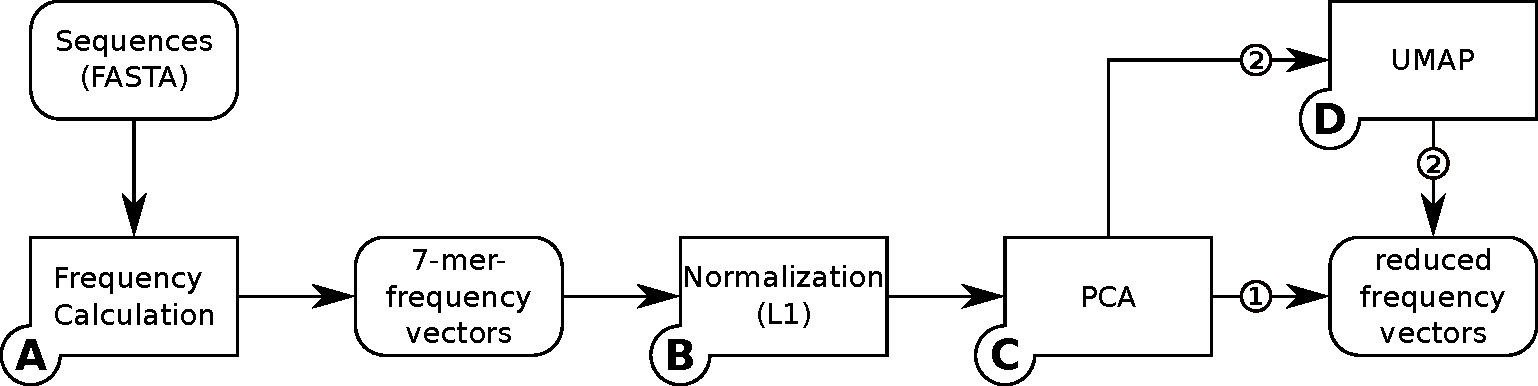
\includegraphics[width=\textwidth]{Graphics/Vectorization.pdf}
    \caption[Preprocessing pipeline]{\textbf{Preprocessing pipeline.} To create high-quality vectors representing the sequences, the FASTA file was translated to normalized vectors containing the 7-mer frequencies of the specific sequences (\textsf{\textbf{A}} and \textsf{\textbf{B}}). By workflow \textsf{\textbf{1}}, a low complexity representation of the vectors is obtained for clustering only using \texttt{PCA} (\textsf{\textbf{C}}). workflow \textsf{\textbf{2}} describes additional execution of \texttt{UMAP} that can be used after \texttt{PCA} as intermediate instead of final step (\textsf{\textbf{D}}). Reduction with workflow \textsf{\textbf{1}} or \textsf{\textbf{2}} results in reduced frequency vectors with 30 components.} 
    \label{fig:Vectorization_Pipeline}
\end{figure}

\begin{figure}[!hbt]
    \centering
    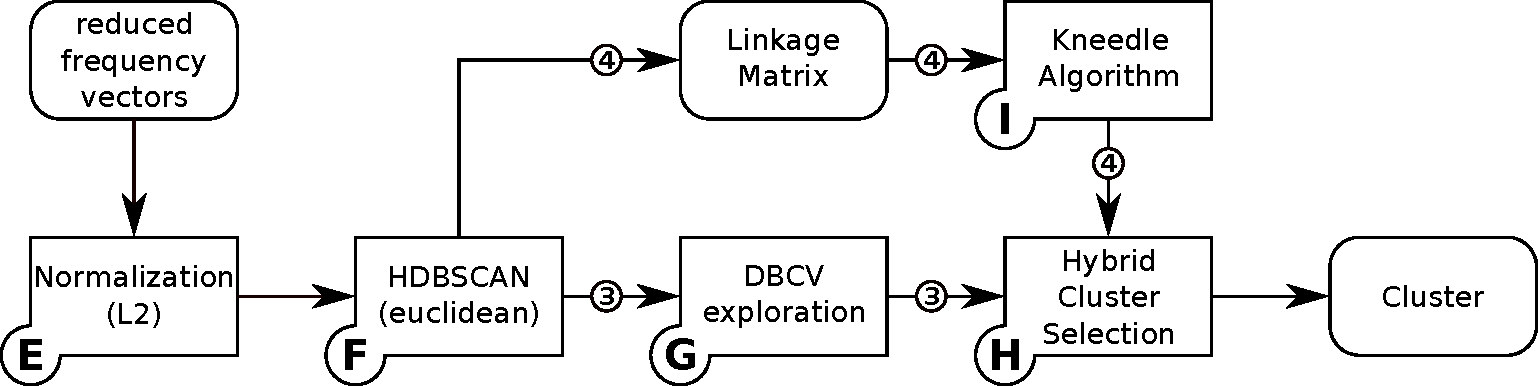
\includegraphics[width=\textwidth]{Graphics/Clustering.pdf}
    \caption[Clustering pipeline]{\textbf{Clustering pipeline.} Following the preprocessing pipeline (\autoref{fig:Vectorization_Pipeline}) normalization is used again with L2-norm as preparation for \texttt{HDBSCAN} (\textsf{\textbf{E}}). Initial \texttt{HDBSCAN} clustering (\textsf{\textbf{F}}) is performed in preparation to the $\varepsilon$ exploration using either workflow \textsf{\textbf{3}} or \textsf{\textbf{4}}. Final hybrid clustering (\textsf{\textbf{H}}) is then executed on the results of the $\varepsilon$ exploration using the Kneedle Algorithm (\textsf{\textbf{I}} and workflow \textsf{\textbf{4}} or DBCV (workflow \textsf{\textbf{3}} and \textsf{\textbf{G}}).}
    \label{fig:Clustering_Pipeline}
\end{figure}

\vspace{1em}

The method is based on the one proposed by \textcite{viehweger_addressing_2019}. Instead of using the tool \texttt{nanotext} as proposed in \textcite{viehweger_encoding_2019}, a simple 7-mer frequency calculation was implemented and used as described in \autoref{sec:Frequency}. Similar to \textcite{viehweger_addressing_2019}, the calculated vectors were clustered using the same tool \texttt{HDBSCAN} but with settings described in the \autoref{sec:HDBSCAN} instead. Since \texttt{nanotext} was not used in this project, different types of dimension reduction were performed and compared, as described in \autoref{sec:PCA} and discussed in \autoref{sec:Clustering}. With reference to the use of cosine similarity $s_{\text{cos}}(\mathbf{x}, \mathbf{y})$ as measurement for genomic similarity in \texttt{nanotext}, the use of the complementary cosine distance $d_{\text{cos}}(\mathbf{x}, \mathbf{y})$ in \texttt{HDBSCAN} was targeted (\autoref{eq:cos}) \autocite{viehweger_encoding_2019}. %To my best knowledge there is no other publication to the present day that used the same method proposed or created similar results.

\begin{equation}\label{eq:cos}
    \begin{aligned}
        d_{\text{cos}}(\mathbf{x}, \mathbf{y}) = 1 - s_{\text{cos}}(\mathbf{x}, \mathbf{y})
    \end{aligned}
\end{equation}

\begin{figure}[!hbt]
    \centering
    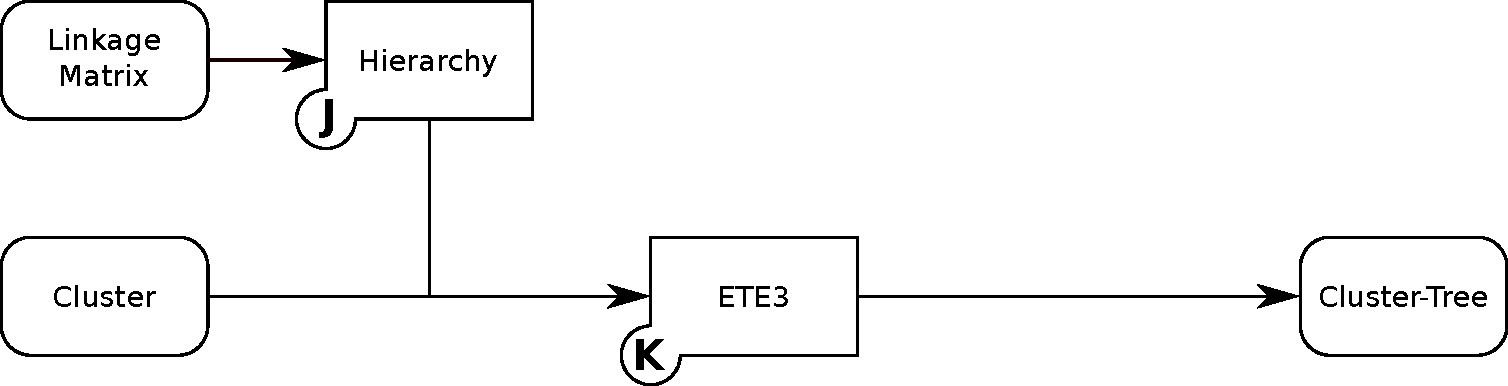
\includegraphics[width=\textwidth]{Graphics/Tree.pdf}
    \caption[Postprocessing pipeline]{\textbf{Postprocessing pipeline.} Following the clustering pipeline (\autoref{fig:Clustering_Pipeline}) the cluster-tree is build by \texttt{BioPython} and visualized by \texttt{ETE3} (\textsf{\textbf{J}}). For every cluster the vectors with the smallest distance to the other cluster members are calculated and determined as the clusters centroids (\textsf{\textbf{K}}).}
    \label{fig:Tree_Pipeline}
\end{figure}

\section{7-mer frequency calculation} \label{sec:Frequency}

The FASTA file containing the genomes of \gls{IAV} for clustering, was converted to vectors to enable clustering in high dimension by counting their 7-mer frequency (\autoref{fig:Vectorization_Pipeline} \textsf{\textbf{A}}) \autocite{edgar_muscle_2004}. $4^7$ possible constellations of the nucleotides A,C,G and T with length seven exist. Therefore, taking every constellation into consideration, the vector of every sequence has $4^7$ components. The numbers in the vector components are the number of occurrences of the related 7-mer in the sequence. The first constellation of the $4^7$ possible ones with length length is AAAAAAA, given a example sequence of the FASTA contains this 7-mer ten times, the first component of the sequences vector would be ten. \autoref{fig:k-mer} illustrates the calculation with 3-mers instead of 7-mers.

\begin{figure}[!hbt]
    \centering
    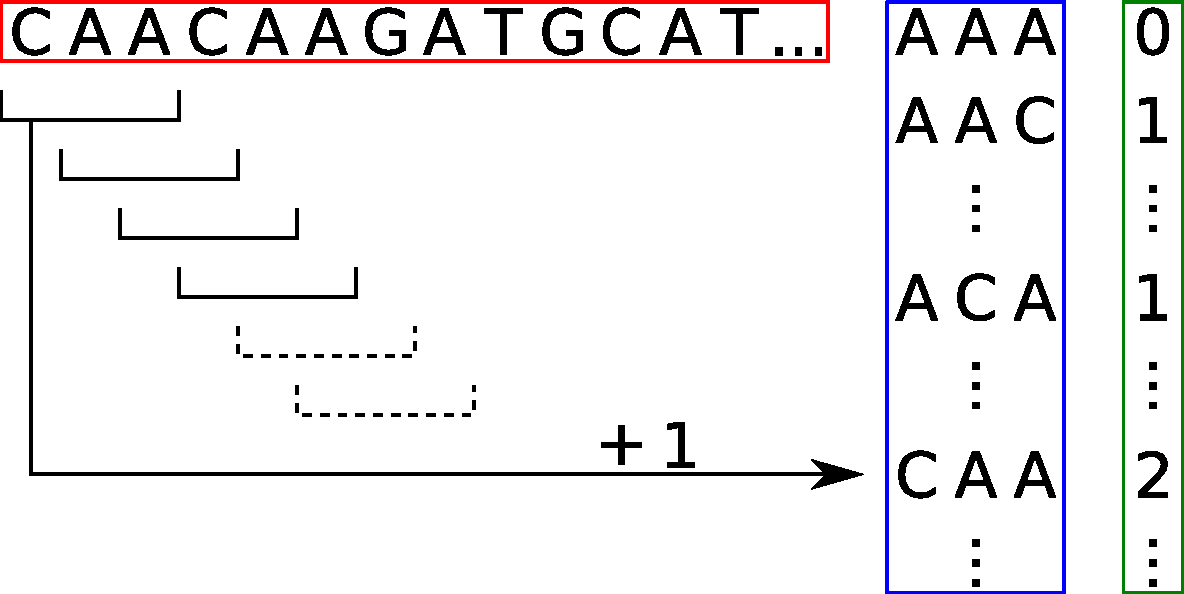
\includegraphics[width=0.5\textwidth]{Graphics/Kmer.pdf}
    \caption[$k$-mer vector creation]{\textbf{$\bm{k}$-mer vector creation.} An example genomic sequence (red box) is splitted into 3-mers. The sequences 3-mers are then compared to the list of all $4^3$ possible 3-mer constellations (blue box) Based on the occurrence number of the lists 3-mers in the sequence a vector with $4^3$ components is created (green box).}
    \label{fig:k-mer}
\end{figure}

To gain the frequency of the 7-mers all the vectors were normalized to a vector sum of one, according to L1-norm (\autoref{eq:norm1} and \autoref{fig:Vectorization_Pipeline} \textsf{\textbf{B}}). 

\begin{equation}\label{eq:norm1}
    \begin{aligned}
        \mathbf{\hat{x}} = \frac{\mathbf{x}}{\Vert\mathbf{x}\Vert_1}
    \end{aligned}
\end{equation}

\section{Dimension reduction} \label{sec:PCA}

\texttt{PCA} was used to handle the complexity of the vectors by simplification with the least loss of information possible (\autoref{fig:Vectorization_Pipeline} \textsf{\textbf{C}}) \autocite{pearson_liii_1901} \autocite{pedregosa_scikit-learn_2011}.

\vspace{1em}

Without posterior use of \texttt{UMAP} 30 components were extracted by the \texttt{PCA} (\autoref{fig:Vectorization_Pipeline} workflow \textsf{\textbf{1}}) and otherwise 100 (\autoref{fig:Vectorization_Pipeline} workflow \textsf{\textbf{2}}). Extraction of 30 or 100 components out of $4^7$ in total equals $\approx 0.18\%$ or $\approx 0.61\%$. The size limit of the \texttt{PCA} function for calculation with default setting \texttt{svd\_solver='auto'} is 500 different vectors with 500 components and at least 80\% of the components to extract. Since every maximum for standard settings was exceeded, \texttt{svd\_solver='randomized'} setting was used automatically. %\autocite{pedregosa_scikit-learn_2011}. %Randomized truncated \gls{SVD} is performed in the PCA as described in \textcite{halko_finding_2010}.

\vspace{1em}

\texttt{UMAP} was used for dimension reduction similar to \texttt{PCA}, aiming to better preserve the global structure of the data (\autoref{fig:Vectorization_Pipeline} \textsf{\textbf{D}} and workflow \textsf{\textbf{2}}) \autocite{mcinnes_umap_2020}. It is similar to the well-known \texttt{t-SNE} with better run time performance and better structure preservation in the lower dimension and less restrictions \autocite{maaten_visualizing_2008, mcinnes_umap_2020}. %Embedding is, hereby, the presentation of the used dataset in the lower dimension.
The used parameters of \texttt{UMAP} match most of the ones listed in the manual under section \glqq UMAP enhanced clustering\grqq{}\footnote{\url{https://umap-learn.readthedocs.io/en/latest/clustering.html} (accessed 07/01/2021)}. The settings are proposed to be used with \texttt{UMAP} prior to \texttt{HDBSCAN} clustering. Since the goal was clustering, not plotting 30 components was used instead of the proposed two. The neighbors number was also changed. It is recommended to be set in a range of one to 100. Based on the high number of sequences used e.~g.~, 56617 for segment 4, the highest recommended setting of 100 was used to better preserve the global picture of the data. Also based on the input size \texttt{n\_epochs=200} setting was used automatically.

\vspace{1em}

\texttt{UMAP} was used posterior to dimension reduction with \texttt{PCA}, because of the similarity to \texttt{t-SNE}. As explained in the manual of \texttt{t-SNE}\footnote{\url{https://scikit-learn.org/stable/modules/generated/sklearn.manifold.TSNE.html} (accessed 07/01/2021)}, the dimension should be reduced to a reasonable amount prior to execution to reduce noise. In section \glqq What is the difference between PCA / UMAP / VAEs?\grqq{} of the \texttt{UMAP} manual\footnote{\url{https://umap-learn.readthedocs.io/en/latest/faq.html} (accessed 07/01/2021)} a pipeline is proposed, to reduce from high dimension with \texttt{PCA}, continue with reduction by \texttt{UMAP} and cluster with \texttt{HDBSCAN} and is, therefore, used as reference. Reduction with \texttt{UMAP} to 30 components posterior to \texttt{PCA} with 100 components also provided a comfortable balancing of computational effort of both methods, while preserving $\approx 85\%$ explained variance with \texttt{PCA} \autocite{mcinnes_umap_2020}. 

\section{Hybrid clustering} \label{sec:HDBSCAN}

\texttt{HDBSCAN} was used to cluster the reduced vectors. It is an clustering algorithm proposed by \textcite{campello_hierarchical_2015} as a novel version of the well-known \texttt{DBSCAN} \autocite{hutchison_density-based_2013}. Execution of \texttt{HDBSCAN} involves varying values of $\varepsilon$, thus, not one specific threshold is used to define the clusters, but instead clusters of varying densities are extracted based on their stability \autocite{mcinnes_hdbscan_2017}. \texttt{HDBSCAN} was used with hybrid clustering setting as proposed in \textcite{malzer_hybrid_2020}, combining \texttt{HDBSCAN} it with \texttt{DBSCAN}. Thereby, some of the disadvantages of using either of these methods can be avoided \autocite{mcinnes_hdbscan_2017, moulavi_density-based_2014}. Since \texttt{DBSCAN} is a hierarchical clustering tool, it is dependent on a strict threshold $\varepsilon$ for clustering. Vectors not surrounded by $k$ other vectors in a radius defined by this threshold value $\varepsilon$ are omitted as single vector clusters or noise \autocite{ester_density-based_1996, schubert_dbscan_2017}. Standard \texttt{HDBSCAN}, on the other hand, tend to create unwanted micro-clusters in areas of high density \autocite{mcinnes_hdbscan_2017}. Using the hybrid \texttt{HDBSCAN} proposed in \autocite{malzer_hybrid_2020}, a threshold value $\varepsilon$ can be used to extract these high density areas as single clusters with \texttt{DBSCAN}, but still use the standard \texttt{HDBSCAN} for the otherwise omitted vectors (\autoref{fig:Hybrid} and \autoref{fig:Clustering_Pipeline} \textsf{\textbf{H}}). Hybrid \texttt{HDBSCAN} is, thus, clustering with \texttt{DBSCAN},resulting in a \textbf{raw} cluster number containing finished clusters and omitted single vector clusters, and subsequent standard \texttt{HDBSCAN}, reducing the \textbf{final} cluster number by clustering the omitted vectors.

\vspace{1em}

This method is useful when having a small cluster size value, while still aiming to cluster high-density areas together exactly suitable for the proposed clustering. Specific strains of \gls{IAV} are sequenced a lot more, thereby probably creating high-density areas that should be clustered together with \texttt{DBSCAN}. The small cluster size is, thereby, used to find small clusters of rare sequenced variants by \texttt{HDBSCAN}, with possibly important mutations in low-density areas \autocite{malzer_hybrid_2020}. As explained, the smallest minimum cluster size of two was used to capture, in the best case, even genomes with rare appearing mutations, in their own clusters. To declare as least vectors as possible as noise, the minimum samples value $k$ was also set to the minimum one. Standard \texttt{HDBSCAN} was once performed without the hybrid setting, in preparation of $\varepsilon$ exploration as described in \autoref{sec:epsilon} \autoref{fig:Clustering_Pipeline} \textsf{\textbf{F}}). Hybrid \texttt{HDBSCAN} clustering was used with the same settings plus respective $\varepsilon$ value \autoref{fig:Clustering_Pipeline} \textsf{\textbf{H}}).

\vspace{1em}

Distance calculations by \texttt{HDBSCAN} were performed with the euclidean distance setting due to an open issue in the GitHub Repository of \texttt{HDBSCAN}\footnote{\url{https://github.com/scikit-learn-contrib/hdbscan/issues/69} (accessed 06/02/21)}. In the issue the inability to use cosine distance metric with \texttt{HDBSCAN} and the approximation of it by chord distance metric, is described. Given that chord distance metric is also not available firsthand, the possibility to use normalization of the vectors with L2-norm, prior to clustering with euclidean metric setting is also mentioned \autoref{fig:Clustering_Pipeline} \textsf{\textbf{E}}). 

\begin{figure}[!hbt]
    \centering
    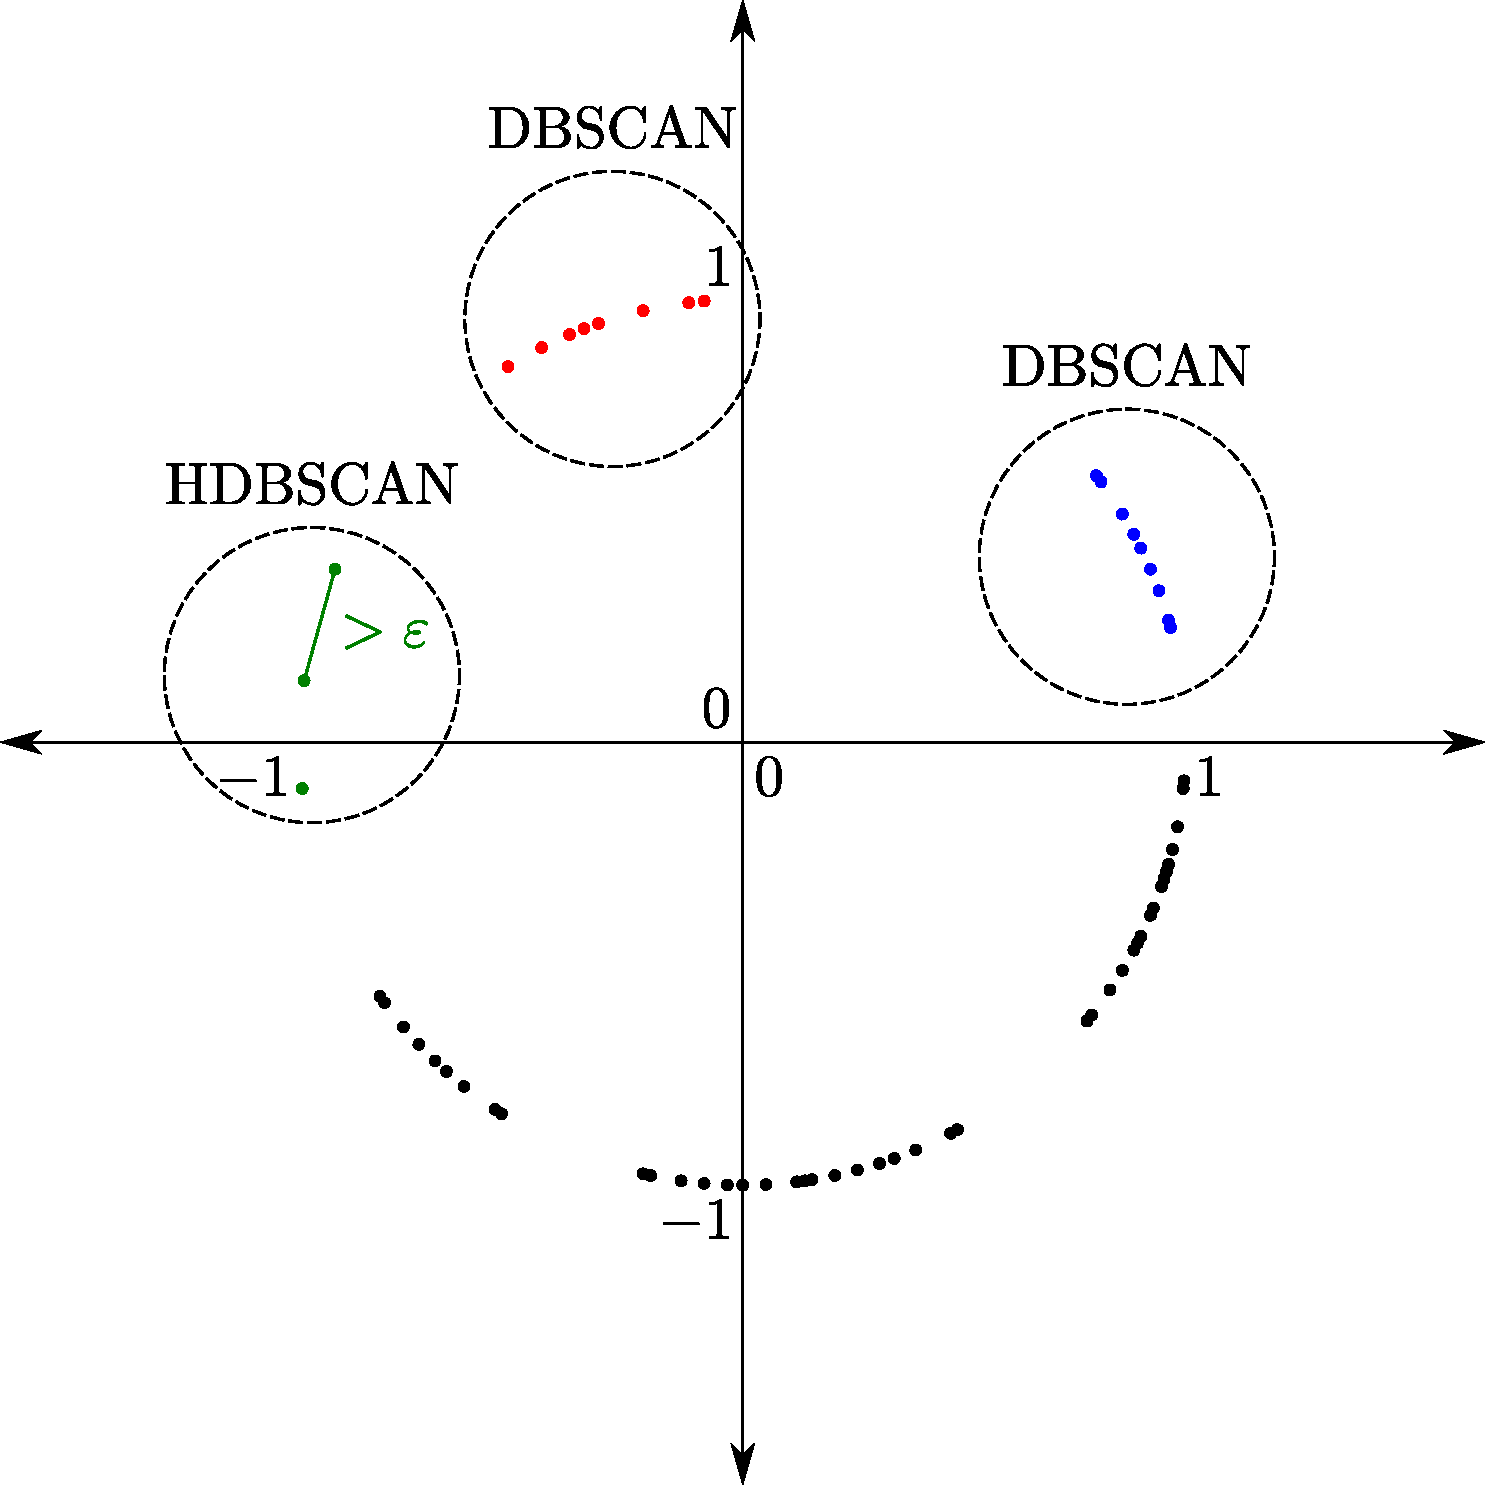
\includegraphics[width=\textwidth]{Graphics/Hybrid.pdf}
    \caption[Hybrid clustering threshold]{\textbf{Hybrid clustering threshold.} The hybrid clustering \texttt{HDBSCAN} differentiate between clusters where vectors are connected by distances smaller and higher than $\varepsilon$. When the distance is smaller, the \texttt{DBSCAN} algorithm is used and clusters are generated based on this threshold value $\varepsilon$ by combining vectors with smaller distance. Omitted vectors, not having a given number of $k=1$ vectors in reachable distance of $\varepsilon$ and are, therefore, impossible to be clustered by \texttt{DBSCAN} are subsequently clustered with \texttt{HDBSCAN} building clusters with higher threshold if appropriate. The graphic is based on \glqq Combining HDBSCAN* with DBSCAN\grqq{} in the manual\footnotemark and adapted to the calculations in this project, as a two dimensional example.}
    \label{fig:Hybrid}
\end{figure}

\begin{figure}[!hbt]
    \centering
    \begin{subfigure}[b]{0.475\textwidth}
        \caption[Chord]{\textbf{Chord distance}}
        \label{subfig:Chord}
        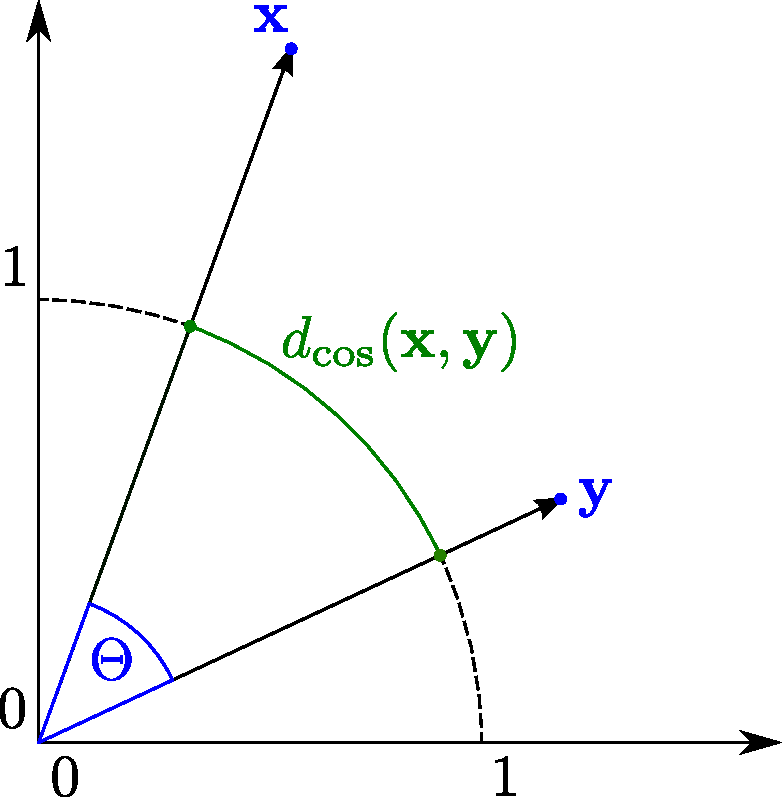
\includegraphics[width=\textwidth]{Graphics/Chord.pdf}
    \end{subfigure}
    \hfill
    \begin{subfigure}[b]{0.475\textwidth}
        \caption[L2]{\textbf{L2-norm normalized euclidean distance}}
        \label{subfig:L2}            
        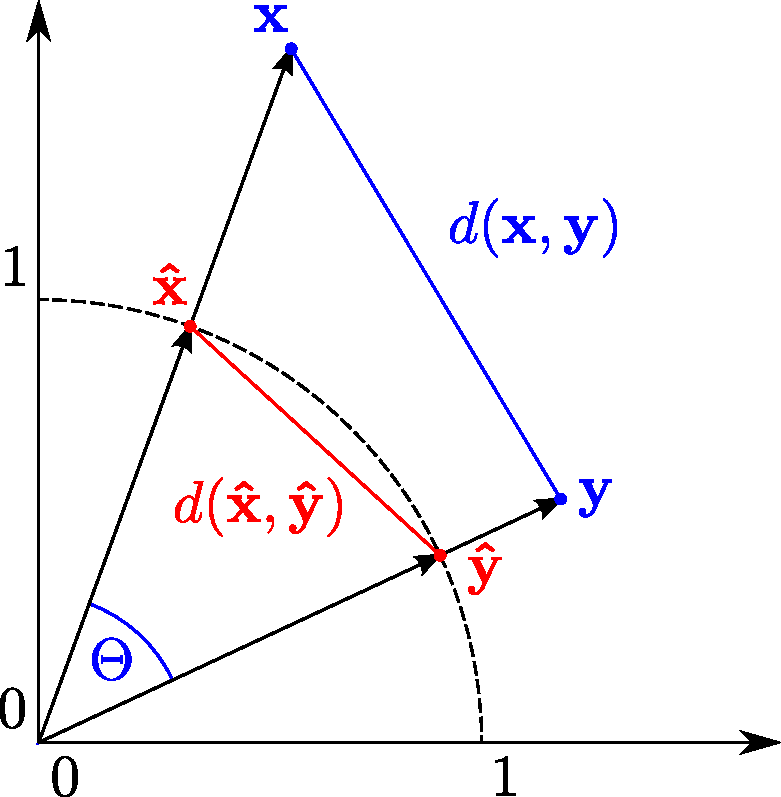
\includegraphics[width=\textwidth]{Graphics/L2.pdf}
    \end{subfigure}
    \caption[Chord calculation background]{\textbf{Chord calculation background.} The chord can be calculated with the radius similar for both vectors and the information of the angle of two vectors to the origin of the coordinate system. Since this information is not always available or sometimes expensive to calculate for a high number of vectors, the euclidean distance can be used with a L2-norm of both vectors equal to $r$ for similar results instead. To approximate cosine distance, the same calculation of euclidean distance is used with L2-norm equal to $r = 1$. To always obtain similar values of L2-norm equal to one, L2-norm normalization is used on every vector.}
    \label{fig:L2_Normalisation_Background}
\end{figure}

\begin{equation}\label{eq:norm2}
    \begin{aligned}
        \mathbf{\hat{x}} = \frac{\mathbf{x}}{\Vert\mathbf{x}\Vert_2}
    \end{aligned}
\end{equation}

Calculation of chord distance $d_{\text{chord}}$ is possible when having two vectors, here as an example named as $\mathbf{a}$ and $\mathbf{b}$ with the same L2-norm equal to a radius $r$ of a sphere centered to the origin of the coordinate system and an angle of $\Theta$ (\autoref{eq:chord1} and \autoref{subfig:Chord}) \autocite{maor_trigonometric_2013}. The euclidean distance $d_{\text{eucl}}$ is equal to the chord distance for the same vectors.
\footnotetext{\url{https://hdbscan.readthedocs.io/en/latest/how_to_use_epsilon.html} (accessed 07/01/2021)}

\begin{equation}\label{eq:chord1}
    \Vert\mathbf{a}\Vert_2 = \Vert\mathbf{b}\Vert_2 = r \Rightarrow 
    \begin{aligned}
        d_{\text{chord}}(\mathbf{a},\mathbf{b}) &= 2 \cdot r \sin \left(\frac{\Theta}{2}\right)\\
        &= d_{\text{eucl}}(\mathbf{a},\mathbf{b})
    \end{aligned}
\end{equation}

Thus, in this project, chord distance can be calculated with the euclidean distance metric, posterior to the normalization with the L2-norm, which scales the vectors to the unit sphere \autoref{subfig:L2}. 

\begin{equation}\label{eq:chord2}
    \Vert\mathbf{\hat{x}}\Vert_2 = \Vert\mathbf{\hat{y}}\Vert_2 = 1 \Rightarrow 
    \begin{aligned}
        d_{\text{chord}}(\mathbf{\hat{x}},\mathbf{\hat{y}}) &= d_{\text{eucl}}(\mathbf{\hat{x}},\mathbf{\hat{y}})\\
        &= \Vert\mathbf{\hat{x}} - \mathbf{\hat{y}}\Vert_2
    \end{aligned}
\end{equation}

The calculation of the chord distance, by L2-norm normalized vectors euclidean distance, is, thereby, integrated into the mutual reachability distance calculation of \texttt{HDBSCAN}. The mutual reachability distance is the maximum of the chord distance and the core distances of two vectors (\autoref{eq:reach}). The core distance is the minimum radius necessary to include five other vectors around a given vector \autocite{mcinnes_hdbscan_2017}. Threshold $\varepsilon$ is used on the mutual reachability distances between the vectors \autoref{fig:Hybrid}. 

\begin{equation}\label{eq:reach}
    \begin{aligned}
        d_{\text{mreach}-k}(\mathbf{\hat{x}},\mathbf{\hat{y}}) &= \max \{ \text{core}_k(\mathbf{\hat{x}}), \text{core}_k(\mathbf{\hat{y}}), d_{\text{eucl}}(\mathbf{\hat{x}},\mathbf{\hat{y}}) \}
    \end{aligned}
\end{equation}

The used chord distance is proportional with the initially intended to use cosine distance as shown in \autoref{eq:chord3}. Dividing the squared chord distance by two results in the cosine distance of the vectors \autoref{fig:Normalisation_Methods}.

\begin{equation}\label{eq:chord3}
    \Vert\mathbf{\hat{x}}\Vert_2 = \Vert\mathbf{\hat{y}}\Vert_2 = 1 \Rightarrow 
    \begin{aligned}  
        d_{\text{chord}}(\mathbf{\hat{x}},\mathbf{\hat{y}})^2 &= \Vert\mathbf{\hat{x}} - \mathbf{\hat{y}}\Vert_2^2\\
        &= (\mathbf{\hat{x}} - \mathbf{\hat{y}})^\top (\mathbf{\hat{x}} - \mathbf{\hat{y}})\\
        &= \mathbf{\hat{x}}^\top \mathbf{\hat{x}} - 2 \mathbf{\hat{x}}^\top \mathbf{\hat{y}} + \mathbf{\hat{y}}^\top \mathbf{\hat{y}}\\
        &= 2 - 2\mathbf{\hat{x}}^\top \mathbf{\hat{y}}\\
        &= 2 - 2 \cos(\Theta)\\
        &= 2 \cdot (1 - \cos(\Theta))\\
        &= 2 \cdot d_{\text{cos}}(\mathbf{\hat{x}},\mathbf{\hat{y}})
    \end{aligned}
\end{equation}

\begin{figure}[!hbt]
    \centering
    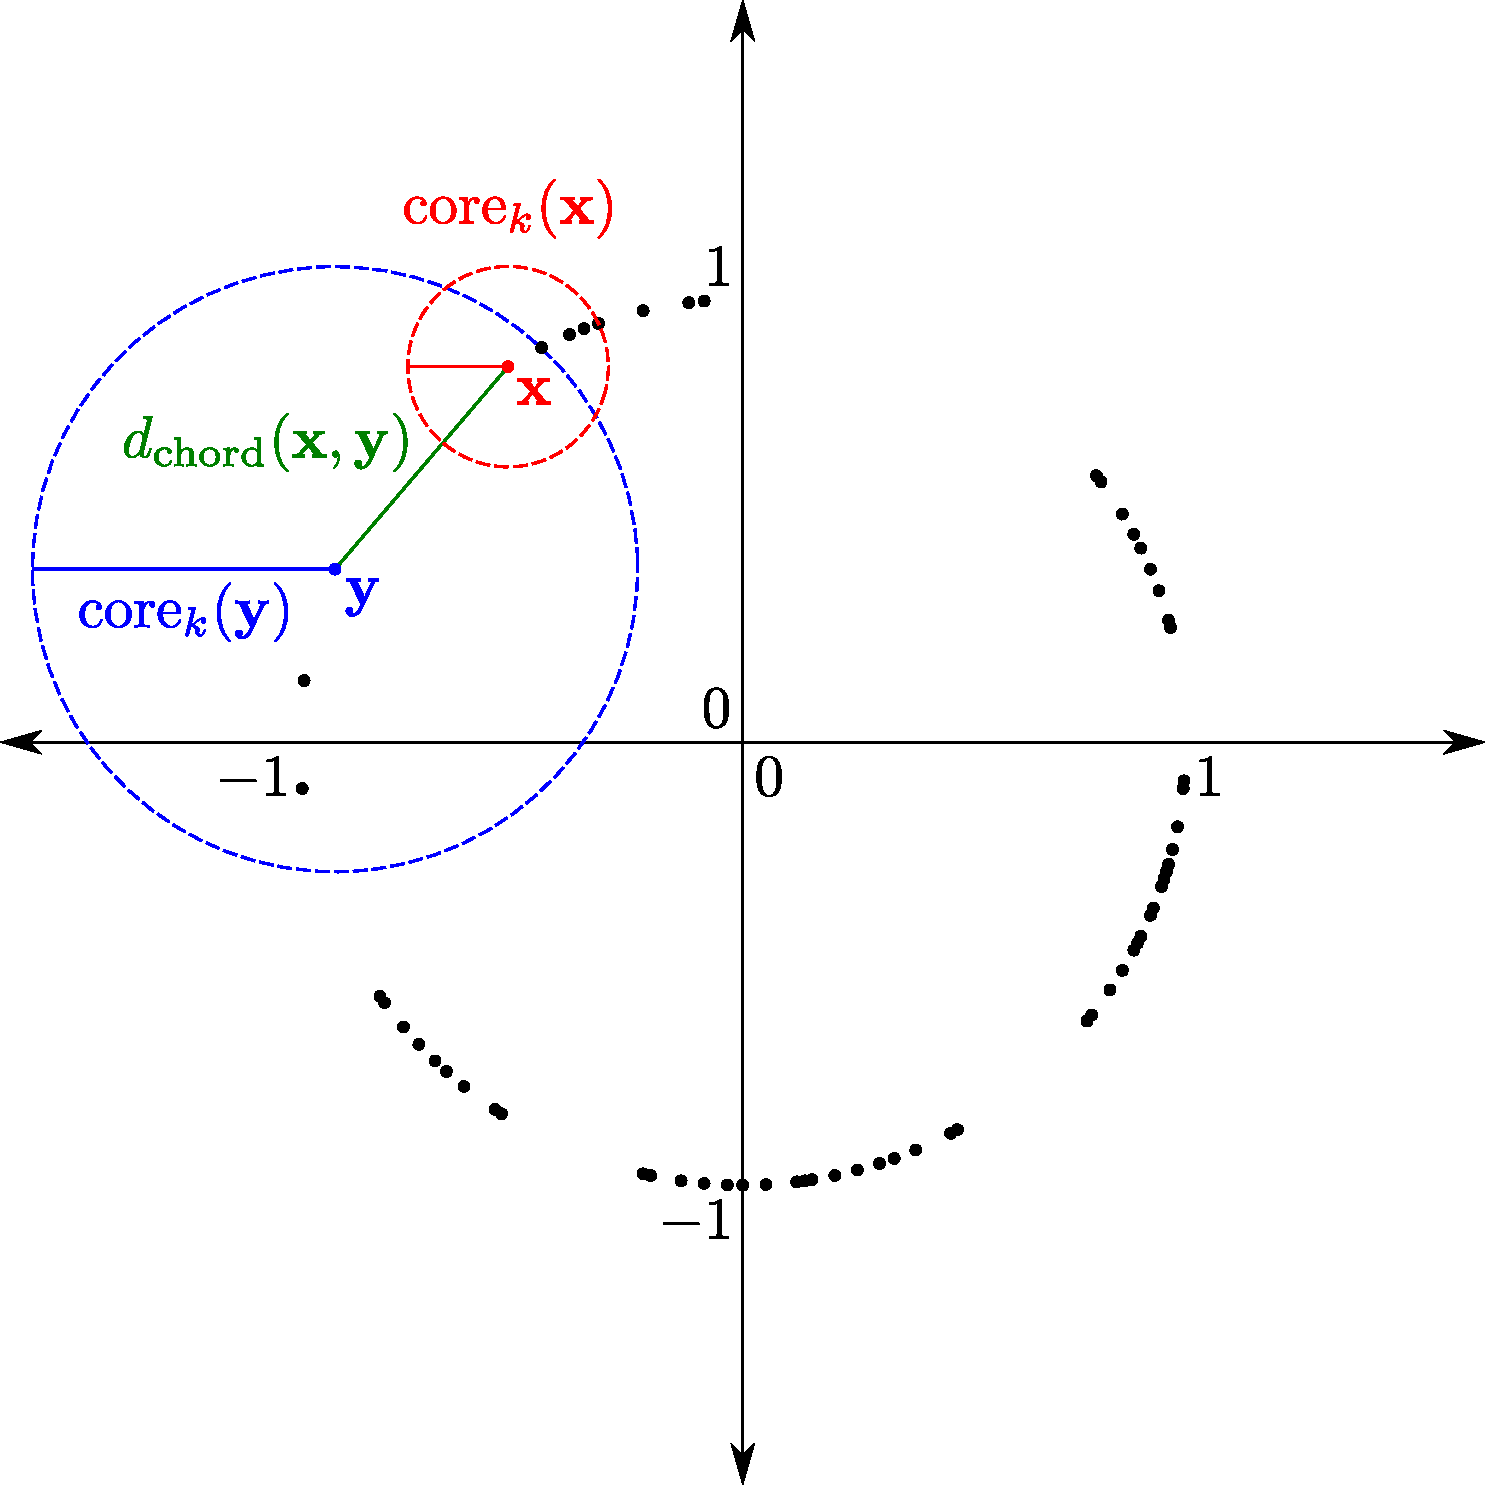
\includegraphics[width=\textwidth]{Graphics/HDB.pdf}
    \caption[Mutual reachability calculation]{\textbf{Mutual reachability calculation.} A low dimension representation of the calculation \texttt{HDBSCAN} performed in this project. To calculate the mutual reachability distance, the smallest radius is calculated to include exactly $k = 1$ vectors. This example should demostrate the calculation for two L2-norm normalized vectors $\mathbf{\hat{x}}$ in blue and $\mathbf{\hat{y}}$ in red, with the value of one for $k$ used in the project. The euclidean distance between these vectors is then calculated and compared to the radii. The maximum of both radii and the euclidean distance is the mutual reachability distance (\autoref{eq:reach}). The used parameters make the mutual reachability distance always be the euclidean distance since the radius with $k=1$ other vectors can only reach the euclidean distance at maximum.}
    \label{fig:HDB}
\end{figure}

\section{Epsilon selection} \label{sec:epsilon}

To find an appropriate value for $\varepsilon$, two different methods were used and compared (\autoref{fig:Clustering_Pipeline} workflow \textsf{\textbf{3}} and \textsf{\textbf{4}}). The first method, the \gls{DBCV} exploration in \autoref{fig:Clustering_Pipeline} \textsf{\textbf{G}}, is based on repeated execution of hybrid \texttt{HDBSCAN} with different settings for $\varepsilon$ and comparison by the \gls{DBCV}. The \gls{DBCV} is a calculation based on the minimum spanning tree to estimate overall cluster density \autocite{moulavi_density-based_2014}. To enable the calculation hybrid \texttt{HDBSCAN} was performed with \texttt{gen\_min\_span\_tree=True} setting.

\vspace{1em}

Second method for $\varepsilon$ exploration was performed using the Kneedle Algorithm on the linkage matrix created by the initially performed of standard \texttt{HDBSCAN} clustering (\autoref{fig:Clustering_Pipeline} \textsf{\textbf{F}} and \textsf{\textbf{I}}) \autocite{satopaa_finding_2011}. With increasing cluster number, the distance threshold $\varepsilon$ of hierarchical clustering decreases. This describes a decreasing curve of convex type with distance threshold on the y- and cluster number on the x-axis. The knee is the number of clusters at the point in the polynomial representation of the curve with maximal acceleration. Polynomial representation was used to find the maximum acceleration of the smoothed curve. Therefore the settings \texttt{curve='concave'}, \texttt{direction='increasing'} and \texttt{interp\_method='interp1d'} were used to find the optimal number of clusters. The optimal number of clusters was converted to the respective $\varepsilon$ threshold.

\vspace{1em}

Knee point selection was restricted to a given area between one and a maximum value of 500. The maximum was chosen to include the area with the highest expected differences. The best Knee point was expected to be less than 100, a higher value was used to prevent forcing the number of clusters to be maximal 100. 

\section{Alignments and vector calculations} \label{sec:MAFFT}

The labeled cluster trees were created by \texttt{ETE3} with a newick file, generated according to a feature request, proposed for the \texttt{SciPy}\footnote{\url{https://github.com/scipy/scipy/issues/8274} (accessed 06/02/21)} (\autoref{fig:Tree_Pipeline} \textsf{\textbf{J}}) \autocite{huerta-cepas_ete_2016}. Clusters centroid vectors were selected by calculating euclidean distance between all the vectors of a cluster to each other. The vector with the smallest mean distance was declared as centroid (\autoref{fig:Tree_Pipeline} \textsf{\textbf{K}}). 

%The materials described in the following were only used for the centroid guide tree creation and the analyses on H13/H16 sequences in the \autoref{sec:Clustering_Anomalies} to \autoref{sec:Dimension_Reduction} and are, therefore, not included in the novel \gls{IAV} clustering tool (\autoref{fig:Alignment_Pipeline} and \autoref{fig:Precalc_Pipeline}).

\begin{figure}[!hbt]
    \centering
    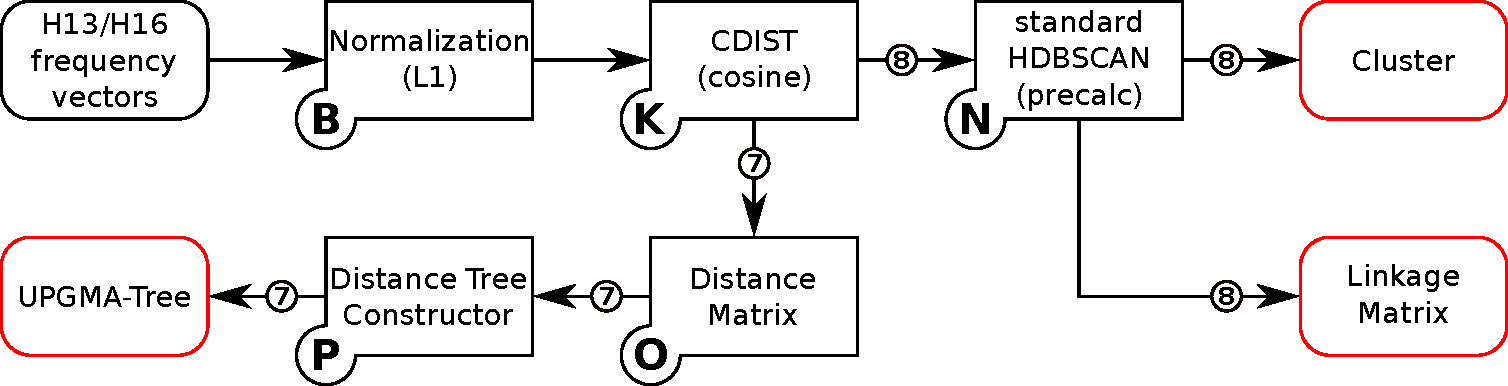
\includegraphics[width=\textwidth]{Graphics/Precalculated.pdf}
    \caption[Precalculation pipeline]{\textbf{Precalculation pipeline.} For the precalculated trees the L1-normalized 7-mer frequency vectors distances were calculated and used for clustering by \texttt{HDBSCAN} (\textsf{\textbf{B}}, \textsf{\textbf{K}}, \textsf{\textbf{N}} and workflow \textsf{\textbf{7}}) and on the other hand processed with \texttt{BioPython} for \gls{UPGMA} tree creation and visualization by \texttt{ETE3} (\textsf{\textbf{N}} and \textsf{\textbf{8}}). Results from this pipeline were visualized according to \autoref{fig:Tree_Pipeline}.}
    \label{fig:Precalc_Pipeline}
\end{figure}

\begin{figure}[!hbt]
    \centering
    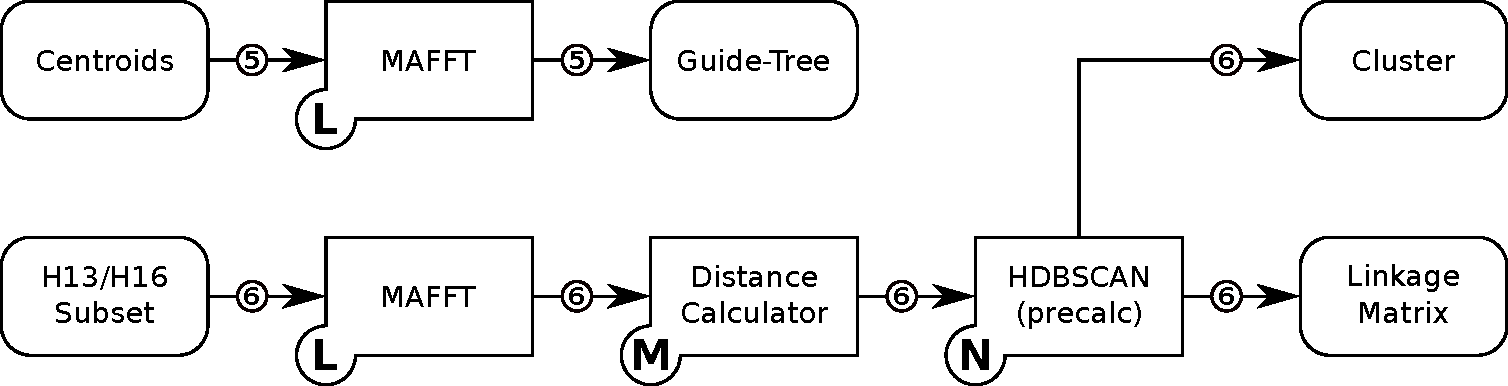
\includegraphics[width=\textwidth]{Graphics/Alignment.pdf}
    \caption[Alignment pipeline]{\textbf{Alignment pipeline.} The sequences related to the centroid vectors were aligned using \texttt{MAFFT} resulting in the output as guide-tree visualized by \texttt{ETE3} (\textsf{\textbf{L}} and workflow \textsf{\textbf{5}}). A small FASTA subset of H13/H16 was also aligned by \texttt{MAFFT} prior to evolutionary distance calculation with \texttt{BioPython} and clustering with \texttt{HDBSCAN} (\textsf{\textbf{L}}, \textsf{\textbf{M}}, \textsf{\textbf{N}} and workflow \textsf{\textbf{6}}). Results from this pipeline were visualized according to \autoref{fig:Tree_Pipeline}.}
    \label{fig:Alignment_Pipeline}
\end{figure}

\begin{figure}[!hbt]
    \centering
    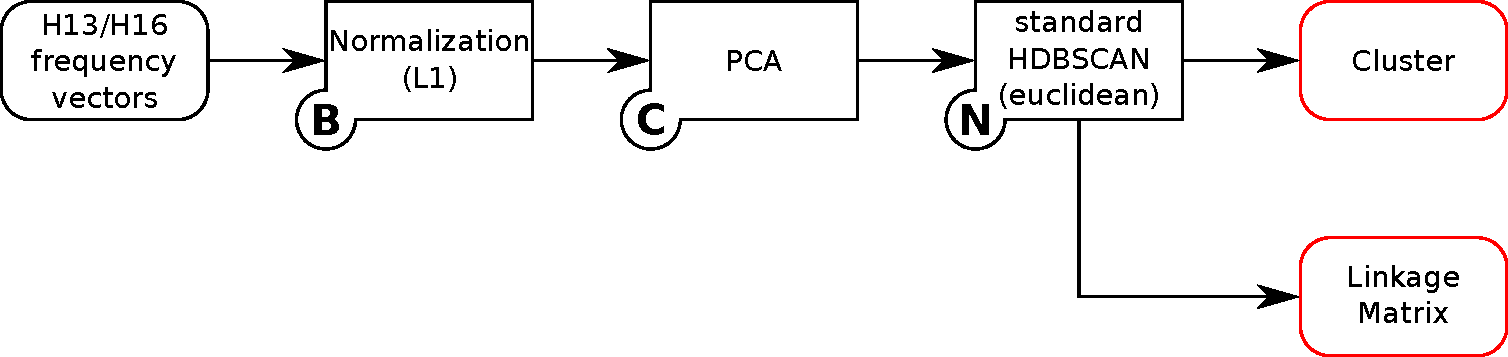
\includegraphics[width=\textwidth]{Graphics/Simple.pdf}
    \caption[Simplified clustering pipeline]{\textbf{Simplified clustering pipeline.} For the simplified clustering on the sequence subset, the the L1-normalized 7-mer vectors were reduced with \texttt{PCA} (\textsf{\textbf{B}} and \textsf{\textbf{C}}). Following the dimension reduction, the vectors were normlized again acording to L2-norm and clustered by \texttt{HDBCSCAN} (\textsf{\textbf{E}} and \textsf{\textbf{N}}). Results from this pipeline were visualized according to \autoref{fig:Tree_Pipeline}.}
    \label{fig:Simple_Pipeline}
\end{figure}

The precalculated trees were created using cosine distance calculation on the L1-norm normalized 7-mer frequency vectors of the segment 4 H13 and H16 sequences of the FASTA (\autoref{fig:Precalc_Pipeline} \textsf{\textbf{F}}). The calculated distances were used for \gls{UPGMA} tree building with \texttt{BioPython} (\autoref{fig:Alignment_Pipeline} \textsf{\textbf{O}} and \textsf{\textbf{P}}). The vectors were also clustered by \texttt{HDBSCAN} using the calculated distances with \texttt{metric='precalculated'}. Other settings were used as described in \autoref{sec:HDBSCAN} without hybrid clustering.

\vspace{1em}

\texttt{MAFFT} was used for \glspl{MSA} and guide tree creation with \texttt{treeout=True} on the centroid sequences and on the FASTA subset containing H13 and H16 sequences of segment 4 (\autoref{fig:Alignment_Pipeline} \textsf{\textbf{L}}) \autocite{katoh_mafft_2013}. The \gls{MSA} of the FASTA subset was converted to evolutionary distances with \texttt{BioPython} and clustered by \texttt{HDBSCAN} (\autoref{fig:Alignment_Pipeline} \textsf{\textbf{M}} and \textsf{\textbf{N}}). Pairwise alignments in \autoref{sec:Serotype_Classification} were performed using \texttt{BioPython}.
    
    \glsresetall
    \setcounter{table}{0}
    \setcounter{figure}{0}
    \setcounter{equation}{0}

    \chapter{Results and Discussion} \label{chap:Results_and_Discussion}

\begin{figure}[!hbt]
    \centering
    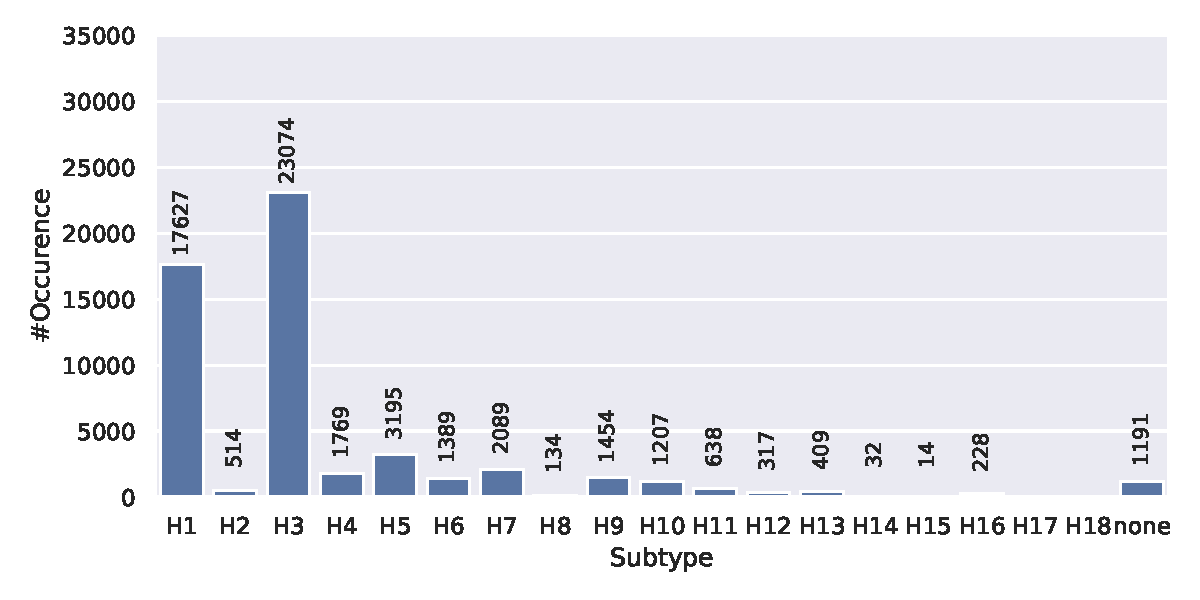
\includegraphics[width=\dimexpr\textwidth-2\fboxsep-2\fboxrule,fbox]{PCA/Data_Overview_Segment_4_H.pdf}
    \caption[Segment 4 \Acrlong{HA} Antigen Subtype Frequency]{\textbf{Segment 4 \Acrlong{HA} Antigen Subtype Frequency.} .}
    \label{fig:Frequency_4}
\end{figure}

\begin{figure}[!hbt]
    \centering
    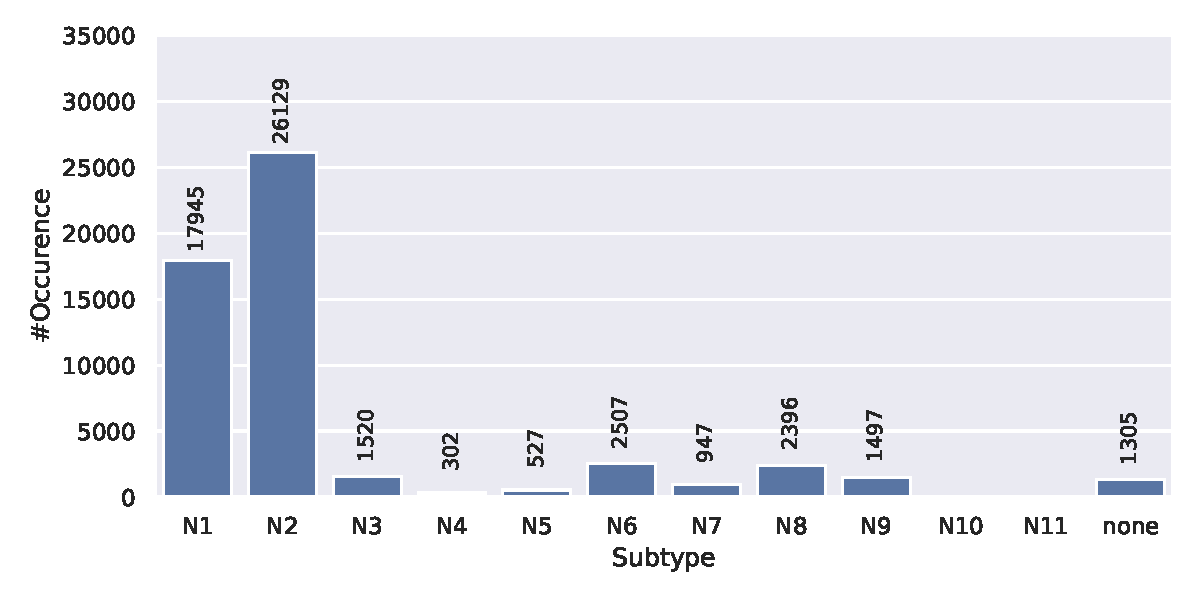
\includegraphics[width=\dimexpr\textwidth-2\fboxsep-2\fboxrule,fbox]{PCA/Data_Overview_Segment_6_N.pdf}
    \caption[Segment 6 \Acrlong{NA} Antigen Subtype Frequency]{\textbf{Segment 4 \Acrlong{NA} Antigen Subtype Frequency.} .}
    \label{fig:Frequency_6}
\end{figure}

\section{Clustering} \label{sec:3.1}

\blindtext

\begin{figure}
    \begin{adjustbox}{minipage=\dimexpr\textwidth-2\fboxsep-2\fboxrule,fbox}
        \begin{subfigure}[b]{0.475\textwidth}
            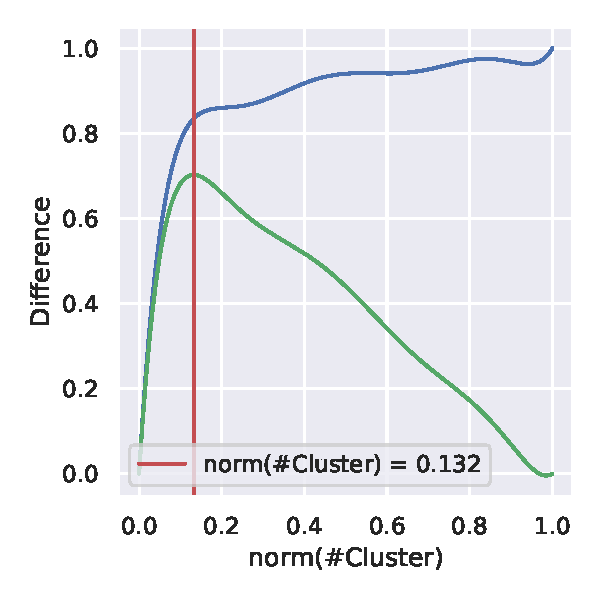
\includegraphics[width=\textwidth]{PCA/Cluster_Knee_Segment_4.pdf}
            \caption[Kneedle Algorithm]{\textbf{Kneedle Algorithm}}
            \label{fig:3.1.1a}
        \end{subfigure}
        \hfill
        \begin{subfigure}[b]{0.475\textwidth}
            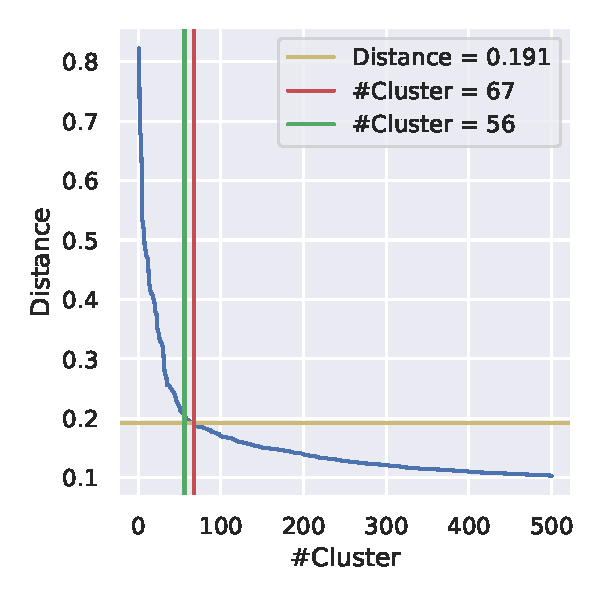
\includegraphics[width=\textwidth]{PCA/Cluster_Elbow_Knee_Segment_4.pdf}
            \caption[Kneedle Knee]{\textbf{Kneedle Knee}}
            \label{fig:3.1.1b}
        \end{subfigure}
        \vskip\baselineskip
        \begin{subfigure}[b]{0.475\textwidth}
            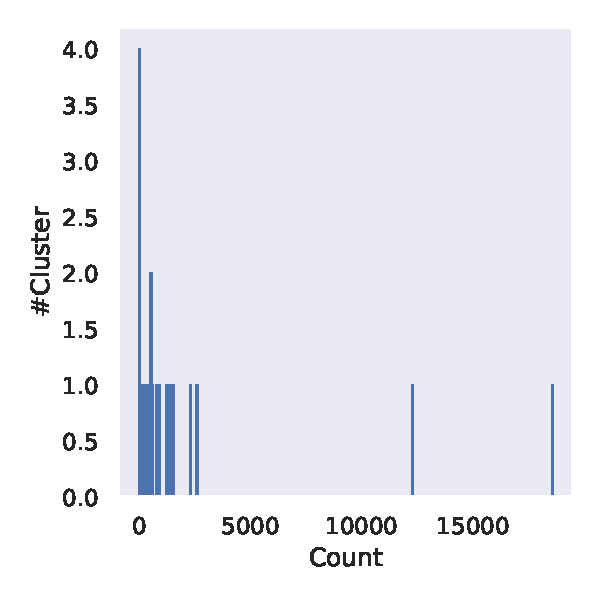
\includegraphics[width=\textwidth]{PCA/Cluster_Distribution_Segment_4.pdf}
            \caption[Cluster Distribution]{\textbf{Cluster Distribution}}
            \label{fig:3.1.1c}
        \end{subfigure}
        \hfill
        \begin{subfigure}[b]{0.475\textwidth}
            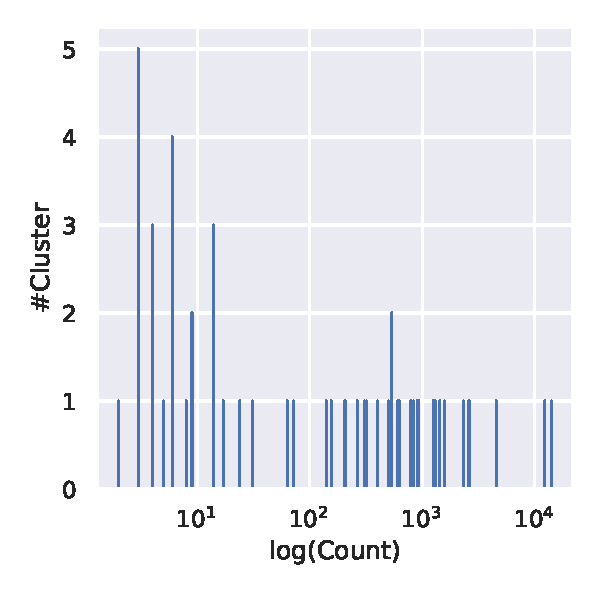
\includegraphics[width=\textwidth]{PCA/Cluster_Distribution_Log_Segment_4.pdf}
            \caption[Logarithmic Distribution]{\textbf{Logarithmic Distribution}}
            \label{fig:3.1.1d}
        \end{subfigure}
    \end{adjustbox}
    \caption[Knee based Segment 4 Clustering with PCA]{\textbf{Knee based Segment 4 Clustering with PCA.}.}
    \label{fig:3.1.1}
\end{figure}

\begin{figure}
    \begin{adjustbox}{minipage=\dimexpr\textwidth-2\fboxsep-2\fboxrule,fbox}
        \begin{subfigure}[b]{0.475\textwidth}
            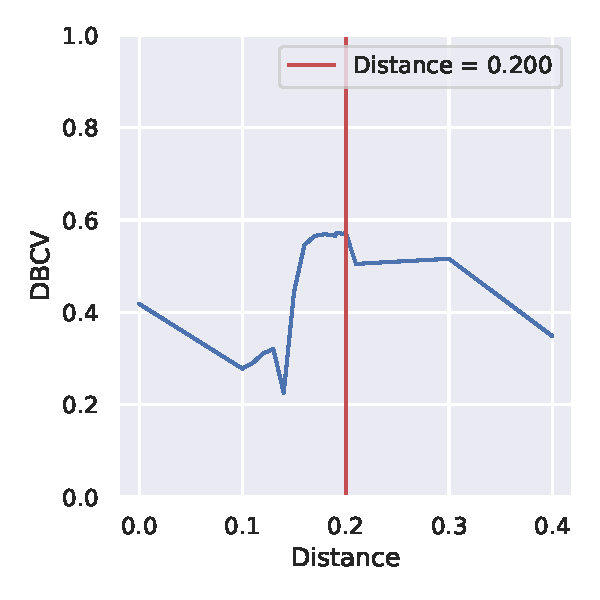
\includegraphics[width=\textwidth]{PCA/Cluster_DBCV_Segment_4.pdf}
            \caption[DBCV Exploration]{\textbf{DBCV Exploration}}
            \label{fig:3.1.2a}
        \end{subfigure}
        \hfill
        \begin{subfigure}[b]{0.475\textwidth}
            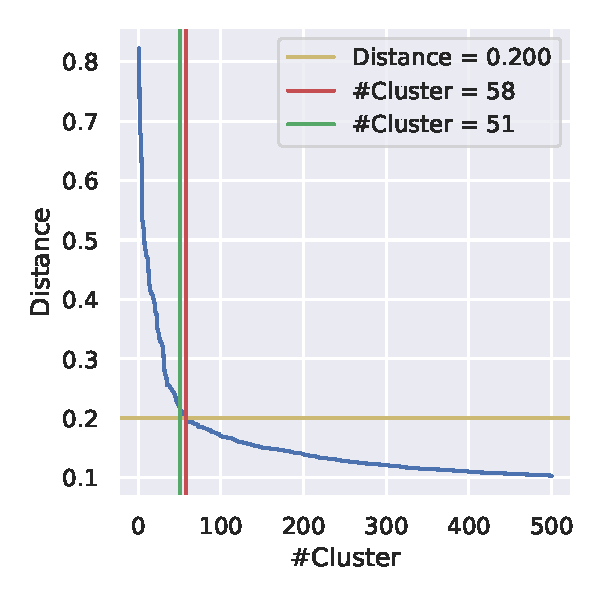
\includegraphics[width=\textwidth]{PCA/Cluster_Elbow_DBCV_Segment_4.pdf}
            \caption[DBCV Knee]{\textbf{DBCV Knee}}
            \label{fig:3.1.2b}
        \end{subfigure}
        \vskip\baselineskip
        \begin{subfigure}[b]{0.475\textwidth}
            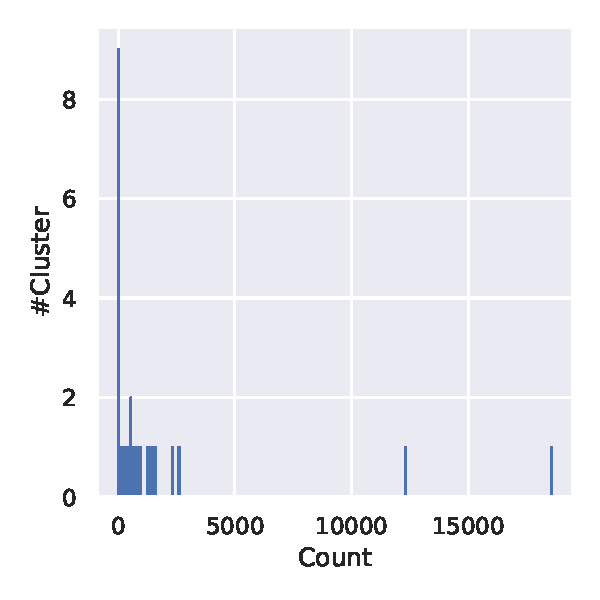
\includegraphics[width=\textwidth]{PCA/Cluster_Distribution_Segment_4_alternative.pdf}
            \caption[Cluster Distribution]{\textbf{Cluster Distribution}}
            \label{fig:3.1.2c}
        \end{subfigure}
        \hfill
        \begin{subfigure}[b]{0.475\textwidth}
            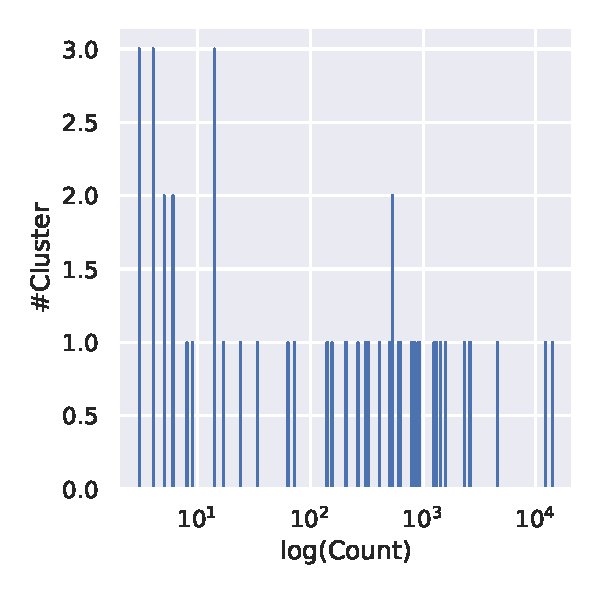
\includegraphics[width=\textwidth]{PCA/Cluster_Distribution_Log_Segment_4_alternative.pdf}
            \caption[Logarithmic Distribution]{\textbf{Logarithmic Distribution}}
            \label{fig:3.1.2d}
        \end{subfigure}
    \end{adjustbox}
    \caption[DBCV based Segment 4 Clustering with PCA]{\textbf{DBCV based Segment 4 Clustering with PCA.}.}
    \label{fig:3.1.2}
\end{figure}

\begin{figure}
    \begin{adjustbox}{minipage=\dimexpr\textwidth-2\fboxsep-2\fboxrule,fbox}
        \begin{subfigure}[b]{0.475\textwidth}
            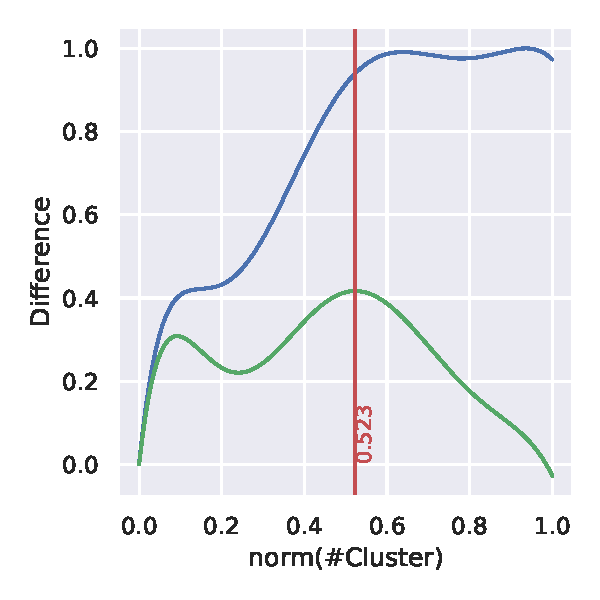
\includegraphics[width=\textwidth]{UMAP/Cluster_Knee_Segment_4.pdf}
            \caption[Kneedle Algorithm]{\textbf{Kneedle Algorithm}}
            \label{fig:3.1.3a}
        \end{subfigure}
        \hfill
        \begin{subfigure}[b]{0.475\textwidth}
            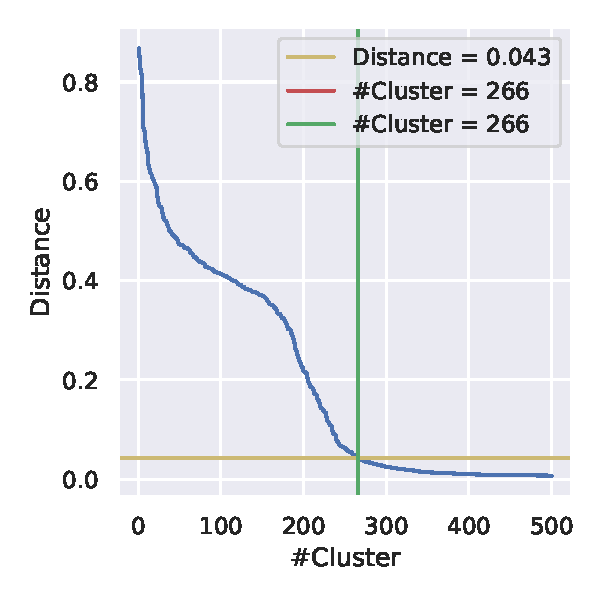
\includegraphics[width=\textwidth]{UMAP/Cluster_Elbow_Knee_Segment_4.pdf}
            \caption[Kneedle Knee]{\textbf{Kneedle Knee}}
            \label{fig:3.1.3b}
        \end{subfigure}
        \vskip\baselineskip
        \begin{subfigure}[b]{0.475\textwidth}
            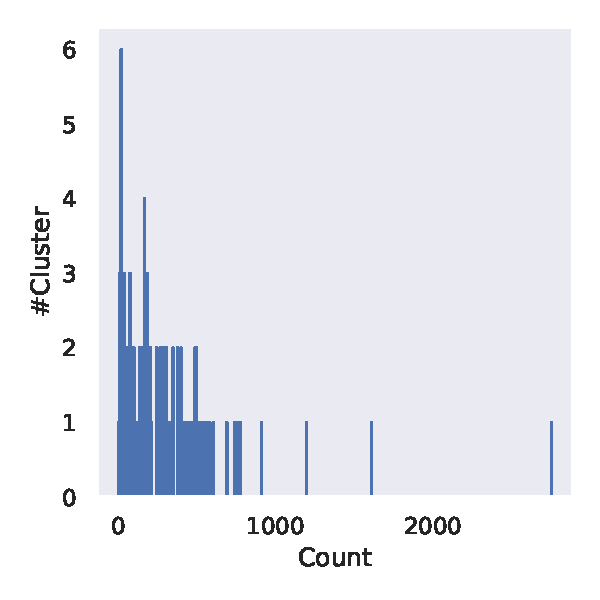
\includegraphics[width=\textwidth]{UMAP/Cluster_Distribution_Segment_4.pdf}
            \caption[Cluster Distribution]{\textbf{Cluster Distribution}}
            \label{fig:3.1.3c}
        \end{subfigure}
        \hfill
        \begin{subfigure}[b]{0.475\textwidth}
            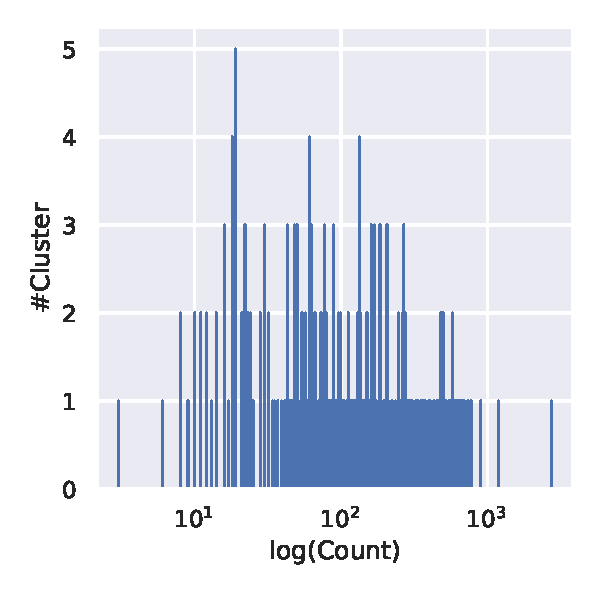
\includegraphics[width=\textwidth]{UMAP/Cluster_Distribution_Log_Segment_4.pdf}
            \caption[Logarithmic Distribution]{\textbf{Logarithmic Distribution}}
            \label{fig:3.1.3d}
        \end{subfigure}
    \end{adjustbox}
    \caption[Knee based Segment 4 Clustering with UMAP]{\textbf{Knee based Segment 4 Clustering with UMAP.}.}
    \label{fig:3.1.3}
\end{figure}

\begin{figure}
    \begin{adjustbox}{minipage=\dimexpr\textwidth-2\fboxsep-2\fboxrule,fbox}
        \begin{subfigure}[b]{0.475\textwidth}
            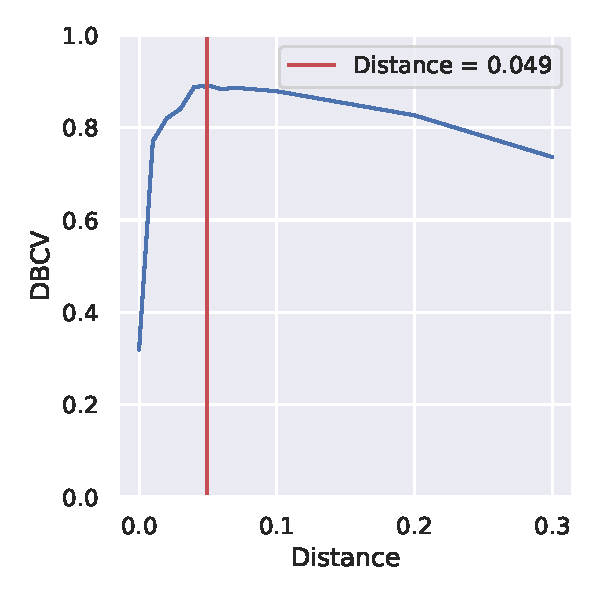
\includegraphics[width=\textwidth]{UMAP/Cluster_DBCV_Segment_4.pdf}
            \caption[DBCV Exploration]{\textbf{DBCV Exploration}}
            \label{fig:3.1.4a}
        \end{subfigure}
        \hfill
        \begin{subfigure}[b]{0.475\textwidth}
            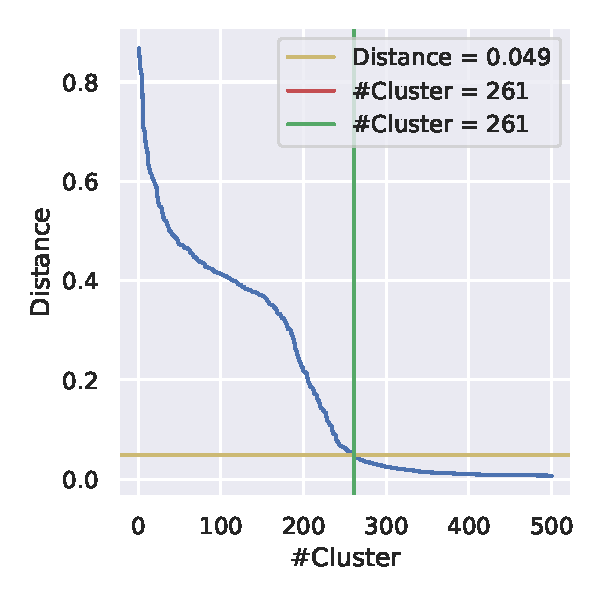
\includegraphics[width=\textwidth]{UMAP/Cluster_Elbow_DBCV_Segment_4.pdf}
            \caption[DBCV Knee]{\textbf{DBCV Knee}}
            \label{fig:3.1.4b}
        \end{subfigure}
        \vskip\baselineskip
        \begin{subfigure}[b]{0.475\textwidth}
            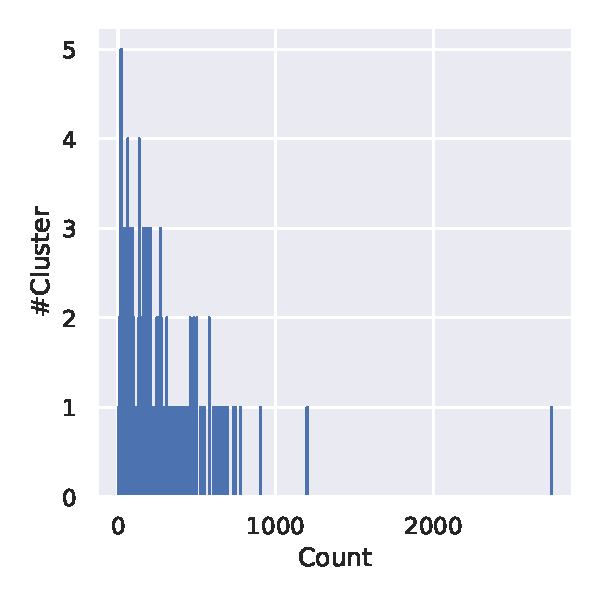
\includegraphics[width=\textwidth]{UMAP/Cluster_Distribution_Segment_4_alternative.pdf}
            \caption[Cluster Distribution]{\textbf{Cluster Distribution}}
            \label{fig:3.1.4c}
        \end{subfigure}
        \hfill
        \begin{subfigure}[b]{0.475\textwidth}
            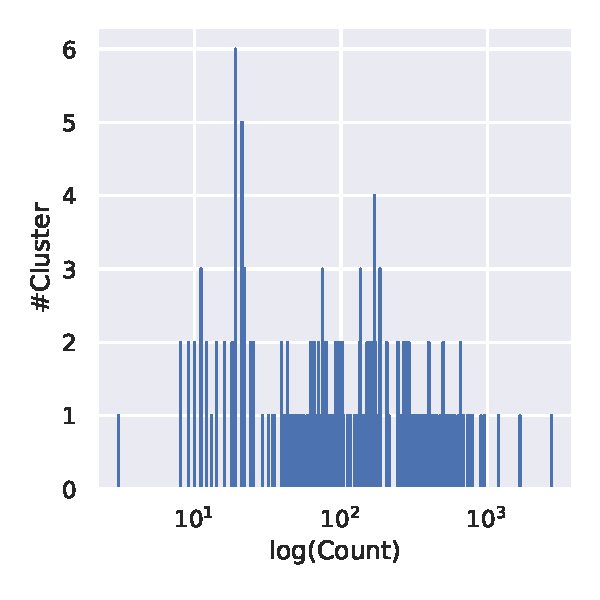
\includegraphics[width=\textwidth]{UMAP/Cluster_Distribution_Log_Segment_4_alternative.pdf}
            \caption[Logarithmic Distribution]{\textbf{Logarithmic Distribution}}
            \label{fig:3.1.4d}
        \end{subfigure}
    \end{adjustbox}
    \caption[DBCV based Segment 4 Clustering with UMAP]{\textbf{DBCV based Segment 4 Clustering with UMAP.}.}
    \label{fig:3.1.4}
\end{figure}

\begin{table}[!hbt]
    \caption[Knee based Clustering with PCA]{\textbf{Knee based Clustering with PCA.}.}
    \label{tab:3.1.1}
    \pgfplotstabletypeset[
        every head row/.style={
            before row={
                \toprule
                & \multicolumn{3}{l}{\textbf{Cluster}} &  & \multicolumn{2}{l}{\textbf{mixed}} &\\
                \cmidrule(lr){2-4}\cmidrule(lr){6-7}
            },
            after row={
                \midrule
            },
        },
        every last row/.style={
            after row={
                %... & ... & ... & ... & ... & ... & ... & ...\\
                \bottomrule
            },
        },
        begin table=\begin{tabular*}{\textwidth},
        end table=\end{tabular*},
        columns={0,1,2,3,4,5,6,7},
        columns/0/.style={multicolumn names=l,column name=\textbf{Segment}, column type=@{\extracolsep{\fill} }r},
        columns/1/.style={multicolumn names=l,column name=\textbf{\#Final}, column type=r},
        columns/2/.style={multicolumn names=l,column name=\textbf{\#Raw}, column type=r},
        columns/3/.style={multicolumn names=l,column name=\textbf{Normalized}, column type=r},
        columns/4/.style={multicolumn names=l,column name=\textbf{\#Unclustered}, column type=r},
        columns/5/.style={multicolumn names=l,column name=\textbf{H}, column type=r},
        columns/6/.style={multicolumn names=l,column name=\textbf{N}, column type=r},
        columns/7/.style={multicolumn names=l,column name=\textbf{Distance}, column type=r},
    ]
    {PCA/information.csv}
\end{table}

\begin{table}[!hbt]
    \caption[DBCV based Clustering with PCA]{\textbf{DBCV based Clustering with PCA.}.}
    \label{tab:3.1.2}
    \pgfplotstabletypeset[
        every head row/.style={
            before row={
                \toprule
                & \multicolumn{2}{l}{\textbf{Cluster}} &  & \multicolumn{2}{l}{\textbf{mixed}} & &\\
                \cmidrule(lr){2-3}\cmidrule(lr){5-6}
            },
            after row={
                \midrule
            },
        },
        every last row/.style={
            after row={
                %... & ... & ... & ... & ... & ... & ... & ...\\
                \bottomrule
            },
        },
        begin table=\begin{tabular*}{\textwidth},
        end table=\end{tabular*},
        columns={0,1,2,3,4,5,6,7},
        columns/0/.style={multicolumn names=l,column name=\textbf{Segment}, column type=@{\extracolsep{\fill} }r},
        columns/1/.style={multicolumn names=l,column name=\textbf{\#Final}, column type=r},
        columns/2/.style={multicolumn names=l,column name=\textbf{\#Raw}, column type=r},
        columns/3/.style={multicolumn names=l,column name=\textbf{\#Unclustered}, column type=r},
        columns/4/.style={multicolumn names=l,column name=\textbf{H}, column type=r},
        columns/5/.style={multicolumn names=l,column name=\textbf{N}, column type=r},
        columns/6/.style={multicolumn names=l,column name=\textbf{Distance}, column type=r},
        columns/7/.style={multicolumn names=l,column name=\textbf{DBCV}, column type=r},
    ]
    {PCA/information_alt.csv}
\end{table}

\begin{table}[!hbt]
    \caption[Knee based Clustering with UMAP]{\textbf{Knee based Clustering with UMAP.}.}
    \label{tab:3.1.3}
    \pgfplotstabletypeset[
        every head row/.style={
            before row={
                \toprule
                & \multicolumn{3}{l}{\textbf{Cluster}} &  & \multicolumn{2}{l}{\textbf{mixed}} &\\
                \cmidrule(lr){2-4}\cmidrule(lr){6-7}
            },
            after row={
                \midrule
            },
        },
        every last row/.style={
            after row={
                %... & ... & ... & ... & ... & ... & ... & ...\\
                \bottomrule
            },
        },
        begin table=\begin{tabular*}{\textwidth},
        end table=\end{tabular*},
        columns={0,1,2,3,4,5,6,7},
        columns/0/.style={multicolumn names=l,column name=\textbf{Segment}, column type=@{\extracolsep{\fill} }r},
        columns/1/.style={multicolumn names=l,column name=\textbf{\#Final}, column type=r},
        columns/2/.style={multicolumn names=l,column name=\textbf{\#Raw}, column type=r},
        columns/3/.style={multicolumn names=l,column name=\textbf{Normalized}, column type=r},
        columns/4/.style={multicolumn names=l,column name=\textbf{\#Unclustered}, column type=r},
        columns/5/.style={multicolumn names=l,column name=\textbf{H}, column type=r},
        columns/6/.style={multicolumn names=l,column name=\textbf{N}, column type=r},
        columns/7/.style={multicolumn names=l,column name=\textbf{Distance}, column type=r},
    ]
    {UMAP/information.csv}
\end{table}

\begin{table}[!hbt]
    \caption[DBCV based Clustering with PCA]{\textbf{DBCV based Clustering with PCA.}.}
    \label{tab:3.1.4}
    \pgfplotstabletypeset[
        every head row/.style={
            before row={
                \toprule
                & \multicolumn{2}{l}{\textbf{Cluster}} &  & \multicolumn{2}{l}{\textbf{mixed}} & &\\
                \cmidrule(lr){2-3}\cmidrule(lr){5-6}
            },
            after row={
                \midrule
            },
        },
        every last row/.style={
            after row={
                %... & ... & ... & ... & ... & ... & ... & ...\\
                \bottomrule
            },
        },
        begin table=\begin{tabular*}{\textwidth},
        end table=\end{tabular*},
        columns={0,1,2,3,4,5,6,7},
        columns/0/.style={multicolumn names=l,column name=\textbf{Segment}, column type=@{\extracolsep{\fill} }r},
        columns/1/.style={multicolumn names=l,column name=\textbf{\#Final}, column type=r},
        columns/2/.style={multicolumn names=l,column name=\textbf{\#Raw}, column type=r},
        columns/3/.style={multicolumn names=l,column name=\textbf{\#Unclustered}, column type=r},
        columns/4/.style={multicolumn names=l,column name=\textbf{H}, column type=r},
        columns/5/.style={multicolumn names=l,column name=\textbf{N}, column type=r},
        columns/6/.style={multicolumn names=l,column name=\textbf{Distance}, column type=r},
        columns/7/.style={multicolumn names=l,column name=\textbf{DBCV}, column type=r},
        %row predicate/.code={%
        %    \ifnum#1>0\relax
        %        \ifnum#1<2\relax
        %            \pgfplotstableuserowfalse
        %        \fi
        %    \fi
        %}
    ]
    {UMAP/information_alt.csv}
\end{table}

\blindtext

\begin{figure}[!hbt]

    \begin{annotatedFigure}
        {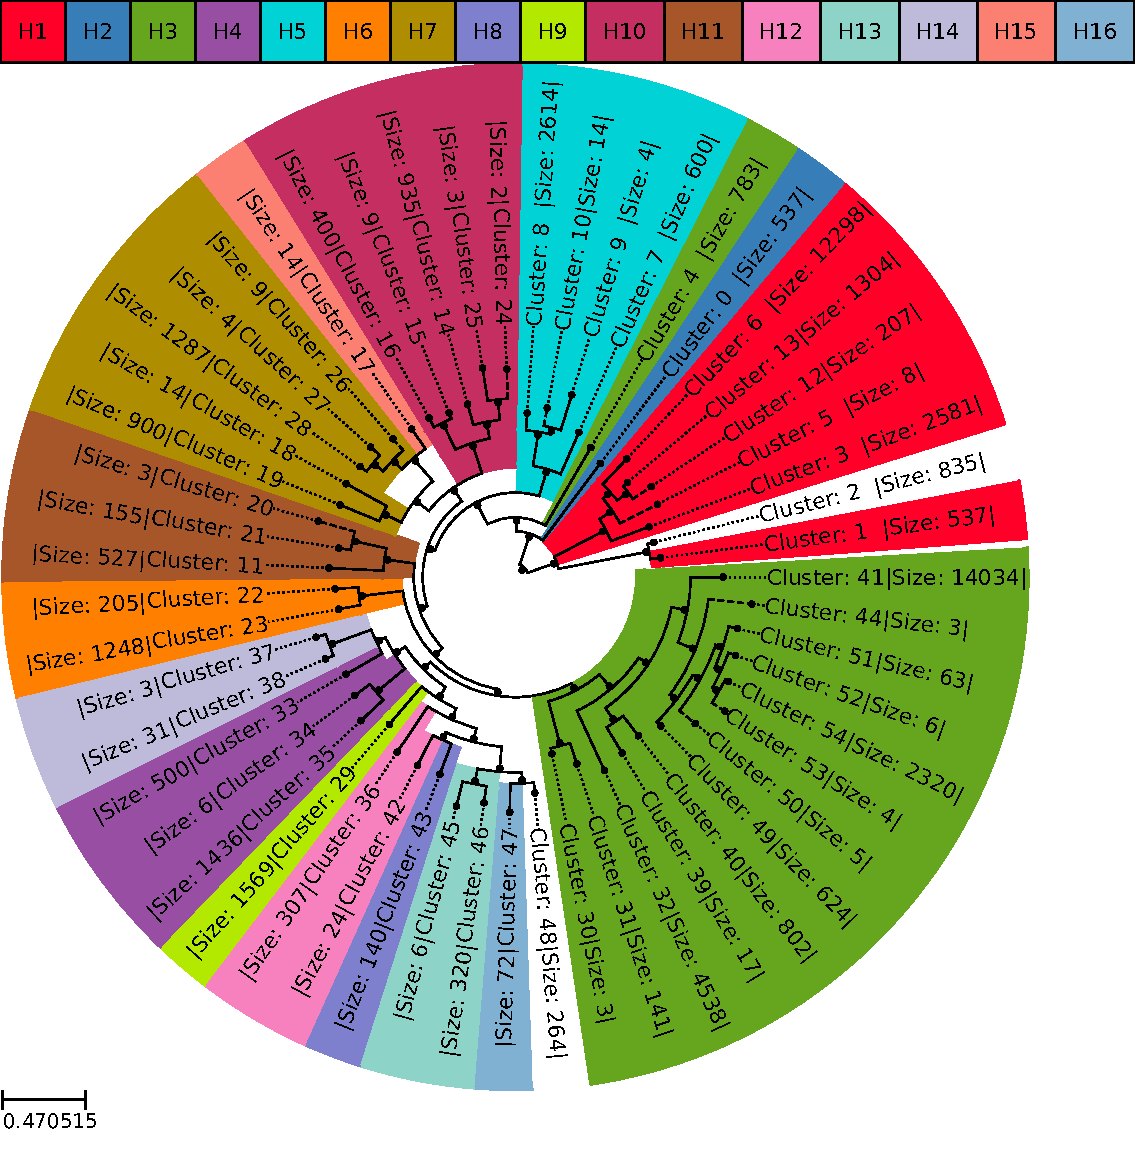
\includegraphics[width=\dimexpr\textwidth-2\fboxsep-2\fboxrule,fbox]{PCA/Clustertree_Segment_4_H_Knee.pdf}}
        \annotatedFigureBox{0.084,0.614}{0.394,0.804}{A}{0.084,0.614}%bl
    \end{annotatedFigure}
    
    \caption[Segment 4 Clustertree with PCA]{\textbf{Segment 4 Clustertree with PCA.} .}
    \label{fig:3.1.5}
\end{figure}

\begin{figure}[!hbt]
    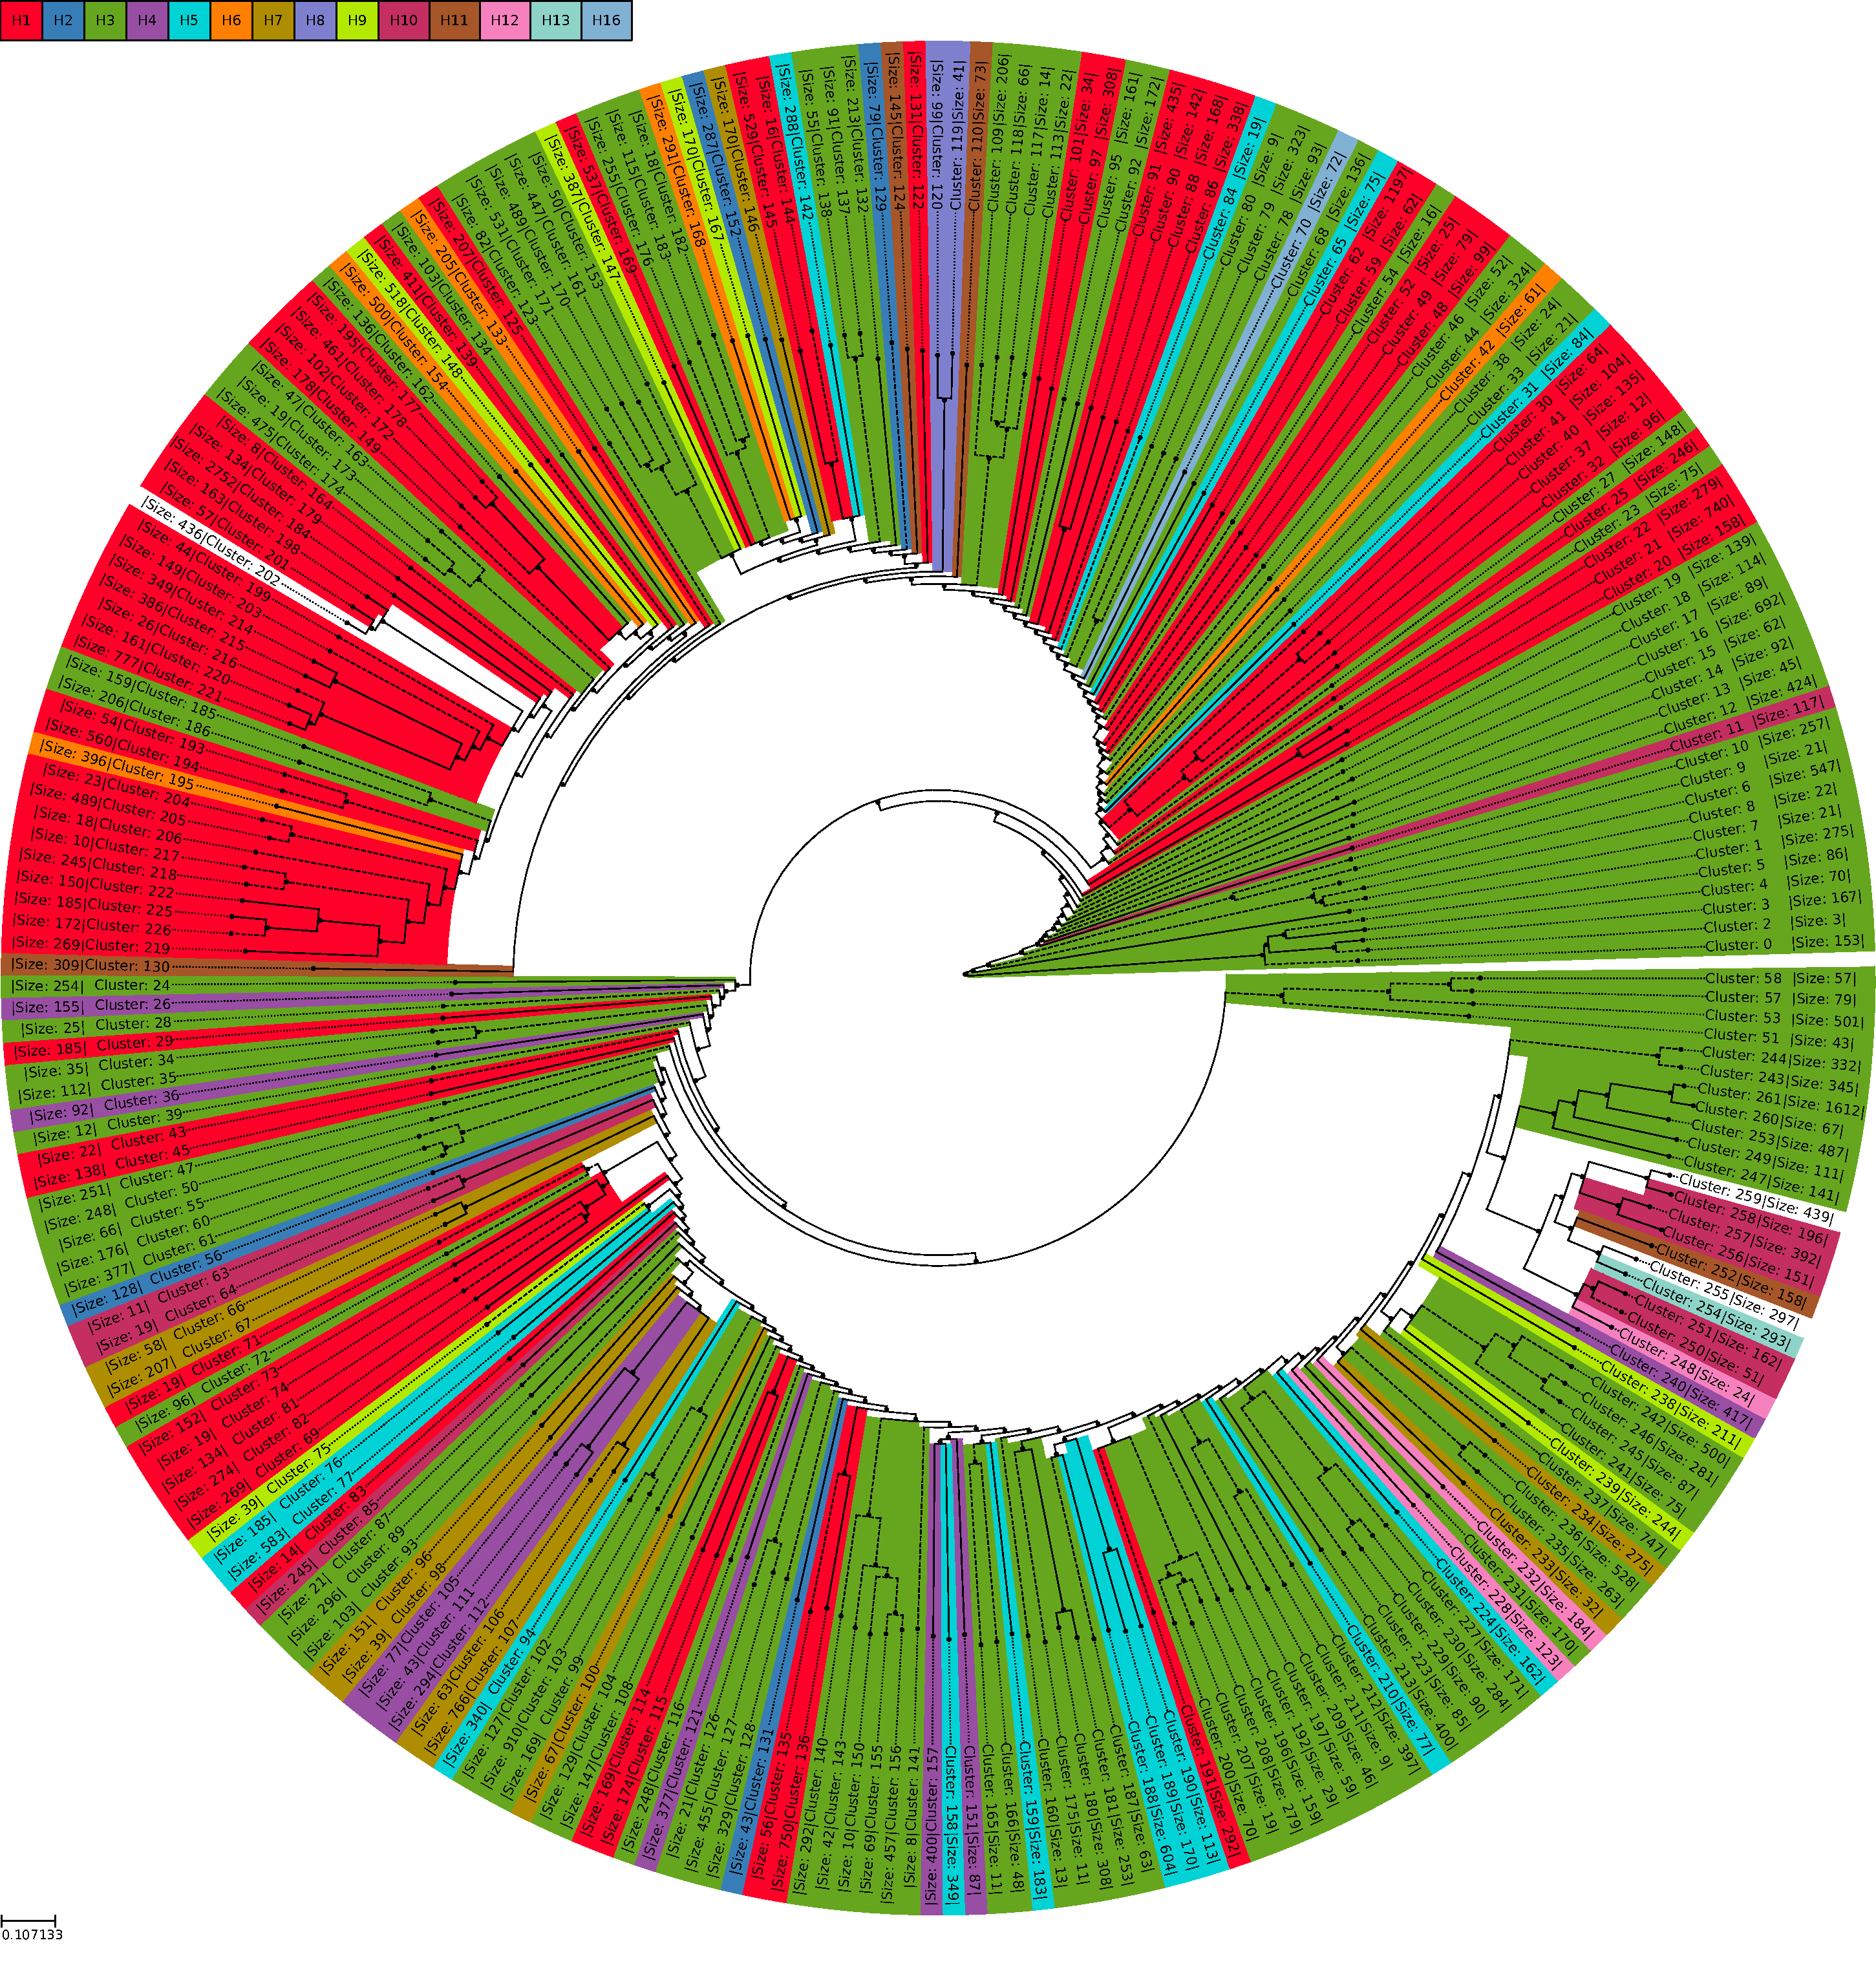
\includegraphics[width=\dimexpr\textwidth-2\fboxsep-2\fboxrule,fbox]{UMAP/Clustertree_Segment_4_H_Knee.pdf}
    \caption[Segment 4 Clustertree with UMAP]{\textbf{Segment 4 Clustertree with UMAP.} .}
    \label{fig:3.1.6}
\end{figure}

\section{Clustering Anomalies} \label{sec:Clustering_Anomalies}

\subsection{Clustering Errors}

\blindtext

\begin{table}[!hbt]
    \centering
    \caption[Anomalies in Segment 4 Cluster 2 (\Acrshort{PCA})]{\textbf{Anomalies in Segment 4 Cluster 2 (\Acrshort{PCA}).}.}
    \label{tab:PCA_Error_4_2}
    \pgfplotstabletypeset[
        every head row/.style={
            before row={
                \toprule
            },
            after row={
                \midrule
            },
        },
        every last row/.style={
            after row={
                %... & ... & ... & ... & ... & ... & ... & ...\\
                \bottomrule
            },
        },
        begin table=\begin{tabular*}{0.75\textwidth},
        end table=\end{tabular*},
        columns={0,1,2},
        columns/0/.style={string type,multicolumn names=l,column name=\textbf{Accession}, column type=@{\extracolsep{\fill}\hspace{6pt}}r},
        columns/1/.style={multicolumn names=l,column name=\textbf{H1}, column type=r},
        columns/2/.style={multicolumn names=l,column name=\textbf{H10}, column type=r},
    ]
    {PCA/error_segment_4_cluster_2_difference_head.csv}
\end{table}

\begin{table}[!hbt]
    \centering
    \caption[Anomalies in Segment 4 Cluster 48 (\Acrshort{PCA})]{\textbf{Anomalies in Segment 4 Cluster 48 (\Acrshort{PCA}).}.}
    \label{tab:PCA_Error_4_48}
    \pgfplotstabletypeset[
        every head row/.style={
            before row={
                \toprule
            },
            after row={
                \midrule
            },
        },
        every last row/.style={
            after row={
                ... & ... & ...\\
                \bottomrule
            },
        },
        begin table=\begin{tabular*}{0.75\textwidth},
        end table=\end{tabular*},
        columns={0,1,2},
        columns/0/.style={string type,multicolumn names=l,column name=\textbf{Accession}, column type=@{\extracolsep{\fill}\hspace{6pt}}r},
        columns/1/.style={multicolumn names=l,column name=\textbf{H16}, column type=r},
        columns/2/.style={multicolumn names=l,column name=\textbf{H13}, column type=r},
    ]
    {PCA/error_segment_4_cluster_48_difference_head.csv}
\end{table}

\begin{table}[!hbt]
    \centering
    \caption[Anomalies in Segment 4 Cluster 105 (\Acrshort{UMAP})]{\textbf{Anomalies in Segment 4 Cluster 105 (\Acrshort{UMAP}).}.}
    \label{tab:UMAP_Error_4_105}
    \pgfplotstabletypeset[
        every head row/.style={
            before row={
                \toprule
            },
            after row={
                \midrule
            },
        },
        every last row/.style={
            after row={
                \bottomrule
            },
        },
        begin table=\begin{tabular*}{0.75\textwidth},
        end table=\end{tabular*},
        columns={0,1,2},
        columns/0/.style={string type,multicolumn names=l,column name=\textbf{Accession}, column type=@{\extracolsep{\fill}\hspace{6pt}}r},
        columns/1/.style={multicolumn names=l,column name=\textbf{H1}, column type=r},
        columns/2/.style={multicolumn names=l,column name=\textbf{H10}, column type=r},
    ]
    {UMAP/error_segment_4_cluster_105_difference_head.csv}
\end{table}

\begin{table}[!hbt]
    \centering
    \caption[Anomalies in Segment 4 Cluster 265 (\Acrshort{UMAP})]{\textbf{Anomalies in Segment 4 Cluster 265 (\Acrshort{UMAP}).}.}
    \label{tab:UMAP_Error_4_265}
    \pgfplotstabletypeset[
        every head row/.style={
            before row={
                \toprule
            },
            after row={
                \midrule
            },
        },
        every last row/.style={
            after row={
                ... & ... & ... & ...\\
                \bottomrule
            },
        },
        begin table=\begin{tabular*}{0.75\textwidth},
        end table=\end{tabular*},
        columns={0,1,2,3},
        columns/0/.style={string type,multicolumn names=l,column name=\textbf{Accession}, column type=@{\extracolsep{\fill}\hspace{6pt}}r},
        columns/1/.style={multicolumn names=l,column name=\textbf{H7}, column type=r},
        columns/2/.style={multicolumn names=l,column name=\textbf{H10}, column type=r},
        columns/3/.style={multicolumn names=l,column name=\textbf{H12}, column type=r},
    ]
    {UMAP/error_segment_4_cluster_265_difference_head.csv}
\end{table}

\subsection{Centroid Guidetrees}

\blindtext

\begin{figure}[!hbt]
    \centering
    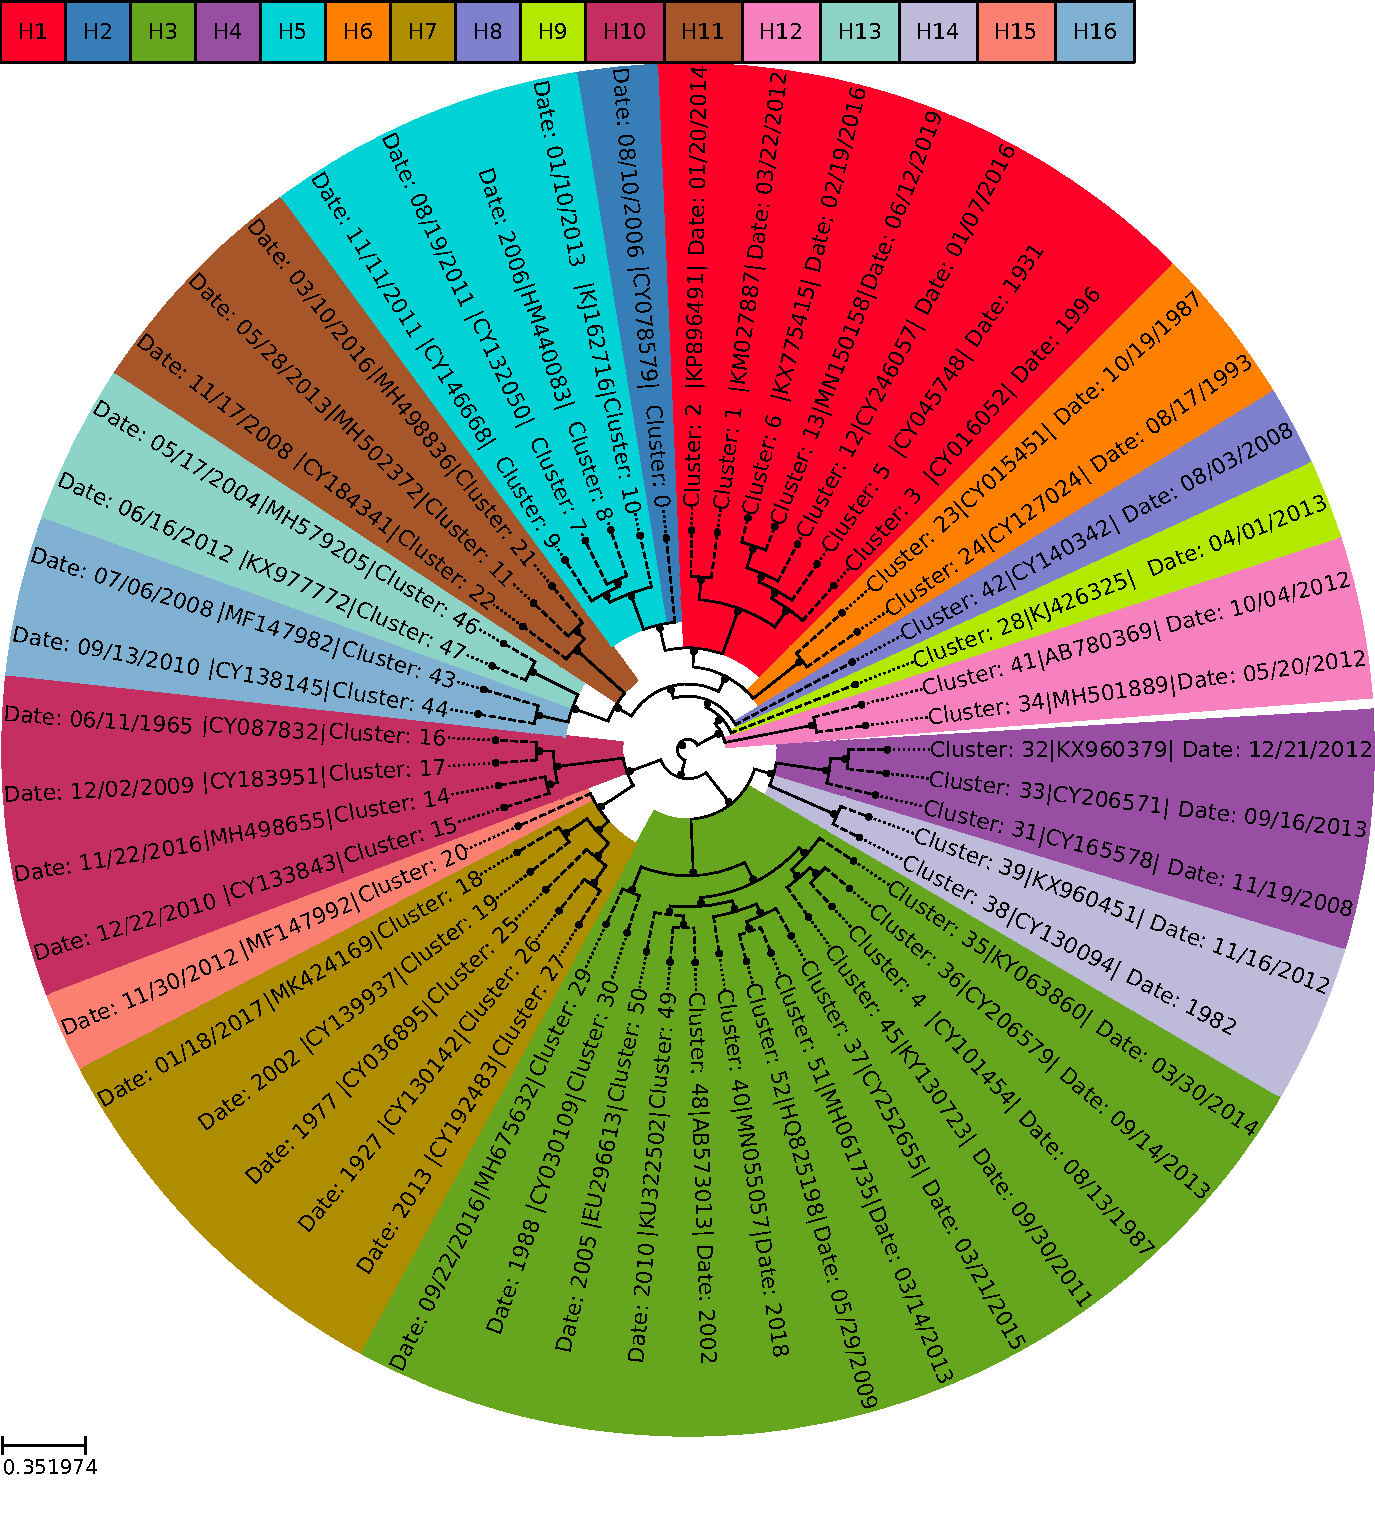
\includegraphics[width=\dimexpr\textwidth-2\fboxsep-2\fboxrule,fbox]{PCA/Guidetree_segment_4_H_Centroid.pdf}
    \caption[Knee based Segment 4 Centroid Guidetree (\Acrshort{PCA})]{\textbf{Knee based Segment 4 Centroid Guidetree (\Acrshort{PCA}).} .}
    \label{fig:PCA_Guidetree_Centroid_4}
\end{figure}

\blindtext

\begin{figure}[!hbt]
    \centering
    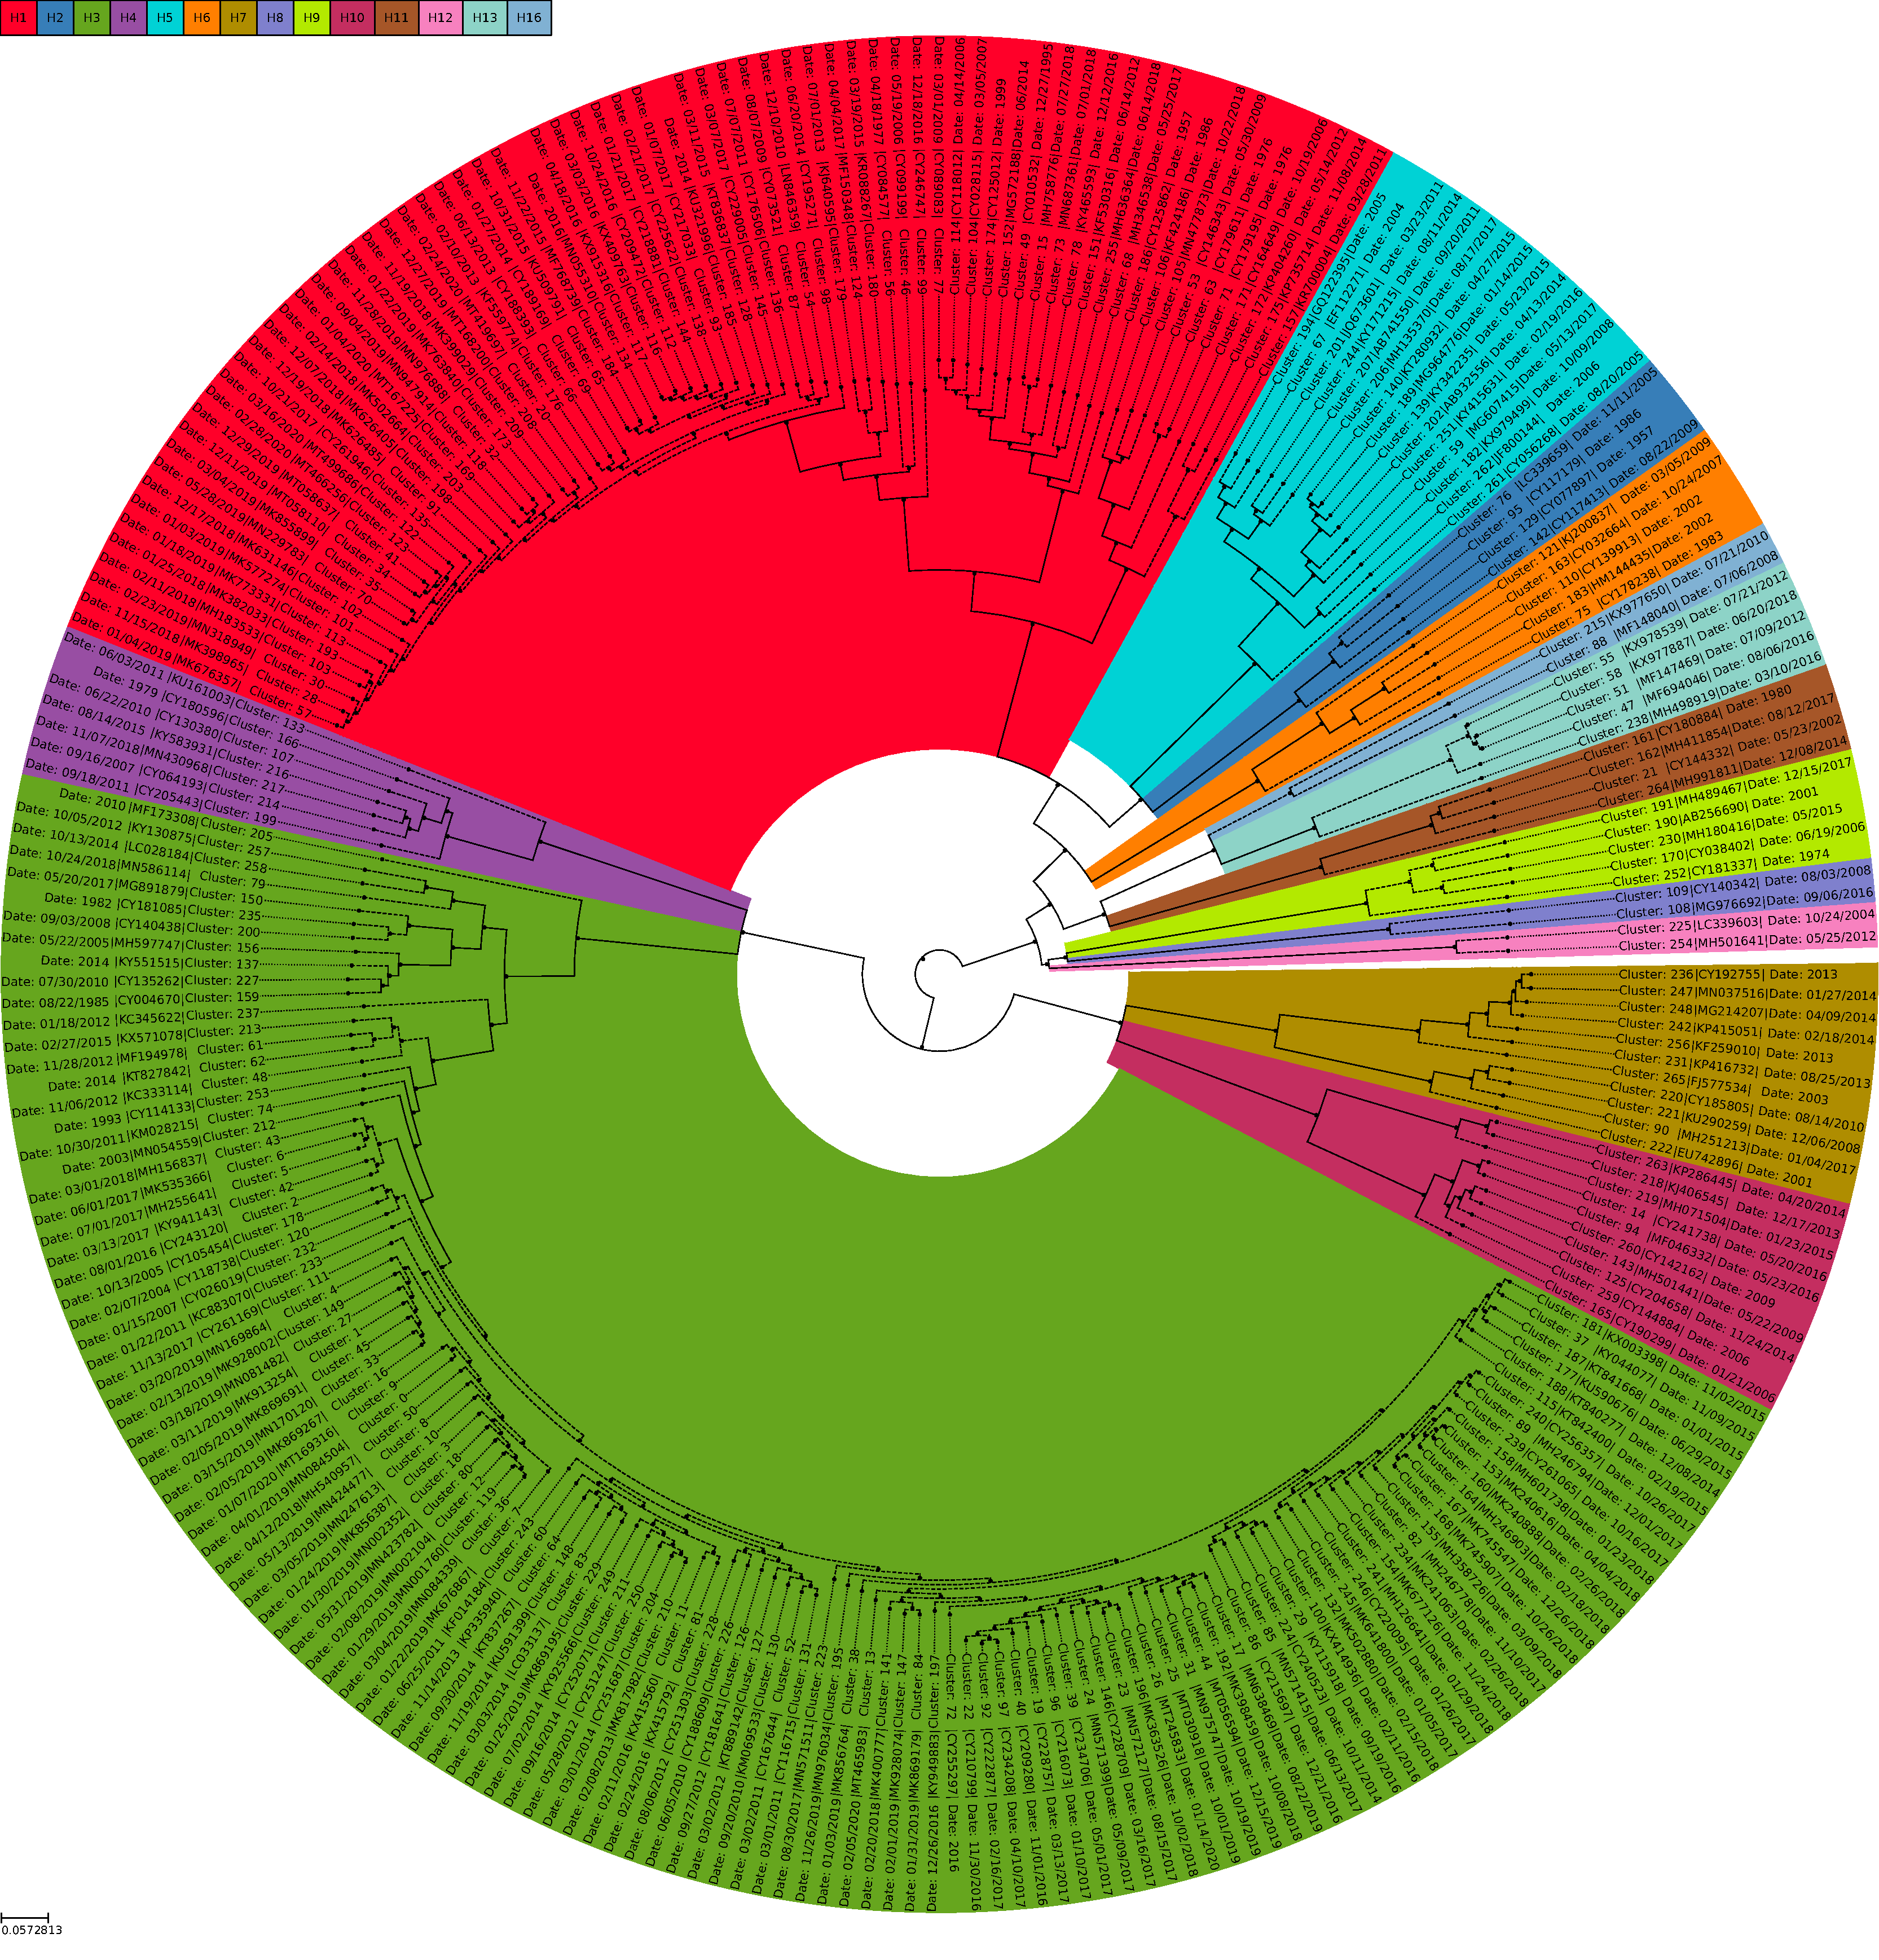
\includegraphics[width=\dimexpr\textwidth-2\fboxsep-2\fboxrule,fbox]{UMAP/Guidetree_segment_4_H_Centroid.pdf}
    \caption[Knee based Segment 4 Centroid Guidetree (\Acrshort{UMAP})]{\textbf{Knee based Segment 4 Centroid Guidetree (\Acrshort{UMAP}).} .}
    \label{fig:UMAP_Guidetree_Centroid_4}
\end{figure}

%Übergang zu cluster Comparison durch Centroid Alignment Tree -> H13/H16 Clustertree, Alignmenttree Vergleich -> Cluster H13/H16 Comparison

\section{K-mer Representation Quality} \label{sec:K_mer_Representation}

Investigation on the anomalies resulted in two persistent clustering errors (\autoref{fig:PCA_Cluster_Knee_4} \textbf{\textsf{B}} and \textbf{\textsf{D}}). To evaluate if the method is suitable for the clustering of \gls{IAV} possible error sources are discussed.

% \begin{figure}[!hbt]
%     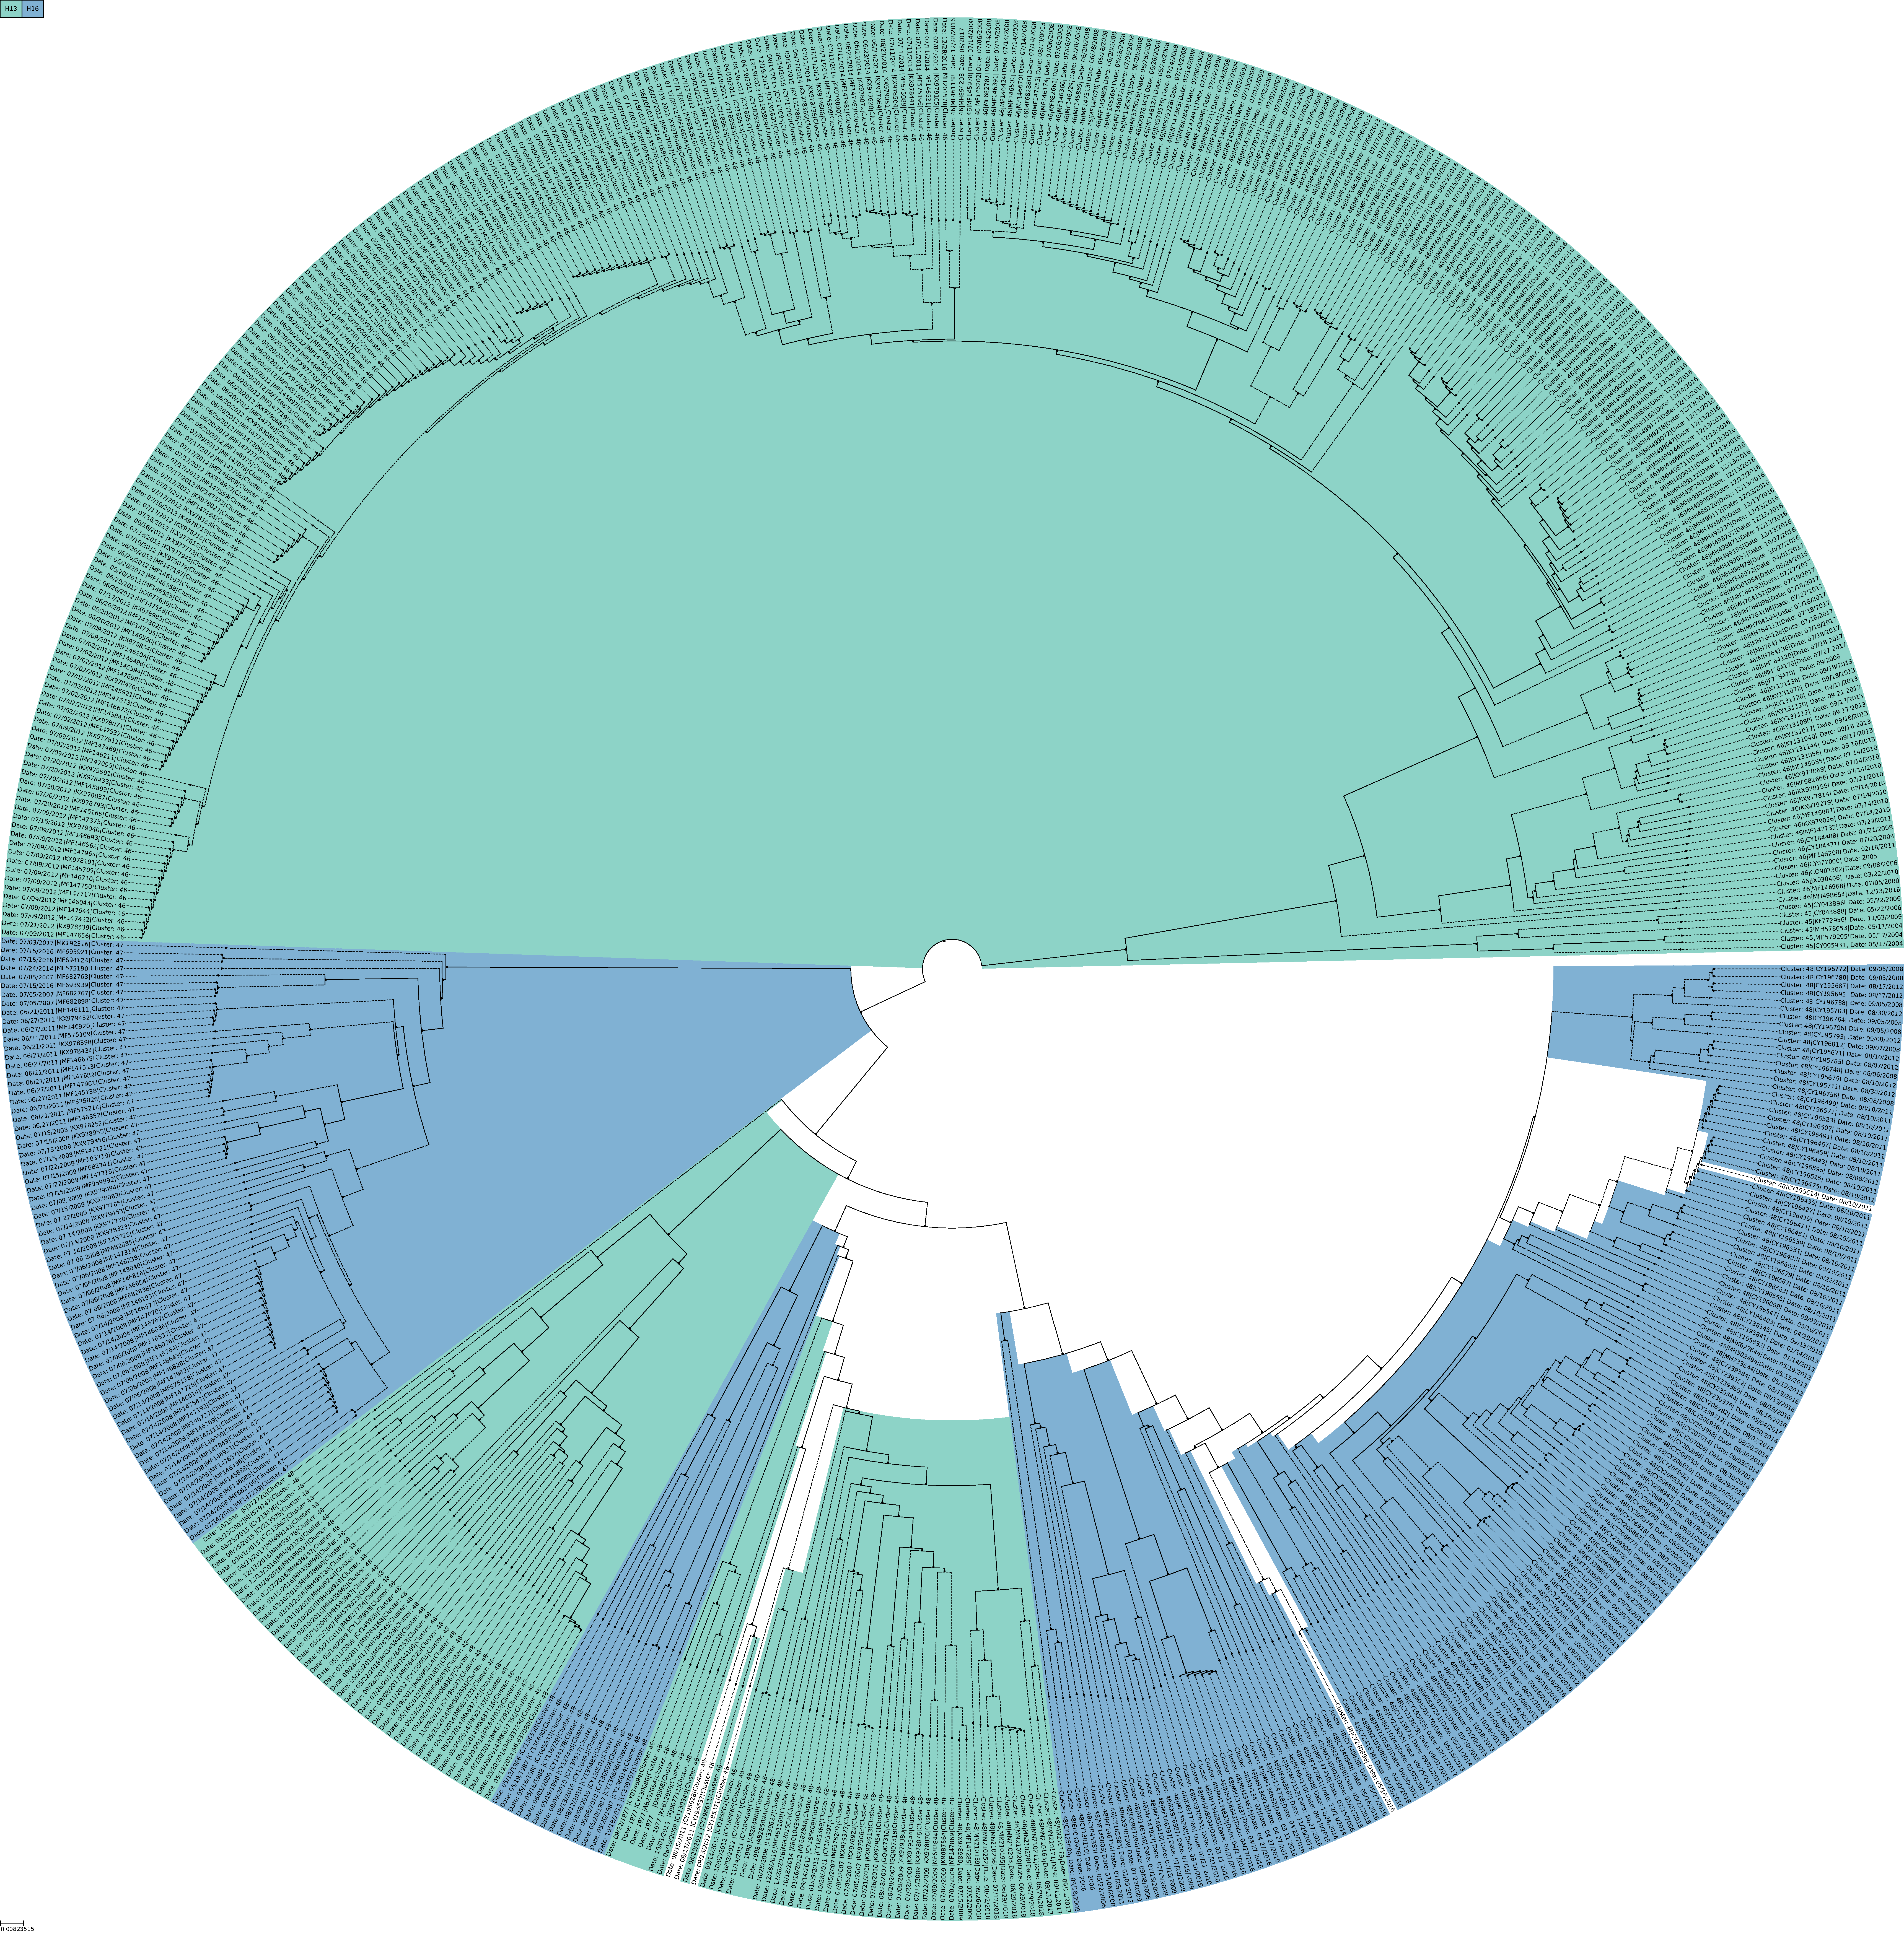
\includegraphics[width=\dimexpr\textwidth-2\fboxsep-2\fboxrule,fbox]{PCA/Clustertree_Segment_4_H_Knee_Zoom.pdf}
%     \caption[H13/H16 Simple Clustering Example with \Acrshort{PCA}]{\textbf{H13/H16 Simple Clustering Example with \Acrshort{PCA}.} .}
%     \label{fig:PCA_Clusteree_Knee_Zoom}
% \end{figure}

% \begin{figure}[!hbt]
%     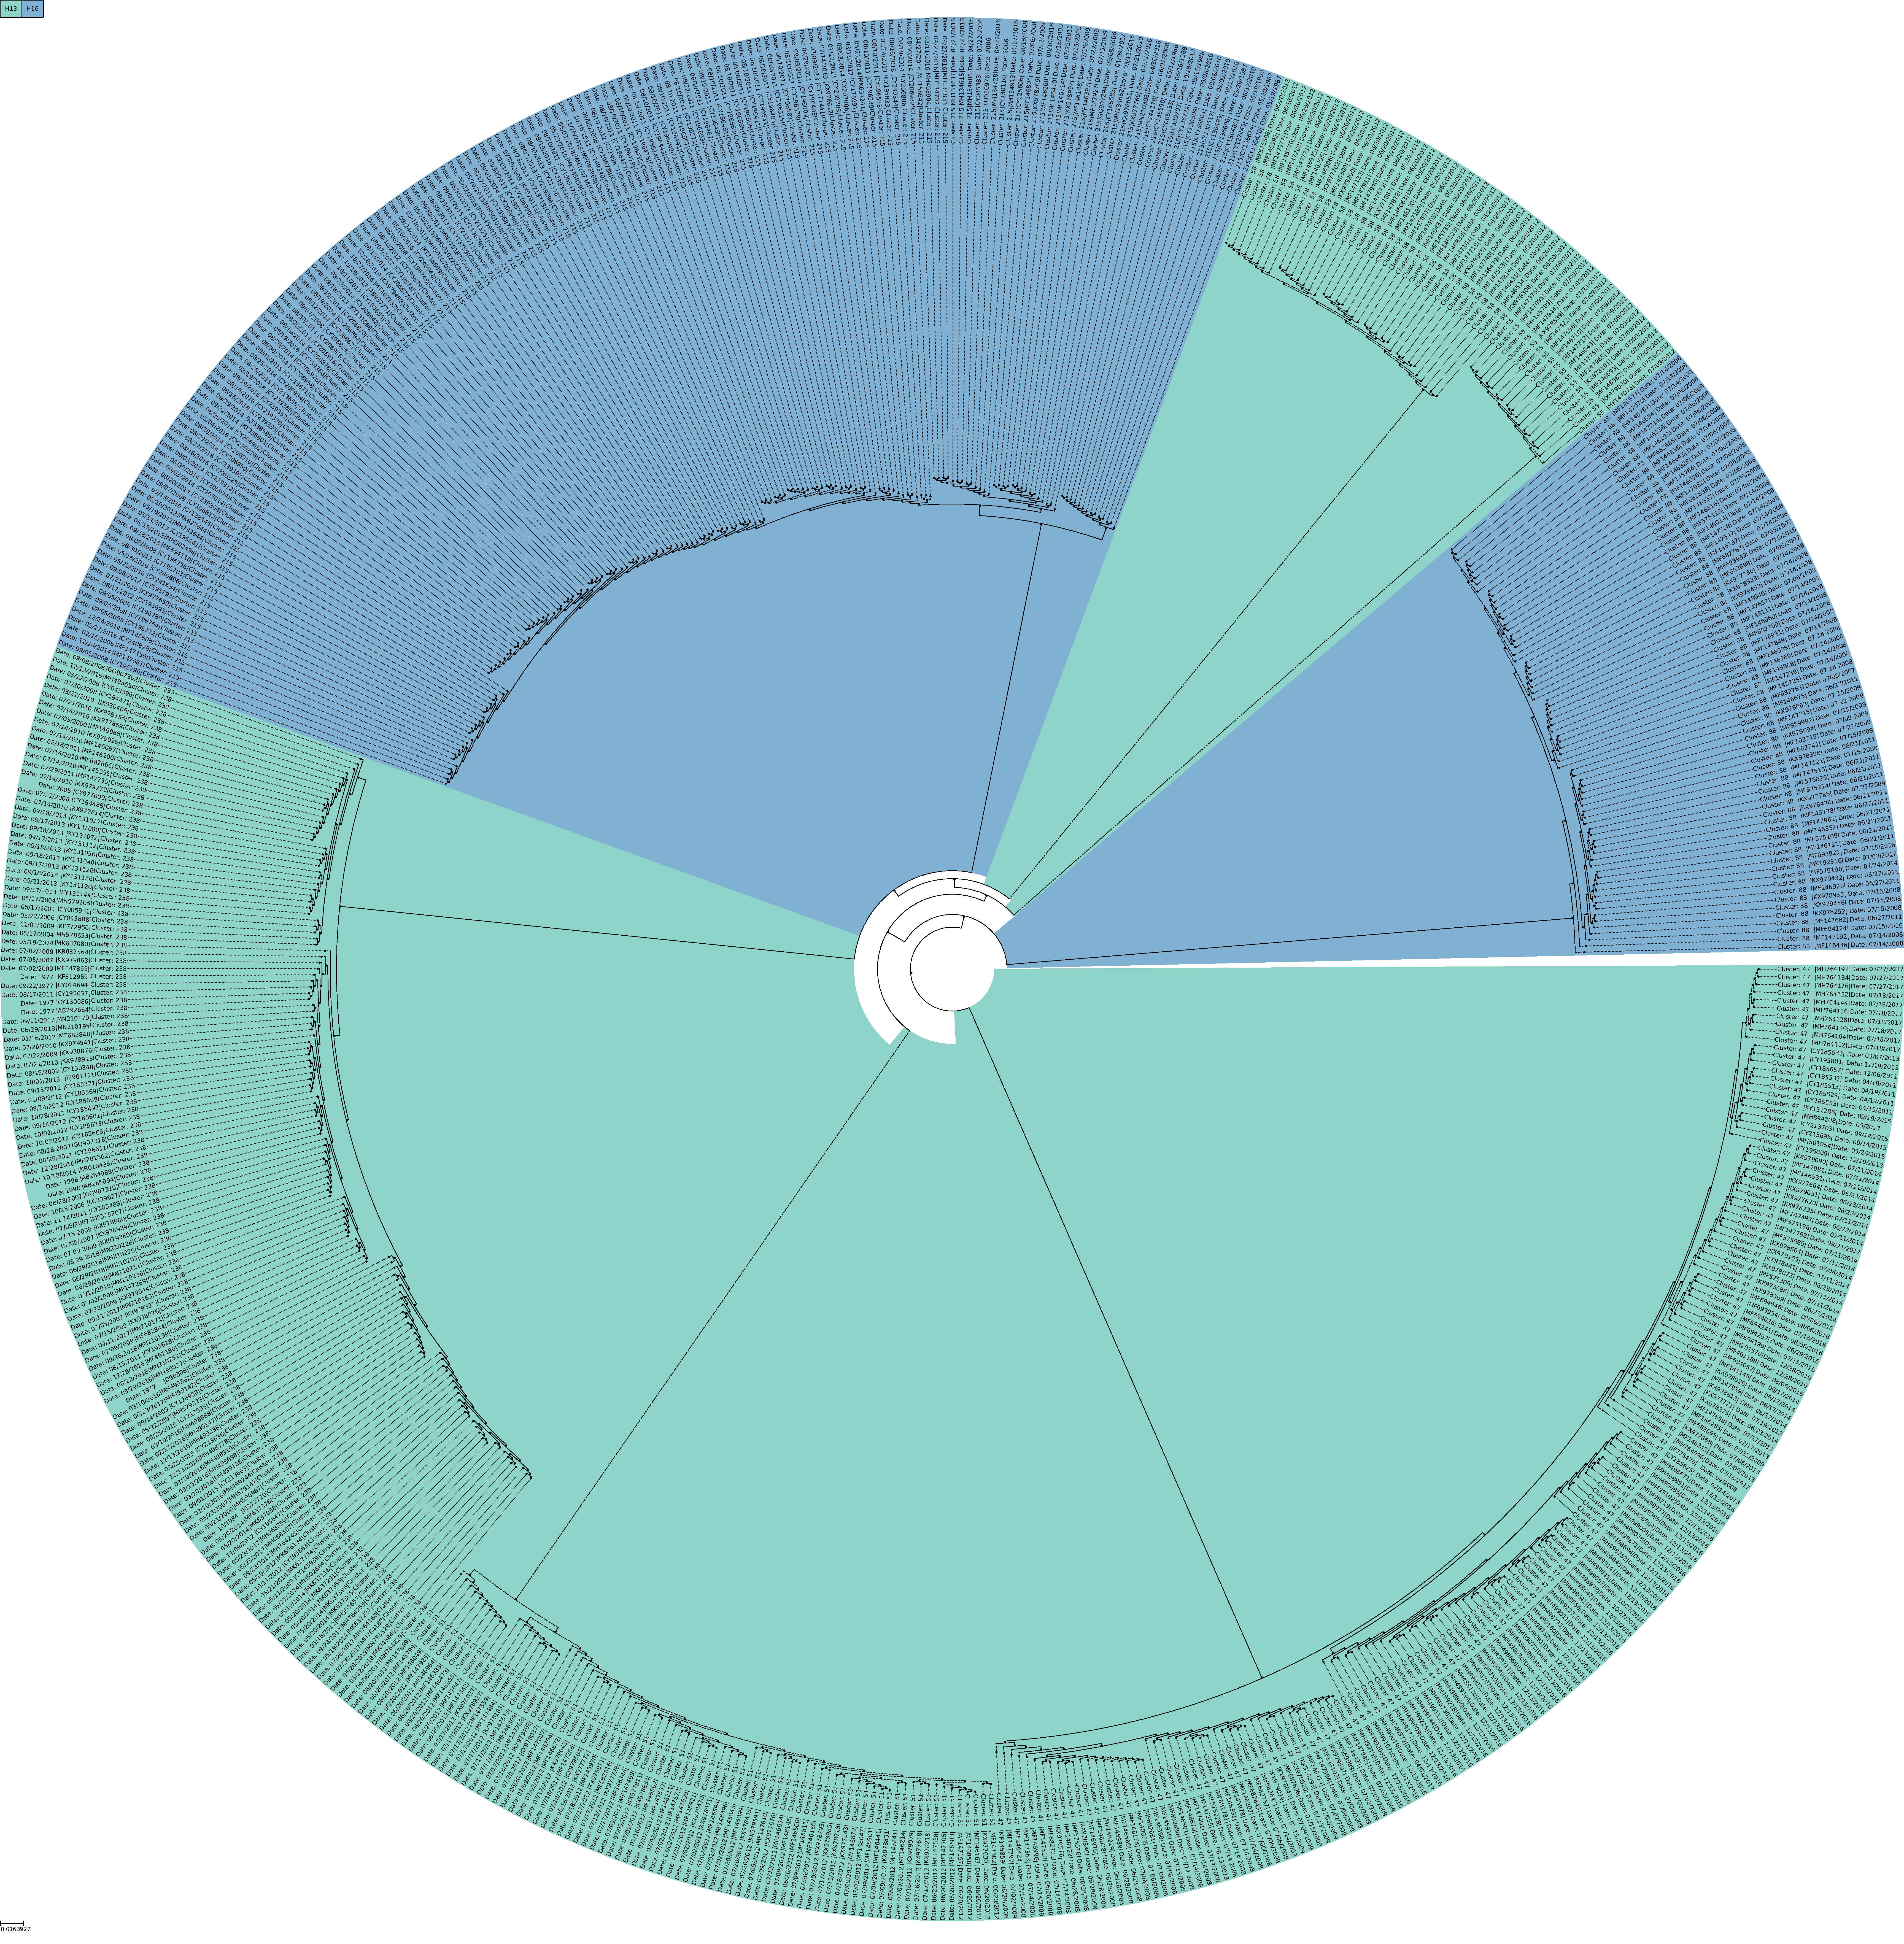
\includegraphics[width=\dimexpr\textwidth-2\fboxsep-2\fboxrule,fbox]{UMAP/Clustertree_Segment_4_H_Knee_Zoom.pdf}
%     \caption[H13/H16 Simple Clustering Example with \Acrshort{UMAP}]{\textbf{H13/H16 Simple Clustering Example with \Acrshort{UMAP}.} .}
%     \label{fig:UMAP_Clusteree_Knee_Zoom}
% \end{figure}

% \begin{figure}[!hbt]
%     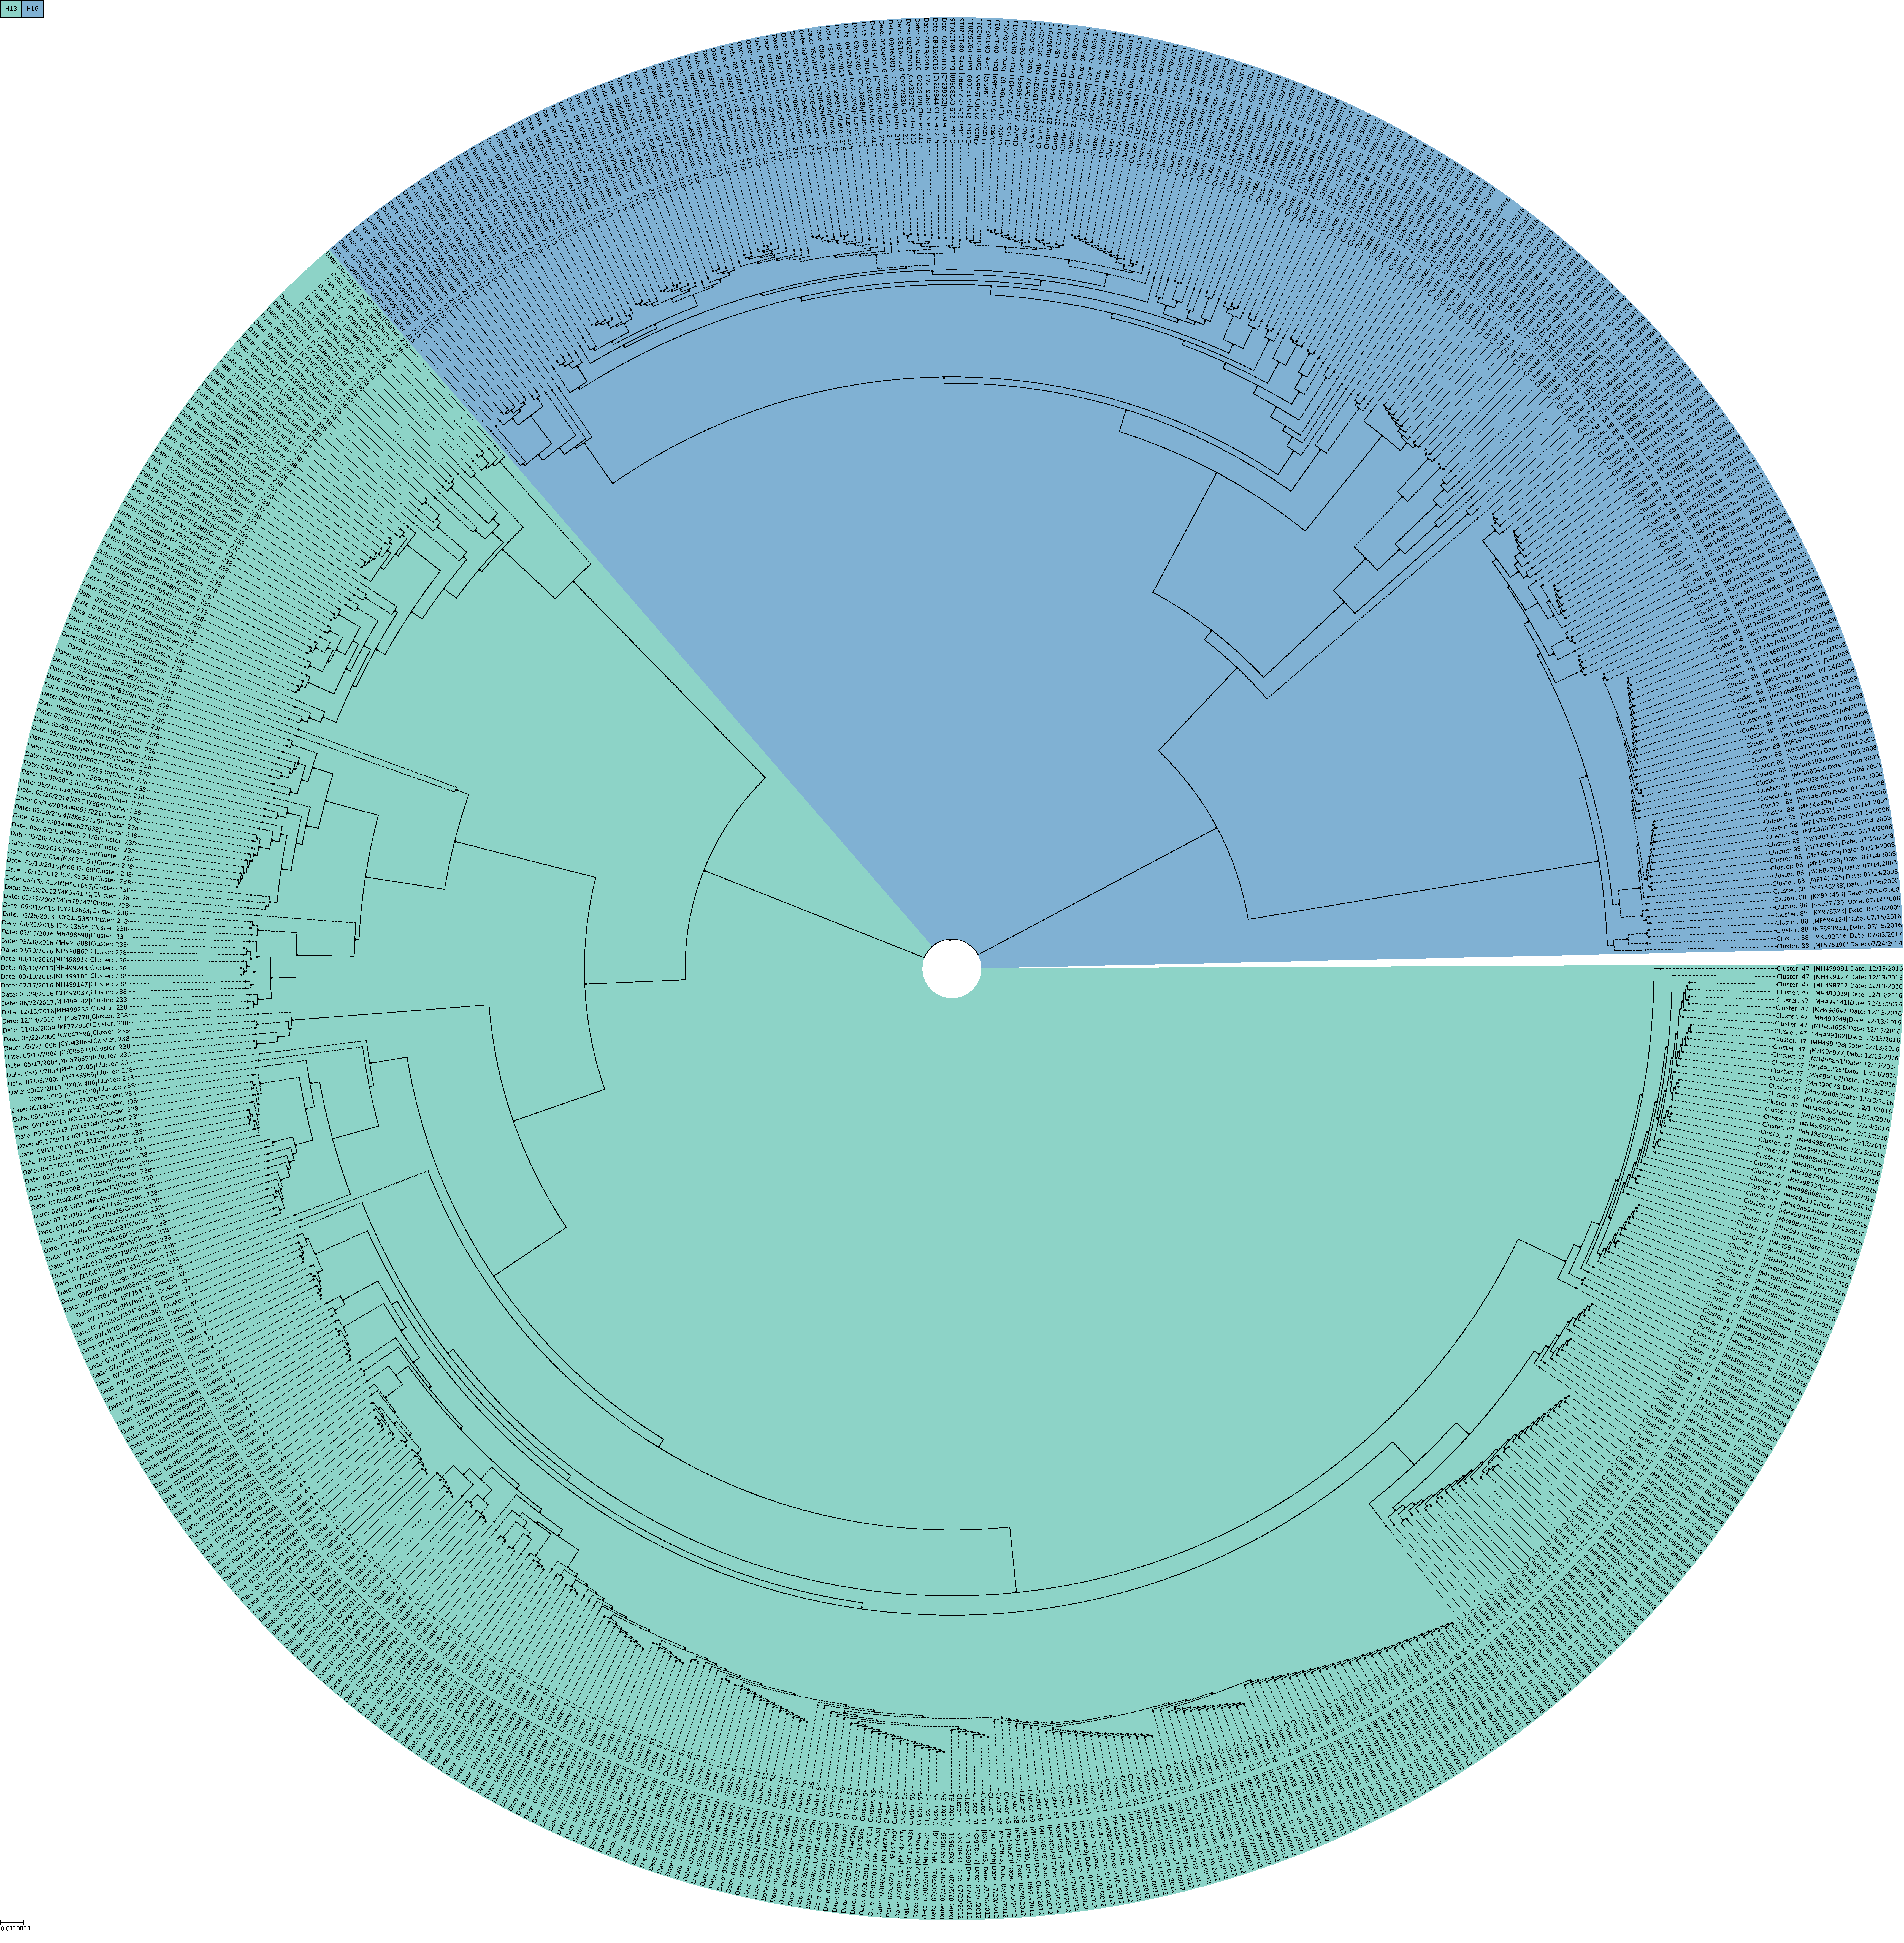
\includegraphics[width=\dimexpr\textwidth-2\fboxsep-2\fboxrule,fbox]{UMAP/Guidetree_Segment_4_H_Focus.pdf}
%     \caption[H13/H16 Simple Clustering Example with \Acrshort{MSA}]{\textbf{H13/H16 Simple Clustering Example with \Acrshort{MSA}.} .}
%     \label{fig:Guidetree_Focus}
% \end{figure}

\begin{figure}[!hbt]
    \centering
    \begin{tikzpicture}
        \node[anchor=south west,inner sep=0] (image) at (0,0) {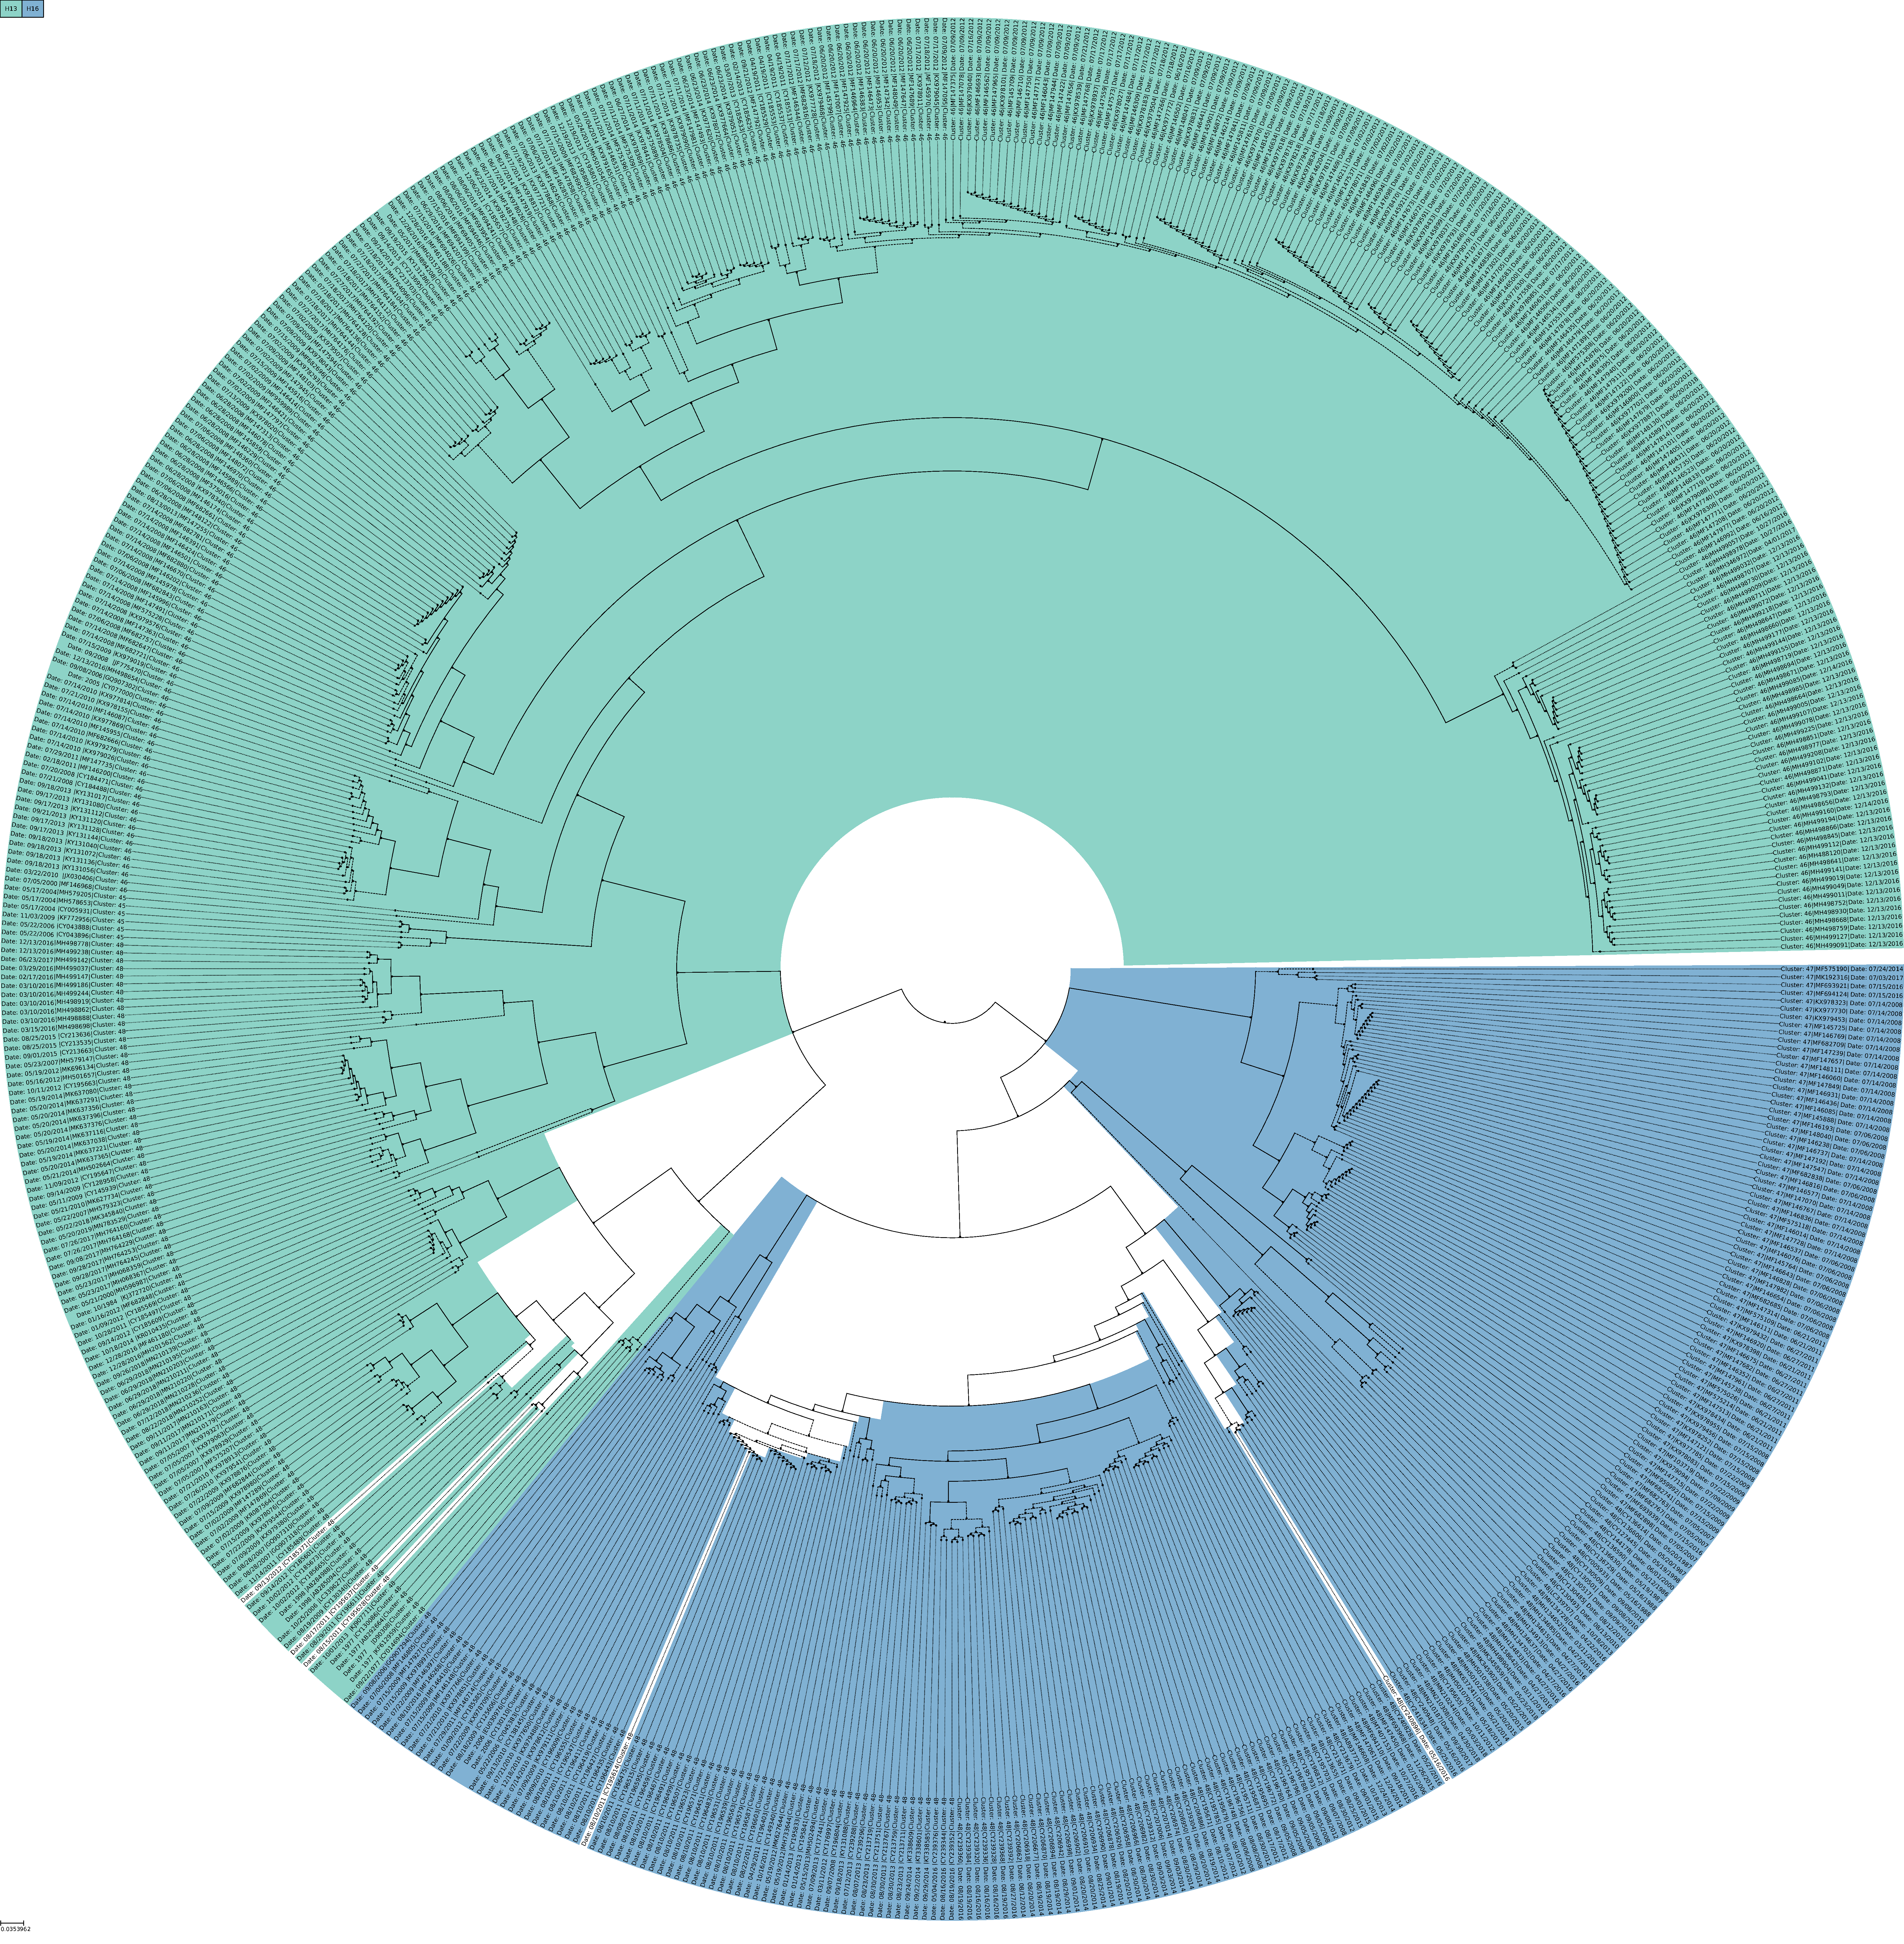
\includegraphics[width=\textwidth]{PCA/Precalculated_Segment_4_H_Cosine.pdf}};
        \begin{scope}[x={(image.south east)},y={(image.north west)}]
            %\draw[help lines,xstep=.1,ystep=.1] (0,0) grid (1,1);
            \draw[draw = none, fill = white] (0,1) rectangle (0.1,0.9);
            \draw[draw = none, fill = white] (0,0) rectangle (0.1,0.1);
            \draw[draw = black, thick, fill = black, fill opacity=0.0] (0.754,0.750) rectangle (0.999,0.505);
            \node at (0.754, 0.505) [fill=Red!80,thick,shape=circle,draw=black,inner sep=2pt] {\textbf{\textsf{C}}};
            %\draw[draw = black, thick, fill = black, fill opacity=0.2] (0.344, 0.603) rectangle (0.589,0.358);
            %\node at (0.344, 0.358) [fill=Red!80,thick,shape=circle,draw=black,inner sep=2pt] {\textbf{\textsf{A}}};
            \node at (0.425,0.525) [arrowstyle=1.5cm, arrowfillR, anchor=east, rotate=270] {\textbf{\textsf{A}}};
            \node at (0.55,0.525) [arrowstyle=1.5cm, arrowfillR, anchor=east, rotate=270] {\textbf{\textsf{B}}};
            %\draw[|-|] (0.975,0.5035) arc[start angle=0,end angle=170,radius=0.475, thick] node[midway,fill=Red!80,thick,shape=circle,draw=black,inner sep=2pt] {\textbf{\textsf{D}}};
            %\node at (0.5,0.505) [shape = circle,inner sep=140pt, fill = black] {};
            \node at (0.31,0.595) [arrowfillG, arrowstyle=1.5cm, anchor=east, rotate=315] {46};
            \node at (0.305,0.51) [arrowfillG, arrowstyle=1.5cm, anchor=east, rotate=45] {45};
            \node at (0.6,0.5) [arrowfillG, arrowstyle=1.5cm, anchor=east, rotate=225] {\rotatebox{180}{47}};
            \node at (0.35,0.455) [arrowfillG, arrowstyle=1.5cm, anchor=east, rotate=90] {48};
            \node at (0.425,0.42) [arrowfillG, arrowstyle=1.5cm, anchor=east, rotate=90] {48};
            \node at (0.54,0.435) [arrowfillG, arrowstyle=1.5cm, anchor=east, rotate=135] {\rotatebox{180}{48}};
        \end{scope}
    \end{tikzpicture}
    \caption[H13/H16 precalculated cosine distance \Acrshort{UPGMA} tree]{\textbf{H13/H16 precalculated cosine distance \Acrshort{UPGMA} tree.} Calculated cosine distance between the k-mer frequency vectors of sequences related to subtype H13 and H16 clusters in \autoref{fig:PCA_Clusteree_Knee_4} were used to build a \gls{UPGMA} tree. The same coloring of the previous tree was used to clarify the difference between H13 and H16 sequences. Uncolored sequences are unclassified ones from the inconclusive cluster 48 and, thereby, not assigned to a single subtype. The numbers in the green arrows indicate the cluster number of the sub trees sequences in \autoref{fig:PCA_Clusteree_Knee_4}. The red arrows are used in the following to point to the trees division into H13 \textbf{\textsf{A}} and H16 \textbf{\textsf{B}}. \autoref{fig:focus} is a enlarged view on the highlighted square at \textbf{\textsf{C}}.}
    \label{fig:Precalculated_Cosine}
\end{figure}

By building a \gls{UPGMA} tree on the non-reduced segment 4 k-mer frequency vectors of the H13 and H16 clusters 45, 46, 47 and 48, the unbiased relation of sequences from these subtypes were analyzed (\autoref{sec:MAFFT}). That way the fundamental use of k-mer frequencies was also validated. Not colored sequences are unclassified sequences (\autoref{fig:Frequency_4}) that also could not be assigned to a subtype, since they were clustered in a inconclusive cluster consisting of H13 and H16. Therefore, these sequences are unclassified sequences from cluster 48 (\autoref{fig:PCA_Clusteree_Knee_4} \textbf{\textsf{B}}).

\begin{figure}[!hbt]
    \centering
    %\begin{adjustbox}{minipage=\dimexpr\textwidth-2\fboxsep-2\fboxrule,fbox}
    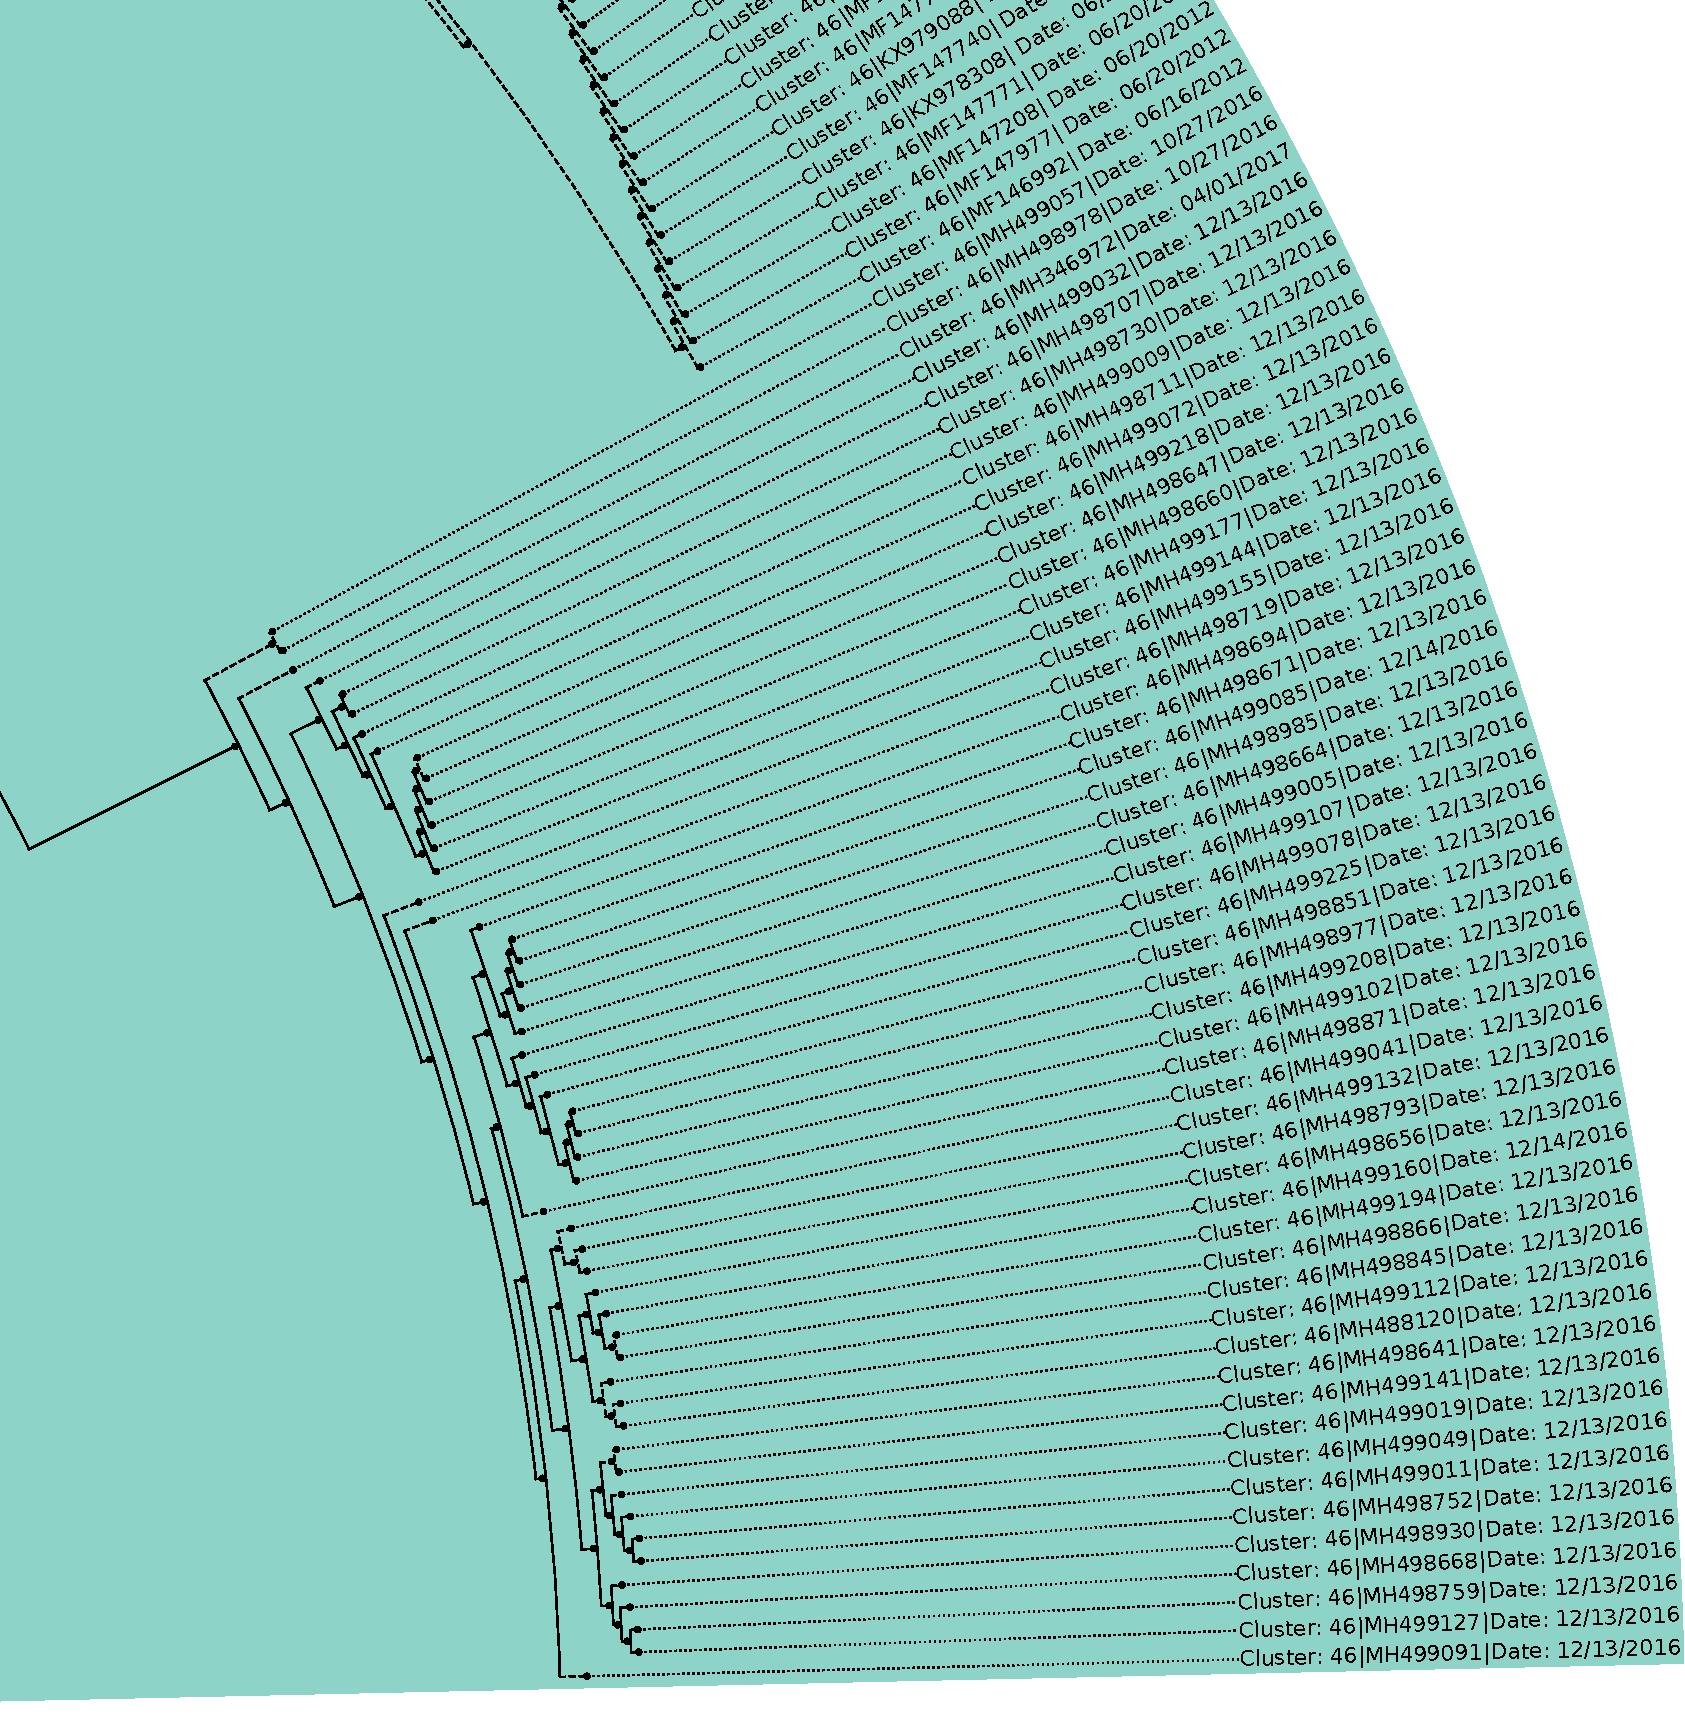
\includegraphics[width=\textwidth]{Graphics/identical.pdf}
    \caption[Relation of collection date and k-mer vector distance]{\textbf{Relation of collection date and k-mer vector distance.} Enlarged view of the by \textbf{\textsf{C}} highlighted square in \autoref{fig:Precalculated_Cosine}. The sequences were labeled according to their collection date to indicate the correlation of the close k-mer frequency vector distance in the tree with their sequences similarity. Labeling with the strain name could misleadingly point in a false direction, since the strain names indicate major difference while the sequences having very high similarity. Thereby the close distance of the vectors of sequences collected on the same date with high sequence similarity point to the precise representation by the k-mer frequency vectors.}
    \label{fig:focus}
\end{figure}

While both subtypes in \autoref{fig:Precalculated_Cosine} are completely separated directly after the trees root, there are also subdivisions for both subtypes directly after. This early subdivision can point to the existence of more subtle variations with major difference to each other than the existing subtype classification reveals. In this case it appears as if at least two subgroups for H13 and at least two or three subgroups for H16 exist. The threshold is difficult to define here and no clustering was performed in this case so this statement is based only on the early subdivision in the k-mer \gls{UPGMA}-tree (\autoref{fig:Precalculated_Cosine} \textbf{\textsf{A}} and \textbf{\textsf{B}}). The exact separation from the root is in line with the centroid guide-tree based on \gls{MSA} were both subtypes are completely separated too (\autoref{fig:PCA_Guidetree_Centroid_4}). Since this is also in line with the subtype classification, the k-mer frequency seems to work for this project. Furthermore, when focusing on a portion of the \gls{UPGMA}-tree with very small difference from sequence to sequence in \autoref{fig:Precalculated_Cosine} \textbf{\textsf{C}}, the similar collection date of all these sequences (12/13/2016) stand out. The only sequences not from this collection date but, nevertheless, included in this sub tree are MH499057, MH498978, MH346972, MH499085, and MH499160. Two of the first three mentioned sequences are from the same collection date but some days prior to the rest, while the third was collected some days after the 12/13/2016. These three sequences are the last linked sequences in the sub tree with the highest distance in comparison to the rest and their collection date is nearly the same as for the rest. The other two sequences with different date MH499085 and MH499160 are in the middle of the sub tree but the collected just one day after the rest. This points in the direction that even small differences are noticed by the k-mer approach. The collection date was used as comparison here because many of the sequences in the sub tree have very different strain names but are almost or completely similar and, thereby, could cause a misinterpretation. MH499085 of strain A/environment/Chile/C20369/2016 and MH498671 of strain A/white\_backed\_stilt/Chile/C20090/2016 differ by their strain names, as the virus was collected apparently completely different but the sequenced genomes are in fact 100\% the same. Around the tree in nearly every case similar collection dates have a small distance based on the k-mer frequency supporting the statement of the usability of k-mer frequencies for \gls{IAV} clustering. Same calculation for the precalculated \gls{UPGMA} tree was also repeated with euclidean distance and can be found in the \autoref{chap:Appendix}.

%frage is hier welche Methode die bessere representation ausstrahlt, sprich UMAP vgl. precalc ja/nein? dann PCA vgl precalc passt? ja/nein?

\section{Ground Truth for Clustering} \label{sec:Comparison_Clustering}

To further investigate in the source of the errors \autoref{fig:PCA_Cluster_Knee_4} \textbf{\textsf{B}} and \textbf{\textsf{D}}, \gls{HDBSCAN} was performed in a more simple manner, without $\varepsilon$ exploration on the small subset of H13 and H16 cluster of segment 4 in \autoref{fig:PCA_Clusteree_Knee_4}. Three different input matrices were used to compare the clustering by \gls{HDBSCAN} and find a ground truth. The first input was the non-reduced set of k-mer frequency vectors used in \autoref{sec:K_mer_Representation} as precalculated matrix with cosine distance (\autoref{sec:MAFFT}). Clustering was then performed and the result visualized as a cluster-tree (\autoref{fig:Simple_Clustertree_Cosine}). 

\begin{figure}[!hbt]
    \centering
    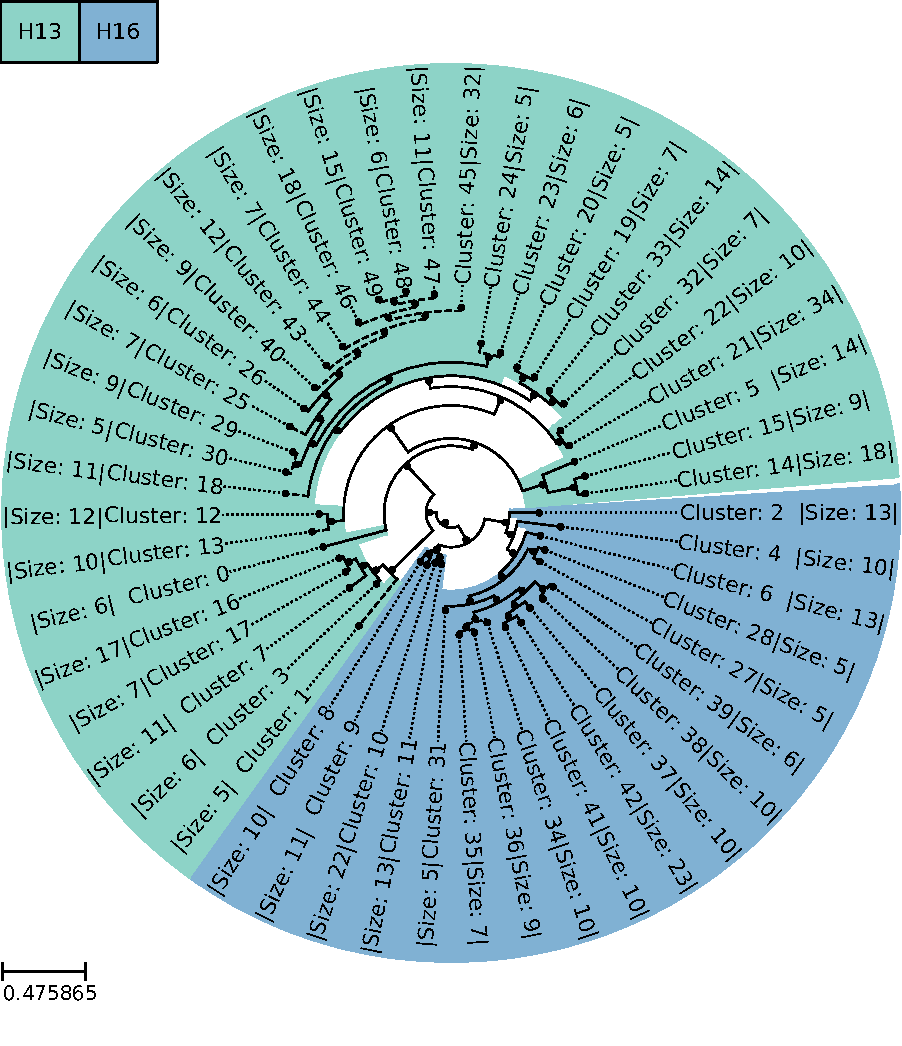
\includegraphics[width=\textwidth]{PCA/Clustertree_Segment_4_H_Cosine.pdf}
    \caption[H13/H16 simple precalculated cosine distance cluster tree]{\textbf{H13/H16 simple cosine distance cluster tree.} Cluster tree, based on the clustering by simple \gls{HDBSCAN} without any $\varepsilon$ exploration and hybrid clustering. The matrix used contained precalculated cosine distances of all the k-mer frequency vectors to each other. The used vectors were calculated from the sequences, present in the H13 and H16 clusters in \autoref{fig:PCA_Clusteree_Knee_4} without reduction with \gls{PCA} or \gls{UMAP}. Therefore, \gls{HDBSCAN} was used with precalculation input instead of a distance metric.}
    \label{fig:Simple_Clustertree_Cosine}
\end{figure}

\begin{figure}[!hbt]
    \centering
    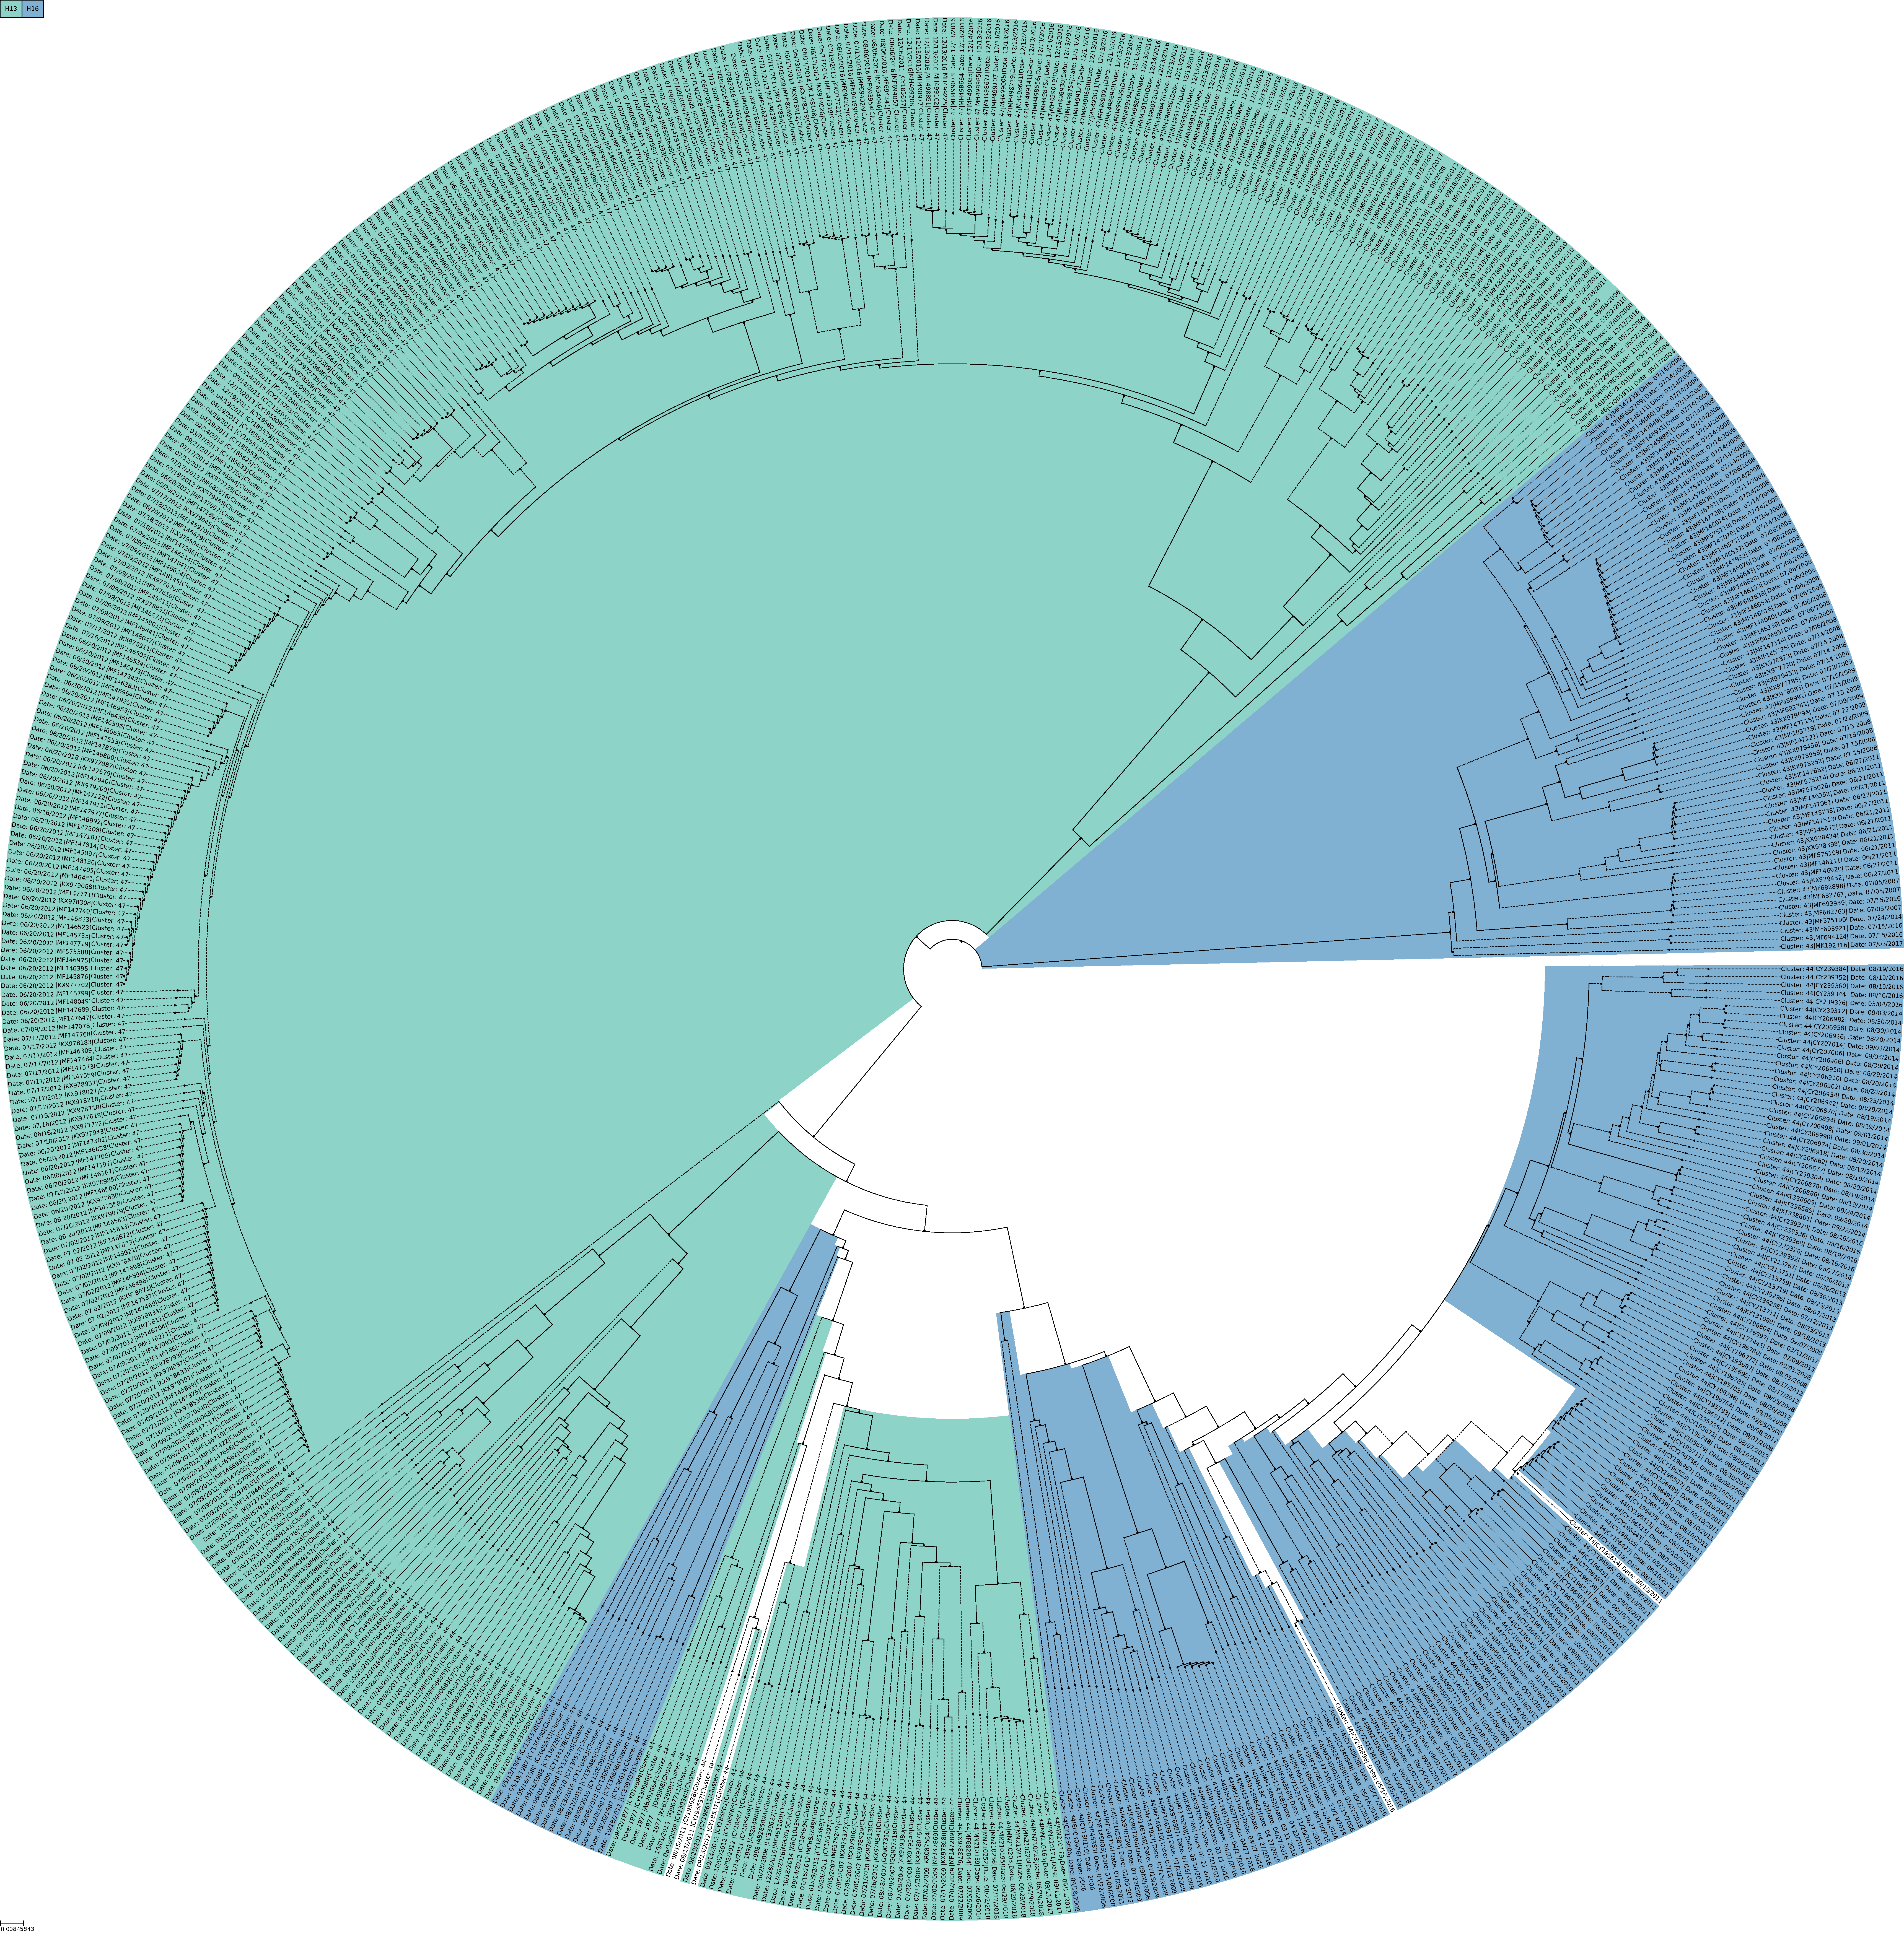
\includegraphics[width=\textwidth]{PCA/Clustertree_Segment_4_H_Focus.pdf}
    \caption[H13/H16 simple precalculated \gls{MSA} distance cluster tree]{\textbf{H13/H16 simple precalculated \gls{MSA} distance cluster tree.} Cluster tree, based on the clustering by simple \gls{HDBSCAN} without any $\varepsilon$ exploration and hybrid clustering. The matrix used contained precalculated \gls{MSA} based distances of all the sequences to each other. The sequences, present in the H13 and H16 clusters in \autoref{fig:PCA_Clusteree_Knee_4} were used for the \gls{MSA}. Therefore, \gls{HDBSCAN} was used with precalculation input instead of a distance metric.}
    \label{fig:Simple_Clustertree_MSA}
\end{figure}

\begin{figure}[!hbt]
    \centering
    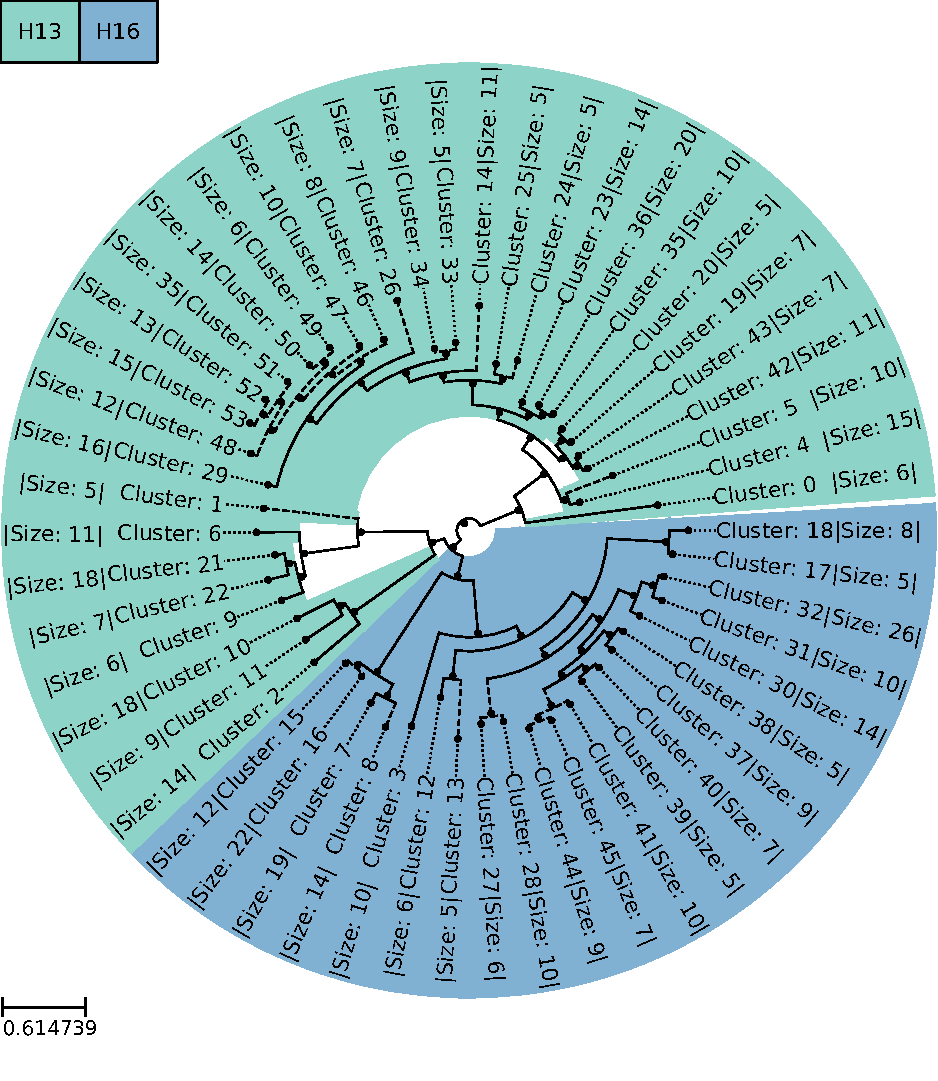
\includegraphics[width=\textwidth]{PCA/Clustertree_Segment_4_H_Simple.pdf}
    \caption[H13/H16 Simple \Acrshort{PCA} vector distance cluster tree]{\textbf{H13/H16 Simple \Acrshort{PCA} vector distance cluster tree.} Cluster tree, based on the clustering by simple \gls{HDBSCAN} without any $\varepsilon$ exploration and hybrid clustering. The used vectors were calculated from the sequences, present in the H13 and H16 clusters in \autoref{fig:PCA_Clusteree_Knee_4} with prior \gls{PCA} reduction to 30 dimensions.}
    \label{fig:Simple_Clustertree_PCA}
\end{figure}

In a similar manner to the precalculated \gls{UPGMA} tree in \autoref{fig:Precalculated_Cosine}, the subtypes are completely separated and split on both sides in two subgroups. This points to the fact, that the \gls{HDBSCAN} clustering of the precalculated cosine distances of the k-mer frequencies are as usable as the k-mer frequencies itself and are able to draw a clear line to separate the subtypes. This finding is in line with the second simple cluster-tree based on the evolutionary distances of a \gls{MSA} containing the same sequences as used in the former precalculated cosine distance clustering (\autoref{fig:Simple_Clustertree_MSA}). The same separation is even more obvious, as the subtypes are farther away from the separation at the trees root. On the side of the H13 sequences, a subdivision is also as clear as the subtype separation. Subgroups in the H16 sequences are, on the other hand, not that clear in \autoref{fig:Simple_Clustertree_MSA}. Maybe the different distances between the subtypes and the subgroups on each side of the subtypes is different because evolutionary aspects like weightings and different costs for nucleotides that are more likely to change are used. In the k-mer frequencies, the pure constellation of nucleotides is used, evolutionary aspects are neglected. Both, the precalculated approach as well as the \gls{MSA} evolutionary distances used the full information available from the sequences themselves, since no reduction with \gls{PCA} was performed. Therefore these cluster trees (\autoref{fig:Simple_Clustertree_Cosine} and \autoref{fig:Simple_Clustertree_MSA}) are the only ground truth for H13/H16 clustering with \gls{HDBSCAN} available. Precalculated clustering with \gls{HDBSCAN} as performed, is a highly computationally expensive task, as with $n$ sequences, the matrices of size $n^2$ have to be calculated and saved to be used in \gls{HDBSCAN}. The calculation is, therefore, not possible without the availability of major RAM space. When using \gls{HDBSCAN} with the k-mer vectors posterior to reduction with \gls{PCA} to 30 dimensions, only a matrix of size $n\times 30$ has to be saved without the necessity of any distance precalculation. To find a clustering method available without using hardware that offers extensive computational power, the simple cluster tree with \gls{PCA} should preferably resemble the previous cluster trees.

Unfortunately, some major differences between the simple cluster tree using \gls{PCA} and the previous precalculated trees using \gls{MSA} and cosine distances occurred (\autoref{fig:Simple_Clustertree_Cosine}, \autoref{fig:Simple_Clustertree_MSA} and \autoref{fig:Simple_Clustertree_PCA}). The same clustering behavior as in the complete cluster tree can be observed as no clear separation on the H13 and H16 clusters is present (\autoref{fig:Simple_Clustertree_PCA} and \autoref{fig:PCA_Clusteree_Knee_4} \textbf{\textsf{B}}). The simple clustering performed with \gls{MSA} distances and precalculated cosine distances showed a clear separation on the subtypes. Since the precalculated distances are solely based on the k-mer frequencies and the \gls{MSA} distances on the evolutionary aspect and both methods present a clear separation, the \gls{PCA} or dimension reduction step seems to be the origin of the clustering error in \autoref{fig:PCA_Cluster_Knee_4} \textbf{\textsf{B}} and \textbf{\textsf{D}}. 

As already mentioned the precalculated cluster trees use the whole available amount of information given by the sequences, either by direct use of the nucleotide comparisons with \gls{MSA} (\autoref{fig:Simple_Clustertree_MSA}) or by using the k-mer frequency vectors without reducing the dimension (\autoref{fig:Simple_Clustertree_Cosine}). Thus, the amount of information remaining in the vectors did not seem to suffice for the given task. The simple clustering was also performed with the same subset of H13 and H16 sequences reduced with \gls{UMAP} posterior to \gls{PCA} as described in \autoref{sec:Clustering} and can be found in the \autoref{chap:Appendix}. A third precalculated cluster tree using euclidean distance instead of cosine distance, offering a similar result to the one using cosine distance is also present there.

\section{Differences in dimension reduction} \label{sec:Dimension_Reduction}

To investigate the processing behavior prior to the clustering and, thereby, find explanations for the mentioned errors, the small H13 and H16 subset of segment 4 $k$-mer frequencies, were reduced by \texttt{PCA} and \texttt{UMAP} to two components for in detail visualization. Comparison to \texttt{UMAP} was done although the method was already declared as not appropriate, to validate this statement again and see the impact of different neighbor values. 

\vspace{1em}

The target of the reduction prior to the \texttt{HDBSCAN} clustering, was to find a representation of the data that is most suitable to be used for the clustering, by preserving the information with a lower complexity. As explained in \autoref{sec:K_mer_Representation} and \autoref{sec:Comparison_Clustering} the optimal representation of the vectors should make a clear difference between H13 and H16 and is, thereby, also used as the ground truth in the following. Since the vectors are visualized in two dimensions, the term point instead of vector is used.

\begin{figure}[!hbt]
    \centering
    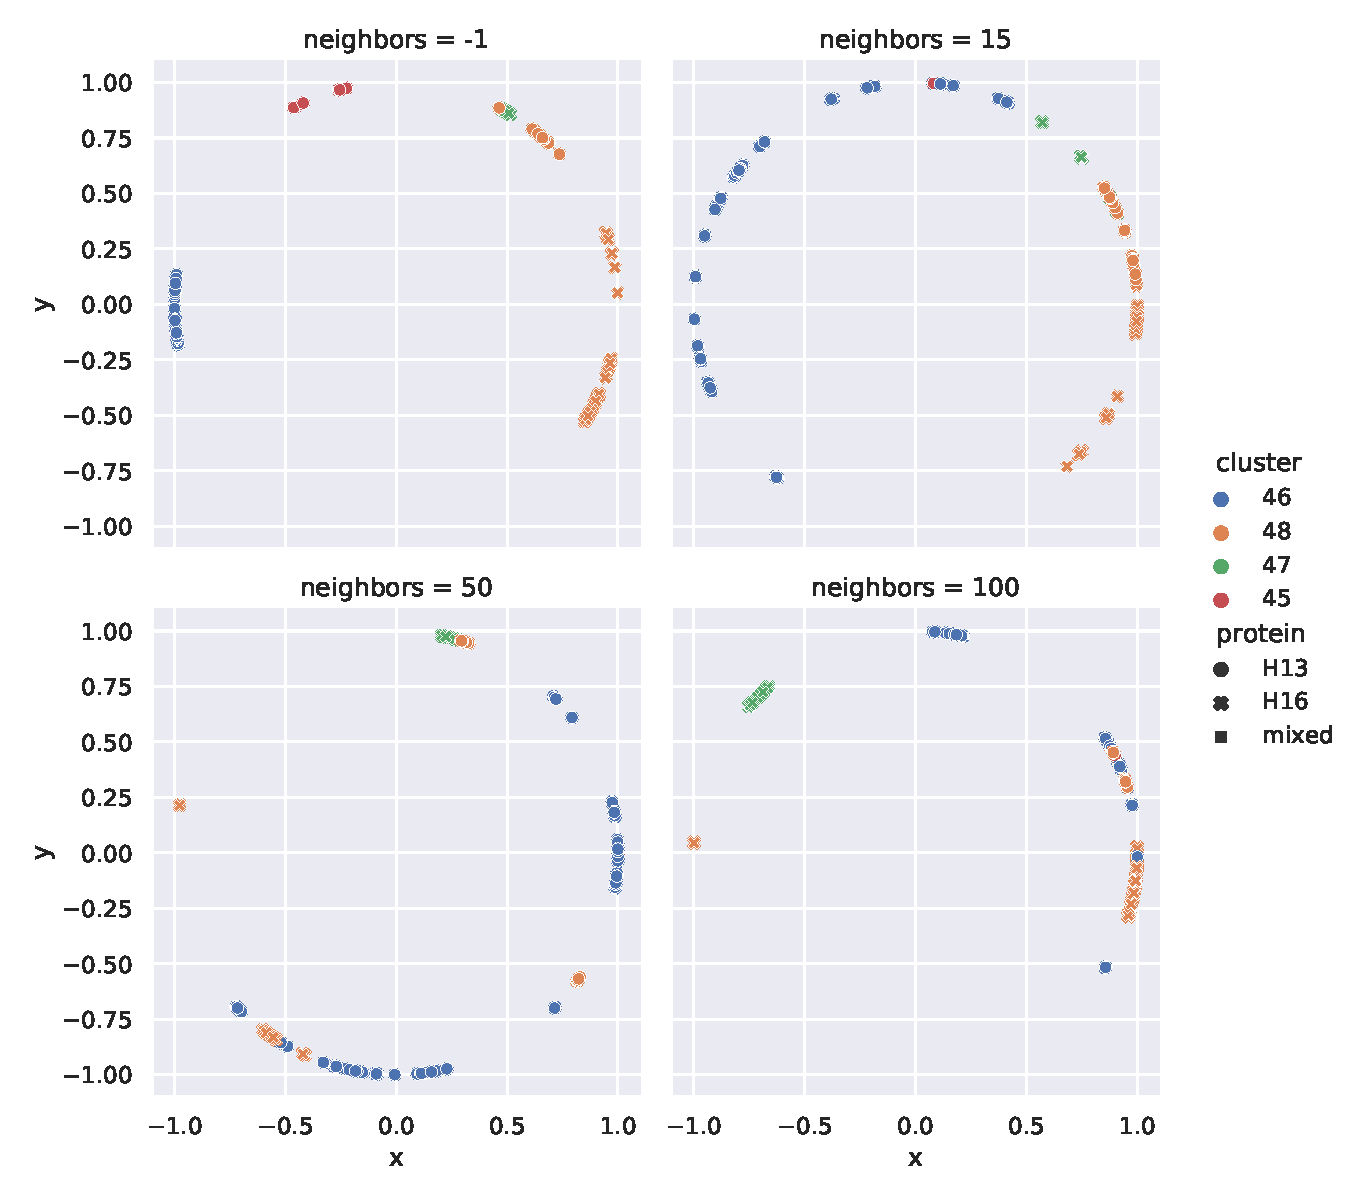
\includegraphics[width=\textwidth]{PCA/Difference_Segment_4_H_metric_cosine.pdf}
    \caption[Comparison of H13/H16 component reductions]{\textbf{Comparison of H13/H16 component reductions.} The subset of sequences from the H13 and H16 clusters in \autoref{fig:PCA_Clusteree_Knee_4} were reduced down to two dimensions enabling simple visualization. Cluster labeling was performed according to \autoref{fig:PCA_Clusteree_Knee_4}. Sole use of \texttt{PCA} (top left picture) as well as the combination with \texttt{UMAP} (other three pictures) was performed as described in \autoref{sec:Dimension_Reduction} with the reduction to two components for visualization. For the combination of \texttt{PCA} and \texttt{UMAP} different values for the neighbors setting were used, the \texttt{UMAP} standard value 15, a average value 50 and the standard value of this project 100. The subtype of the sequences were labeled by different types of points.}
    \label{fig:Reduction_Comparison}
\end{figure}

\vspace{1em}

The visualization of the reduction by \texttt{PCA} is denoted as neighbors value -1 (\autoref{fig:Reduction_Comparison}). It shows five different accumulations of points. Labeling of these points is based on the original clustering example in \autoref{fig:PCA_Cluster_Knee_4}. This is becoming apparent when focusing on the cluster 48 points containing H13 and H16 sequences. That way a fundamental distribution on the points of H13 and H16 can be reviewed as well. 

%When using the right side as possible indication for clustering, all the points and accumulations of points are very close to each other. Nonetheless a separation with a imagined clustering can be made very easy by building two clusters of the blue points, one of the red and green and three of the orange points. Still, all the points related to H13 would be merged with the orange ones of H16 before the orange H16 points would be merged with the green ones of H16. Thereby the difference between H13 and H16, the higher-ranking goal would be not accomplished because the orange points are so close to each other. 
\newpage

The reduction with \texttt{PCA} on the subset results in easy separable accumulations of the cluster 46 and 48 points in \autoref{fig:Reduction_Comparison} (neighbors = -1). The distribution of these points is basically in line with the result shown in \autoref{fig:PCA_Cluster_Knee_4}, as their accumulations are well separated, building the two clusters with the same sequences in both figures. The major difference, however, is the distance between the accumulations of cluster 48 points to each other as well as to the ones of cluster 47. This would probably result in a imaginary clustering of unchanged cluster 46 and 45 and two or three clusters consisting of the cluster 48 points of which one also contains the points of cluster 47. It seems as if the distance of the cluster 47 points and the H13 cluster 48 points is largely affected by the reduction. The difference between cluster 46 and 45 in the \autoref{fig:Reduction_Comparison} (neighbors = -1) picture is on the other hand preserved and would result in clustering similar to \autoref{fig:PCA_Cluster_Knee_4}. In \autoref{fig:PCA_Cluster_Knee_4} cluster 47 and 48 are also relatively close related as they would be linked on the next higher tree-node.

\vspace{1em}

In \autoref{fig:Reduction_Comparison} (neighbors = -1) it appears as if the points of cluster 47 and 48 are possibly quite similar, which is not the case as the \autoref{fig:Precalculated_Cosine} subtrees clearly show the wanted separation of H13 and H16 in cluster 48 as well as the wanted distance to 47. Keeping the lower complexity in mind, the consequence of lowering the dimension by \texttt{PCA} to two dimension seems to preserve most of the information related to the difference of cluster 45 and 46. The difference of the subtype separation inside 48 as well as the overall difference to 47 seems on the other hand to be lost completely and cause the unwanted effects. Since the ground truth separation of \autoref{fig:Precalculated_Cosine} seems to be partially present in \autoref{fig:PCA_Cluster_Knee_4}, by at least separating 47 completely from 48, the higher number of dimensions might be in direct connection to the correct separation of some part of H13 and H16. Therefore, the number of components should be increased to the maximum of 50, that still preserves all functions of \texttt{HDBSCAN} for spanning-tree building. 

\vspace{1em}

Comparing these results to the use of \texttt{UMAP} with different settings of the neighbors value, the impact of this parameter becomes clear. The higher the value, the more crowded the points. This also explains the crowded behavior in \autoref{subfig:Normalisation_UMAP}. Since a neighbors value of 100 was used as standard in this project, the values are overall crowded in groups of at least 100 points. The random subset for \autoref{subfig:Normalisation_UMAP} was reduced by the same setting with \texttt{UMAP} despite the small sample size used there. The small random sample in addition to a high neighbors value resulted in a low number of overall distribution to clarify this behavior. Aside from the example in \autoref{subfig:Normalisation_UMAP} the usage of a high neighbors value through the project was well reasoned and based on the huge size of the dataset used as described in \autoref{sec:Dimension_Reduction}. The same value as well as 15 and 50 neighbors was used on the subset of H13 and H16 segment 4 sequences to visualize the difference. 

\vspace{1em}

None of the settings results in a separation as good as with the sole use of \texttt{PCA}. With the \texttt{UMAP} standard neighbors value of 15 all the points are next to each other and there is no reasonable cluster building possible \autoref{fig:Reduction_Comparison} (neighbors = 15). Furthermore, H13 points would be merged with H16 points before merging with others from H13, thereby breaking the subtype division similar to the \texttt{PCA} use. Aside from the fact that the other points, when using \texttt{PCA}, are well separated. Setting the neighbors value to 50 results in a spreading of the cluster 46 points and mixing with little islands of cluster 48 points \autoref{fig:Reduction_Comparison} (neighbors = 50). With a neighbors value of 100 a separation into imaginary clusters is possible, when ignoring the cluster labeling and only taking the subtypes labeling into consideration. This is, therefore, the only setting with use of \texttt{UMAP} that would provide a more of less reasonable separation of the subtypes in imaginary clusters. However, clusters of different subtypes are closer than to similar subtypes, resulting also in no real subtype separation, even when ignoring the cluster 47 points that might be very sensible to the magnitude of preserved information.

%With normalization and without some information seem to be missing necessary to separate the orange points and the green ones. While on the left side the distance was underestimated to an extend making the orange H13 points and the green H16 points collide, the distance on the right side is overestimated, making the subtype distance of the H13 and H16 orange points to small. Since the separation between red and blue, as well as H13 orange and H16 orange is clearer, the method using normalization is still proved to be the better one, in the circumstances that the location of the green points is caused by the low dimension which is proved by \autoref{fig:PCA_Cluster_Knee_4} showing a separation between 47 and 48 and the right method not producing any better results related to the green points. 
\vspace{1em}

In conclusion, the use of PCA gives the best results compared the ones with \texttt{UMAP}. Still there are challenges to overcome as could be seen with the position of the cluster 47 points. Maybe increasing the information preserved by the \texttt{PCA} would give clearer results as assumed. This project aimed to find high-quality representations of \gls{IAV} genomes for the purpose or clustering in a extend that was never reached before. Therefore, the usability of hybrid \texttt{HDBSCAN} with parameters as good as possible was of higher importance than the use of \texttt{UMAP} at all costs. In the results of the project \texttt{PCA} performed better than \texttt{UMAP} but only with all the tested parameters. Thus, it might be possible to find parameters for \texttt{UMAP} not explored in this project to represent the genomes even better in a equal low-dimension in the future. Also, change of \texttt{UMAP} in favor of \texttt{t-SNE} could be tested in terms of vector representation quality.

\section{The New proposed Classification} \label{sec:Serotype_Classification}

\blindtext

%neue classification vorschlagen blablabla
% vielleicht bisschen evolution black sea gull etc

\begin{figure}[!hbt]
    \centering
    \includegraphics[width=\textwidth, draft]{Results/Clustertree_Segment_4.pdf}
    \caption[Final Segment 4 Clustertree (\Acrshort{PCA})]{\textbf{Final Segment 4 Clustertree (\Acrshort{PCA}).} .}
    %\label{fig:PCA_Clusteree_Final}
\end{figure}

    \glsresetall
    \setcounter{table}{0}
    \setcounter{figure}{0}
    \setcounter{equation}{0}
    
    \chapter{Conclusion} \label{chap:Conclusion}

\blindtext

%precalc ground truth schön und gut aber nicht machbar
%Skalierbarkeit!!!!!
%laufzeit alignment (auch nicht immer perfekt)
%laufzeit kmer und speicher (am besten mit kmer)
%beides braucht TROTZDEM hdbscan (beides keine Cluster tools)
%kmer pca hdb skalierbar ohne exponentiell
%andere viren ohne probleme auch clusterbar (geringe anpassungen)
%new classfiication mit allen segmenten
%tool für jeden nutzbar
%globale classification basierend auf tool mit geringen anforderungen forschung influenza für jeden


    
    %\nocite{*}
    \printbibliography[title=Bibliography]
    
    \listoffigures
    
    \listoftables
    
    \appendix
    
    \appendix
\chapter{Appendix}  \label{chap:A}
    
    \backmatter
    \pagestyle{empty} 
    \renewcommand*{\chapterpagestyle}{empty}
    
    \chapter*{Declaration of Originality}

\end{document}